
\ifdefined\ishandout
  \documentclass[xcolor=x11names, handout]{beamer}
\else
\documentclass[xcolor=x11names]{beamer}
\fi
\ifdefined\isdev
\includeonlyframes{current}
\fi
\usepackage{hyperref}
\hypersetup{
    colorlinks=true,
    linkcolor=blue,
    filecolor=magenta,      
    urlcolor=cyan,
}
\usepackage{mybeamer}
\usepackage{mystyle}
\usepackage[overlay,absolute]{textpos}
\usepackage{bm}
\newcommand{\ubm}[1]{\ubar{\bm{#1}}}
\newcommand{\ubmr}[2]{\ubar{\bm{#1}}^{#2}}
\newcommand{\bmtr}[3]{\bm{#1}^{#3}_{#2}}
\newcommand{\smtr}[3]{{#1}^{#3}_{#2}}

\def\Put(#1,#2)#3{\leavevmode\makebox(0,0){\put(#1,#2){#3}}}
\usepackage{tikz}
\usepackage{pgfplots}
\usetikzlibrary{backgrounds}
\usepackage{adjustbox}
\usepackage{booktabs}       % professional-quality tables
\usepackage{circuitikz}
\setbeamercovered{transparent}
\usetikzlibrary{calc,positioning,shapes}
\usetikzlibrary{patterns,snakes}
\usetikzlibrary{arrows}
\usetikzlibrary{fit}
\newcommand{\midarrow}{\tikz \draw[-triangle 90] (0,0) -- +(.1,0);}
\tikzstyle{every node}=[line width=1pt]
% set arrow type and size by tikz
% alternative to 'Straight Barb' can be 'Latex, Stealth, Computer Modern Rightarrow'.
\usetikzlibrary{arrows.meta}
\tikzset{>={Straight Barb[width=1.0mm,length=1.0mm]}}
\tikzset{block/.style = {draw, fill=white, rectangle,
                  minimum height=3em, minimum width=2cm},
        input/.style = {coordinate},
        output/.style = {coordinate},
        pinstyle/.style = {pin edge={to-,t,black}}
    }

\newcommand{\ubar}[1]{\mkern2mu\underline{\mkern-2mu #1\mkern-2mu}\mkern2mu}
\logo{\copyright Dong Liu\vspace{-0.43cm}\hspace{2cm}}
% \logo{\copyright Dong Liu}

\begin{document}

% define the background opacity
\def\bgopacity{0.3}
% define the background color for stamp block
\def\stampcolor{blue!20}


\begin{frame}
  \title{Perspectives on Probabilistic Graphical Models}
  \subtitle{}
  % 
\includegraphics[height=1cm,width=2cm]{kth_eng_cmyk_wireless.eps}
  \author{ \small Dong Liu
    \\
    \vspace{0.3cm}
    {\it \scriptsize Information Science and Engineering \\
      KTH - Royal Institute of Technology}
    \vspace{0.3cm}
  }
  \vspace{-0.5cm}
  

  \date{
    
\includegraphics[height=2cm,angle=0]{../logo/kth_cmyk_logo.eps}  \\
    % \vspace{0.3cm}
    \scriptsize
    \flushbottom
    \begin{itemize}
    \item ~
    \item Profile page: \href{https://firsthandscientist.github.io/}{https://firsthandscientist.github.io/} \\
    \item Slide is available at: \href{https://github.com/FirstHandScientist/phdthesis}{https://github.com/FirstHandScientist/phdthesis}
    \end{itemize} }
  \titlepage
  
\end{frame}

% decrease the size of font
\scriptsize
%%%%%%%%%%%%%%%%%%%%%%%%%%%%%%%%%%%%%%%%%%%%%%%%%%%%%% 
% ------------------------------------------------
%   Seciton motivation
%%%%%%%%%%%%%%%%%%%%%%%%%%%%%%%%%%%%%%%%%%%%%%%%%%%%%% 


\section{Motivation}

{ \setbeamercolor{background canvas}{bg=hl_bg}
  \setbeamercolor{normal text}{fg=hl_fg}
  \setbeamercolor{frametitle}{fg=hl_fg}
  \begin{frame}
    \usebeamercolor[fg]{normal text}
    \begin{center}
      {\large Why are probabilistic graphical models interesting?}
    \end{center}
  \end{frame}
}
\subsection{Directed}
\begin{frame}{Directed Graph Representation}
  \begin{itemize}
    
    \item 
      \begin{columns}
        \column{0.5\textwidth}
        \hskip 1cm
        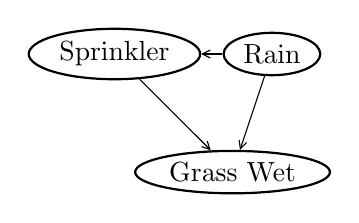
\begin{tikzpicture}
          % \tikzstyle{enode} = [thick, draw=blue, circle, inner sep = 3pt,
          % align=center]
          \tikzstyle{enode} = [thick, draw=black, ellipse, inner sep = 2pt,  align=center]
          \tikzstyle{nnode} = [thick, rectangle, rounded corners = 2pt, minimum size = 0.5cm,draw,inner sep = 2pt]

          \node[enode] (s) at (-0.5, 1.5) {Sprinkler};
          \node[enode] (r) at (1.5, 1.5) {Rain};
          \node[enode] (gw) at (1, 0) {Grass Wet};
          \draw[->] (r) to (s);
          \draw[->] (r) to (gw);
          \draw[->] (s) to (gw);
        \end{tikzpicture}\\
        \centering
        Is the sprinkler working?
        
        \column{0.5\textwidth}
        \hskip -1cm
        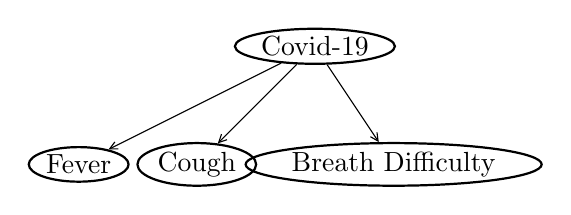
\begin{tikzpicture}
          \tikzstyle{cnode} = [thick, draw=black, ellipse, inner sep = 1pt,  align=center]
          \tikzstyle{nnode} = [thick, rectangle, rounded corners = 0pt,draw,inner sep = 2pt]
          \node[cnode] (virus) at (0, 1.5) {Covid-19};
          \node[cnode] (fever) at (-3, 0) {Fever};
          \node[cnode] (cough) at (-1.5, 0) {Cough};
          \node[cnode] (breath) at (1, 0) {Breath Difficulty};
          \draw[->] (virus) -- (fever);
          \draw[->] (virus) -- (cough);
          \draw[->] (virus) -- (breath);
        \end{tikzpicture}\\
        \centering
        Is the person get contiguous by COVID?
      \end{columns}
    \item 
      \vskip 0.5cm
      \begin{columns}
        \column{0.5\textwidth}
        \hskip 1cm
        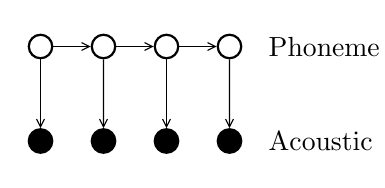
\begin{tikzpicture}[scale=0.8]
          \tikzstyle{enode} = [thick, draw, circle, inner sep = 3pt,  align=center]
          \tikzstyle{cnode} = [thick, fill=black, draw, circle, inner sep = 3pt,  align=center]
          \begin{scope}{scale=0.5, xshift=1cm}
            \node[enode] (x1) at (-2, 0) {};
            \node[enode] (x2) at (-1, 0) {};
            \node[enode] (x3) at (0, 0) {};
            \node[enode] (x4) at (1, 0) {};
            \node[text width=1cm, right = 0.2cm of x4] {Phoneme};
            \node[cnode] (y1) at (-2, -1.5) {};
            \node[cnode] (y2) at (-1, -1.5) {};
            \node[cnode] (y3) at (0, -1.5) {};
            \node[cnode] (y4) at (1, -1.5) {};
            \node[text width=1cm, right = 0.2cm of y4] {Acoustic};

            \draw[->] (x1) to (x2);
            \draw[->] (x2) to (x3);
            \draw[->] (x3) to (x4);

            \draw[->] (x1) to (y1);
            \draw[->] (x2) to (y2);
            \draw[->] (x3) to (y3);
            \draw[->] (x4) to (y4);

          \end{scope}
        \end{tikzpicture}
        \vskip 0.1cm
        \centering
        Speech Recognition
        \column{0.5\textwidth}
        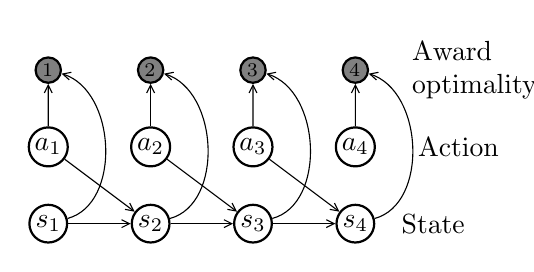
\begin{tikzpicture}[scale=0.65]
          \tikzstyle{enode} = [thick, draw, circle, inner sep = 1pt,  align=center]
          \tikzstyle{cnode} = [thick, fill=gray, draw, circle, inner sep = 1pt,  align=center]
          \begin{scope}{scale=0.5, xshift=1cm}
            \node[cnode] (o1) at (-2, 1.5) {$\Oo_1$};
            \node[cnode] (o2) at (0, 1.5) {$\Oo_2$};
            \node[cnode] (o3) at (2, 1.5) {$\Oo_3$};
            \node[cnode] (o4) at (4, 1.5) {$\Oo_4$};
            \node[text width=1cm, right = 0.2cm of o4] {\begin{tabular}{l}Award\\optimality\end{tabular}};

            \node[enode] (a1) at (-2, 0) {$a_1$};
            \node[enode] (a2) at (0, 0) {$a_2$};
            \node[enode] (a3) at (2, 0) {$a_3$};
            \node[enode] (a4) at (4, 0) {$a_4$};
            \node[text width=1cm, right = 0.4cm of a4] {Action};
            \node[enode] (s1) at (-2, -1.5) {$s_1$};
            \node[enode] (s2) at (0, -1.5) {$s_2$};
            \node[enode] (s3) at (2, -1.5) {$s_3$};
            \node[enode] (s4) at (4, -1.5) {$s_4$};
            \node[text width=1cm, right = 0.2cm of s4] {State};

            \draw[->] (s1) to (s2);
            \draw[->] (s2) to (s3);
            \draw[->] (s3) to (s4);
            \draw[->] (a1) to (s2);
            \draw[->] (a2) to (s3);
            \draw[->] (a3) to (s4);
            \draw[->] (s1) to [out=15, in=-15] (o1);
            \draw[->] (s2) to [out=15, in=-15] (o2);
            \draw[->] (s3) to [out=15, in=-15] (o3);
            \draw[->] (s4) to [out=15, in=-15] (o4);
            \foreach \x in {1,...,4}{
              \draw[->] (a\x) to (o\x);
            }

          \end{scope}
          
        \end{tikzpicture}
        \centering
        Decision-making (reinforcement learning)
      \end{columns}
    
  \end{itemize}

\end{frame}


\subsection{Undirected}
\begin{frame}{Undirected Graph Representations}
  \begin{itemize}
  \item % image segmentation
        \begin{tikzpicture}
          \tikzstyle{enode} = [thick, draw, thick,fill=white, circle, inner sep = 2pt,  align=center]
          \tikzstyle{cnode} = [thick, fill=gray, draw, circle, inner sep = 2pt,  align=center]
          \begin{scope}{scale=0.4}
            \node[inner sep=0pt] (img) at (-8,0) {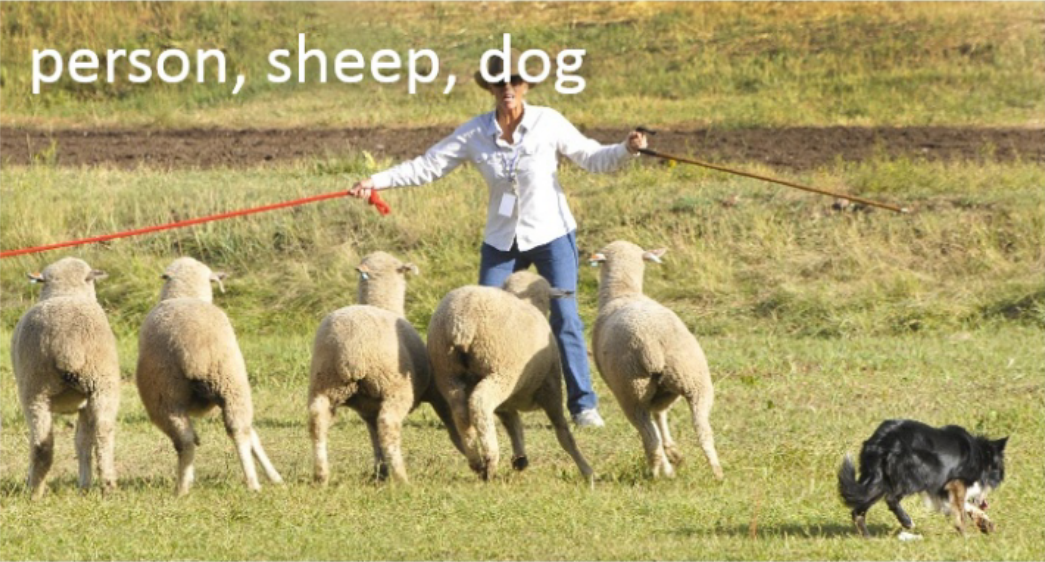
\includegraphics[width=.25\textwidth]{images/illustrate/cocoDemo.png}};
            \node[black, above=0.05 of img] () {\tiny Coco};
          \end{scope}
          \begin{scope}{scale=0.4}
            \node[inner sep=0pt] (slam) at (0,0) {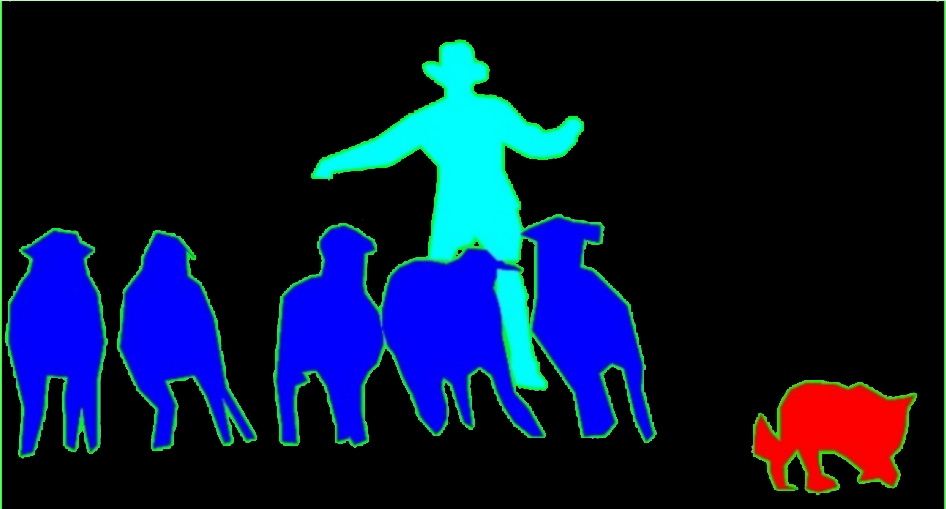
\includegraphics[width=.25\textwidth]{images/illustrate/cocoSlam.png}};
            
          \end{scope}
          
          \begin{scope}[local bounding box=crf, scale=0.6, shift={(-8, -1)}]
            \draw (0,0) grid (4,3);
            \foreach \i in {0,...,4}{
              \foreach \j in {0,...,3} {
                \node[enode] (x\i\j) at (\i, \j) {};
                \node[cnode] (y\i\j) at ($(\i, \j) + (-0.5, -0.5)$) {};
                \draw[-] (x\i\j) to (y\i\j);
              }
            }
            \node[right = 0.02 of x43] {\tiny Label};
            \node[left = 0.02 of y00] {\tiny Pixel};
          \end{scope}
          
        \end{tikzpicture}
        \vskip 0.1cm
        \centering
        Vision Perception
        \item % digital communication
        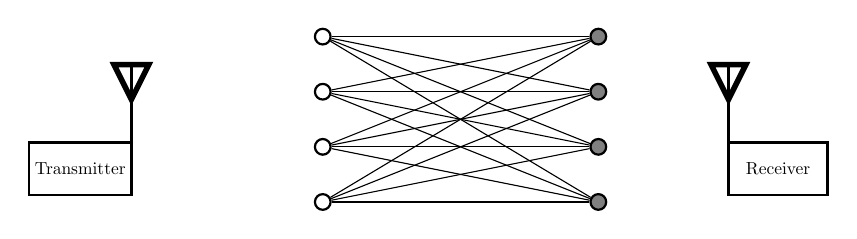
\begin{tikzpicture}[scale=0.7]
          \tikzstyle{enode} = [thick, draw, circle, inner sep = 2pt,  align=center]
          \tikzstyle{cnode} = [thick, fill=gray, draw, circle, inner sep = 2pt,  align=center]
      
          \begin{scope}[local bounding box=mrf]{scale=0.15, shift={(-2,10)}}
            \foreach \i in {-3,...,0} {
              \node[cnode] (x\i) at (0, \i) {};
              \node[enode] (y\i) at (-5, \i) {};
            }
            \foreach \i in {-3,...,0} {
              \foreach \j in {-3,...,0} {
                \draw (x\i) to (y\j) ;
              }
            }

          \end{scope}

          \begin{scope}[shift={($(mrf)+(-1.5,0)$)}, scale=0.9, every node/.append style={transform shape}]
          \node[block](tx) at (-6,-1) {Transmitter};
          \node[antenna] at (tx.east) {};
          \node[block,right = 12 of tx](rx){Receiver};
          \node[antenna,xscale=-1] at (rx.west) {};
          \end{scope}
        \end{tikzpicture}\\
        \centering
        Digital communication
      \item % Solid physics
        \begin{columns}
          \column{0.5\textwidth}
          \centering
        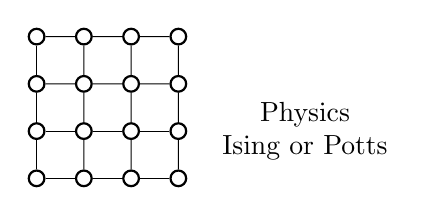
\begin{tikzpicture}
          \tikzstyle{enode} = [thick, draw, circle, inner sep = 2pt,  align=center]
          \tikzstyle{cnode} = [thick, fill=gray, draw, circle, inner sep = 3pt,  align=center]
      
          \begin{scope}[local bounding box=mrf, scale=0.6]
            \node[enode] (x11) at (0, 0) {};
            \node[enode] (x12) at (1, 0) {};
            \node[enode] (x13) at (2, 0) {};
            \node[enode] (x14) at (3, 0) {};
            \node[enode] (x21) at (0, 1) {};
            \node[enode] (x22) at (1, 1) {};
            \node[enode] (x23) at (2, 1) {};
            \node[enode] (x24) at (3, 1) {};
            \node[enode] (x31) at (0, 2) {};
            \node[enode] (x32) at (1, 2) {};
            \node[enode] (x33) at (2, 2) {};
            \node[enode] (x34) at (3, 2) {};
            \node[enode] (x41) at (0, 3) {};
            \node[enode] (x42) at (1, 3) {};
            \node[enode] (x43) at (2, 3) {};
            \node[enode] (x44) at (3, 3) {};
            \node[black] (text) [right=0.1 of x24] {\begin{tabular}{c}Physics \\Ising or Potts \end{tabular}};
            \draw (x11)--(x12)--(x13)--(x14);
            \draw (x21)--(x22)--(x23)--(x24);
            \draw (x31)--(x32)--(x33)--(x34);
            \draw (x41)--(x42)--(x43)--(x44);

            \draw (x11)--(x21)--(x31)--(x41);
            \draw (x12)--(x22)--(x32)--(x42);
            \draw (x13)--(x23)--(x33)--(x43);
            \draw (x14)--(x24)--(x34)--(x44);
          \end{scope}
        \end{tikzpicture}\\
        \centering
        
        \column{0.5\textwidth}
        \begin{itemize}[label=$\bullet$]
        \item Error-control codes
        \item Computational biology
        \item Natural language processing
        \item etc.
        \end{itemize}
      \end{columns}
  \end{itemize}


\end{frame}


%%% Local Variables:
%%% mode: latex
%%% TeX-master: "../ppgm_slide"
%%% End:

%%%%%%%%%%%%%%%%%%%%%%%%%%%%%%%%%%%%%%%%%%%%%%%%%%%%%% 
% ------------------------------------------------

%%%%%%%%%%%%%%%%%%%%%%%%%%%%%%%%%%%%%%%%%%%%%%%%%%%%%% 
% \section{Content}
% \subsection{Content}
% \begin{frame}{\large Content}
%   \begin{itemize}[label=$\bullet$]
%   \item Background: Probabilistic graphical models (PGM)
%   \item Common usage of PGMs
%   \item High-level view of inference
%   \item Play inference with neural networks
%   \item Summary
%   \end{itemize}
  
% \end{frame}



% \begin{frame}{\large Content}
%   \begin{tikzpicture}
%     \tikzstyle{enode} = [thick, draw=black, ellipse, inner sep = 2pt,  align=center]
%     \node[enode] (fd) at (0,0) {Fundamental Problems};
%     \node[enode] (fd) at (0,-1) {General Methods};
%     \node[enode] (fd) at (0,-2) {Gibbs Simpling};
%     \node[enode] (fd) at (0,-3) {Mean Field};
%     \node[enode] (fd) at (0,-4) {Loopy Belief Propagation};
%     \node[enode] (fd) at (0,-5) {Generalized Belief Propagation};
%     \node[enode] (fd) at (0,-6) {Our approximation: RENN};
%     \node[enode] (fd) at (0,-7) {Application scenarios/examples};
%     \node[enode] (fd) at (0,-8) {Some numerical results};
%   \end{tikzpicture}

% \end{frame}

%%%%%%%%%%%%%%%%%%%%%%%%%%%%%%%%%%%%%%%%%%%%%%%%%%%%%% 
% ------------------------------------------------
% section core
%%%%%%%%%%%%%%%%%%%%%%%%%%%%%%%%%%%%%%%%%%%%%%%%%%%%%% 

\section{Preliminary}
\subsection{Basics}
{ \setbeamercolor{background canvas}{bg=hl_bg}
  \setbeamercolor{normal text}{fg=hl_fg}
  \setbeamercolor{frametitle}{fg=hl_fg}
  \begin{frame}{A Guide to This Dissertation}
    \usebeamercolor[fg]{normal text}
    \centering
    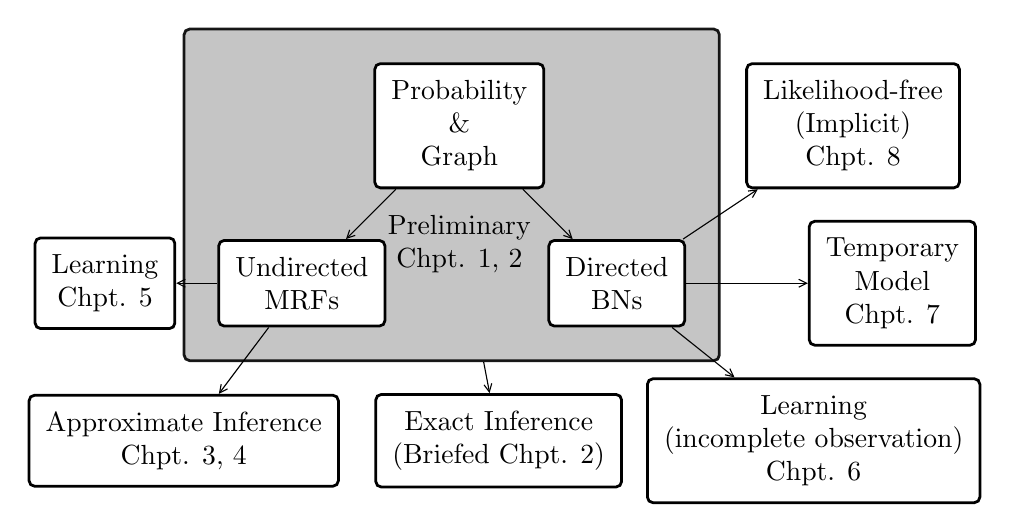
\begin{tikzpicture}
      \tikzstyle{nnode} = [rectangle, rounded corners=2pt, inner sep = 6pt,  align=center]
      \tikzstyle{rnode} = [draw=black, rectangle, rounded corners=2pt, inner sep = 6pt, align=center]

      \begin{scope}[xshift=-0.5cm]
        \node[rnode, fill=white, text=black] (PandG) at (0,0) {Probability\\ \& \\ Graph};
        \node[rnode, fill=white, text=black] (mrf) at (-2,-2) {Undirected\\
          MRFs};
        \node[rnode, fill=white, text=black] (bn) at (2,-2) {Directed\\
          BNs};
        \begin{scope}[on background layer]
          \node[rnode, inner sep = 12pt, fill=gray!50, opacity=0.9, fit=(PandG)(mrf)(bn)] (core) {};
          \node[nnode] at (0,-1.5) {Preliminary \\ Chpt. 1, 2};
        \end{scope}
      \end{scope}
      \draw[black,->] (PandG) to (mrf);
      \draw[black,->] (PandG) to (bn);
      
      \node[rnode, fill=white, text=black] (exact) at (0, -4) {Exact Inference \\ (Briefed Chpt. 2)};
      \draw[black,->] (core) to (exact);
      
      \node[rnode, fill=white, text=black] (apprx) at (-4, -4) {Approximate Inference\\
        Chpt. 3, 4};
      \node[rnode, fill=white, text=black] (mrfLearn) at (-5, -2) {Learning\\ Chpt. 5};
      
      \draw[black,->] (mrf) to (apprx);
      \draw[black,->] (mrf) to (mrfLearn);

      \node[rnode, fill=white, text=black] (em) at (4, -4) {Learning \\ (incomplete observation) \\ Chpt. 6};
      \node[rnode, fill=white, text=black] (hmm) at (5, -2) {Temporary\\Model \\ Chpt. 7};
      \node[rnode, fill=white, text=black] (llkFree) at (4.5, 0) {Likelihood-free\\
        (Implicit) \\ Chpt. 8};
      
      \draw[black,->] (bn) to (em);
      \draw[black,->] (bn) to (hmm);
      \draw[black,->] (bn) to (llkFree);
      

      

    \end{tikzpicture}
  \end{frame}
}

\begin{frame}{What are Probabilistic Graphical Models}
  \onslide<1->{
    Informally...
    \begin{itemize}[label={$\bullet$}]
    \item attributes of our interests in a system $\rightarrow$ variable nodes
    \item relationship of these factors $\rightarrow$ structures of a graph
    \end{itemize}
    Intrinsic property: \textbf{reasoning with uncertainty}
  }\\
  \vskip 0.8cm
  
    A directed/undirected graph encoding dependencies/indepedencies of distribution $p(\bm{x}; \bm{\theta})$:
    \begin{itemize}[label={$\bullet$}]
    \item A BN/Generative model is a directed graph
      \begin{itemize}[label={$\bullet$}]
      \item $p(\bm{x}; \bm{\theta}) = \prod_{n=1}^{N}p(x_n| \Pp(x_n))$
      \item $\Pp(\cdot)$ are parent nodes
      \item the local functions are proper distributions
      \end{itemize}
      
    \item An MRF denoted by an undirected graph $\Gg(\Vv, \Ee)$
      \begin{itemize}[label=$\bullet$]
      \item The probability distribution (Gibbs distribution) is $p(\bm{x}; \bm{\theta}) = \frac{1}{Z(\bm{\theta})} \prod_{a\in\Ii} \psi_a(\bm{x}_a; \bm{\theta}_a)$
      \item  $a$ indexes potential functions $\Ii=\{\psi_A, \psi_B, \cdots, \psi_M\}$
      \item $Z(\bm{\theta}) = \sum_{\bm{x}}\prod_{a} \psi_a(\bm{x}_a;\bm{\theta}_a)$.
      \end{itemize}
    \end{itemize}
  
  
\end{frame}
\begin{frame}{Usage of Graphical Models}
  \begin{itemize}[label={$\bullet$}]
  \item The common inference problems:
    \begin{itemize}[label={$\bullet$}]
    \item Computing the likelihood of observed data.
    \item Computing the marginals distribution $p(\bm{x}_A)$ over particular subset $A \subset \Vv$ of nodes
    \item Computing the conditional distribution $p(\bm{x}_A | \bm{x}_{B})$, 
    \item Computing the partition function or the Helmholtz free energy (for MRFs)
    \end{itemize}
  \item Learning:
    \begin{itemize}[label=$\bullet$]
      \item To model or determine $p(\bm{x}; \bm{\theta})$.
      \end{itemize}
  \end{itemize}
  

  
    Two key components interacting with each other:
    \begin{figure}[!t]
      \centering
      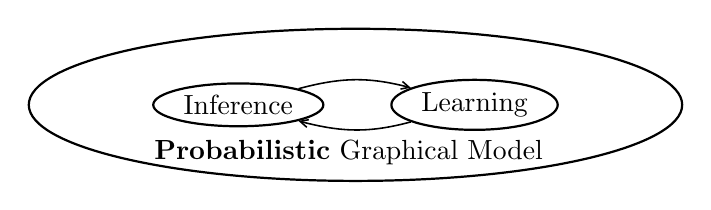
\begin{tikzpicture}
        \tikzstyle{cnode} = [thick, draw=black, ellipse, inner sep = 2pt,  align=center]
        \tikzstyle{fnode} = [thick, draw=black, ellipse, inner sep = 10pt,  align=center]
        
        \node[cnode] (infn) at (0,0) {Inference};
        \node[cnode] (lern) at (3,0) {Learning};
        
        \node[fnode, fit=(infn)(lern)] (box) {};
        \node[] at (1.4, -0.6) {\textbf{Probabilistic} Graphical Model};
        \draw[->,line width=0.2mm] (infn) to[out=15, in=165] (lern);
        \draw[->,line width=0.2mm] (lern) to[out=195, in=-15] (infn);
      \end{tikzpicture}

    \end{figure}
  

\end{frame}








%%%%%%%%%%%%%%%%%%%%%%%%%%%%%%%%%%%%%%%%%%%%%%%%%%%%%% 
% ------------------------------------------------
%%%%%%%%%%%%%%%%%%%%%%%%%%%%%%%%%%%%%%%%%%%%%%%%%%%%%% 
% \section{Inference}



\subsection{Intuition of Message Passing}
\begin{frame}{What is the state of $x$?}
  \framesubtitle{A toy example}
  Assume that we are interested into the state of node $i$ in an MRF, it can be answered by
  \begin{itemize}[label={$\bullet$}]
  \item the probability $p(x_i)$, or
  \item an empirical version, a collection of samples $\left\{ x_i^n \right\}_{n=1}^{N}$
  \end{itemize}
  It is similar for the case when $\bm{x}$ is of interests, instead of $x_i$.
  \begin{figure}
    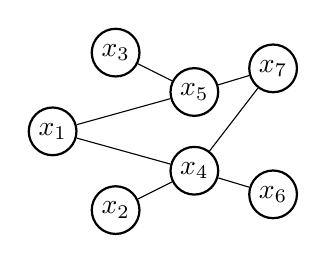
\begin{tikzpicture}
      % \tikzstyle{enode} = [thick, draw=blue, circle, inner sep = 3pt,
      % align=center]
      \tikzstyle{enode} = [thick, draw=black, circle, inner sep = 2pt,  align=center]
      \node[enode] (x1) at (-0.8,0) {$x_1$};
      \node[enode] (x2) at (0,-1) {$x_2$};
      \node[enode] (x3) at (0,1) {$x_3$};
      \node[enode] (x4) at (1,-0.5) {$x_4$};
      \node[enode] (x5) at (1,0.5) {$x_5$};
      \node[enode] (x6) at (2,-0.8) {$x_6$};
      \node[enode] (x7) at (2,+0.8) {$x_7$};

      \draw[-] (x1) to (x4);
      \draw[-] (x1) to (x5);
      \draw[-] (x2) to (x4);
      
      \draw[-] (x3) to (x5);
      \draw[-] (x4) to (x6);
      \draw[-] (x4) to (x7);
      \draw[-] (x5) to (x7);
    \end{tikzpicture}
    \captionsetup{labelformat=empty,justification=centering}
    \caption{what is the state of $x_4$}
    
  \end{figure}
  
\end{frame}

\begin{frame}{What is the state of $x$?}
  \begin{columns}
    \column{0.5\textwidth}
    {Gibbs sampling: let us guess by sampling}
    \vskip 0.5cm
   Sample iteratively: $  x_i \sim p(x_i|\bm{x}_{-i}) \sim p(x_i,\bm{x}_{-i})$
  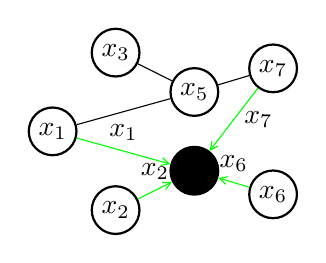
\begin{tikzpicture}
        % \tikzstyle{enode} = [thick, draw=blue, circle, inner sep = 3pt,
        % align=center]
        \tikzstyle{enode} = [thick, draw=black, circle, inner sep = 2pt,  align=center]
        \node[enode] (x1) at (-0.8,0) {$x_1$};
        \node[enode] (x2) at (0,-1) {$x_2$};
        \node[enode] (x3) at (0,1) {$x_3$};
        \node[enode, fill=\stampcolor] (x4) at (1,-0.5) {$x_4$};
        \node[enode] (x5) at (1,0.5) {$x_5$};
        \node[enode] (x6) at (2,-0.8) {$x_6$};
        \node[enode] (x7) at (2,+0.8) {$x_7$};

        \draw[green,->] (x1) to node[black,above] {$x_1$} (x4);
        \draw[-] (x1) to (x5);
        \draw[green,->] (x2) to node[black,above] {$x_2$} (x4);
        
        \draw[-] (x3) to (x5);
        \draw[green,->] (x6) to node[black,above] {$x_6$} (x4);
        \draw[green,->] (x7) to node[black,right] {$x_7$} (x4);
        \draw[-] (x5) to (x7);
      \end{tikzpicture}
      \vskip 0.5cm
      Queries by collected samples $\left\{ \bm{x}^n \right\}_{1}^{N}$.
      
    \column{0.5\textwidth}
    Mean Field and BP: \textit{message in form of sample values $\rightarrow$ message in form of belief}
    \vskip 0.5cm
    Propagating beliefs iteratively
      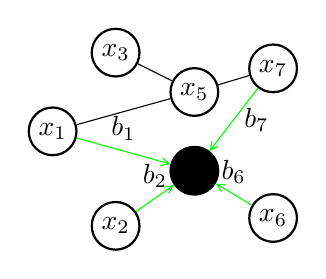
\begin{tikzpicture}
      \tikzstyle{enode} = [thick, draw=black, circle, inner sep = 2pt,  align=center]
      \node[enode] (x1) at (-0.8,0) {$x_1$};
      \node[enode] (x2) at (0,-1.2) {$x_2$};
      \node[enode] (x3) at (0,1) {$x_3$};
      \node[enode, fill=\stampcolor] (x4) at (1,-0.5) {$x_4$};
      \node[enode] (x5) at (1,0.5) {$x_5$};
      \node[enode] (x6) at (2,-1.1) {$x_6$};
      \node[enode] (x7) at (2,+0.8) {$x_7$};

      \draw[green,->] (x1) to node[black,above=0.05mm] {$b_1$} (x4);
      \draw[-] (x1) to (x5);
      \draw[green,->] (x2) to node[black,above=0.05mm] {$b_2$}(x4);
      
      \draw[-] (x3) to (x5);
      \draw[green,->] (x6) to node[black,above=0.05mm] {$b_6$} (x4);
      \draw[green,->] (x7) to node[black,right] {$b_7$} (x4);
      \draw[-] (x5) to (x7);
    \end{tikzpicture}
    \vskip 0.5cm
    Queries by collected samples $\left\{ b_i\right\}$.

    % Corresponding to minimization of \textbf{variational free energy $F_v(b)$  with trial $b$ in fully-factorized form for univariant $\{b_i\}$}.
    \end{columns}
    \let\thefootnote\relax\footnotetext{
      Intuition from \textit{Gibbs (variational) free energy}
        \begin{equation*}
          F_V(b) = \mathrm{KL}(b( \bm{x}) || p(\bm{x}; \bm{\theta})) - \log{Z(\bm{\theta})}
        \end{equation*}
        with trial $b(\bm{x})$. Instance: Bethe free energy.
        }
\end{frame}

% \begin{frame}{What is the state of $x$?}
%   Naive Mean Field: \textbf{message in form of sample values $\rightarrow$ message in form of belief}
%   \begin{figure}
    
%     \begin{tikzpicture}
%       \tikzstyle{enode} = [thick, draw=black, circle, inner sep = 2pt,  align=center]
%       \node[enode] (x1) at (-0.8,0) {$x_1$};
%       \node[enode] (x2) at (0,-1.2) {$x_2$};
%       \node[enode] (x3) at (0,1) {$x_3$};
%       \node[enode, fill=gray] (x4) at (1,-0.5) {$x_4$=?};
%       \node[enode] (x5) at (1,0.5) {$x_5$};
%       \node[enode] (x6) at (2,-1.1) {$x_6$};
%       \node[enode] (x7) at (2,+0.8) {$x_7$};

%       \draw[->] (x1) to node[above=0.05mm] {$b_1$} (x4);
%       \draw[-] (x1) to (x5);
%       \draw[->] (x2) to node[above=0.05mm] {$b_2$}(x4);
      
%       \draw[-] (x3) to (x5);
%       \draw[->] (x6) to node[above=0.05mm] {$b_6$} (x4);
%       \draw[->] (x7) to node[right] {$b_7$} (x4);
%       \draw[-] (x5) to (x7);
%     \end{tikzpicture}
%   \end{figure}
%   Corresponding to minimization of \textbf{variational free energy $F_v(b)$  with trial $b$ in fully-factorized form for univariant $\{b_i\}$}.
%   \let\thefootnote\relax\footnotetext{\tiny
%     Iterative sampling $\rightarrow$ iterative belief update via  
%     \begin{equation*}
%       \log{b_i(x_i)} \propto \sum_{a \in \mathrm{ne}_i} \sum_{\bm{x}_{a} \backslash x_i} \prod_{j\in {a}\backslash i} b_j(x_j)\log{\phi_{a}}(\bm{x}_{a};\bm{\theta}_{a}).
%     \end{equation*}  
%   }
% \end{frame}

% \begin{frame}{What is the state of $x$?}
%   \framesubtitle{Belief propagation (BP): let us guess by propagating belief}
%   \onslide<1->{

%     Proposed by Pearl (1982) for Bayesian networks (tree-structured graphs), which then widely used for general graphs (loopy BP).
    
%     {Yedidia, et al, connected the loopy BP with stationary points of \textbf{Bethe free energy}
%       \begin{align*}
%         F_{Bethe}(b) = \sum_{a\in \Ff} \sum_{\bm{x}_{a}}
%         b_{a}(\bm{x}_{a})\log{\frac{b_{a}(\bm{x}_{a})}{\phi_{a}(\bm{x}_{a})}
%         } -  \sum_{i=1}^{N} (|\mathrm{ne}_i| - 1) \sum_{x_i} b_i(x_i) \log{b_i(x_i)},
%       \end{align*}
%     }
    
%     Corresponding to minimization of approximated \textbf{variational free energy $F_v(b)$  with trial $b$ includes $\{b_i\}$ and $\{b_a\}$}.

%   }
%   \let\thefootnote\relax\footnotetext{\tiny
%     \vskip -0.8cm
%     \begin{align*}
%       \mathrm{msg: factor~ to~ variable} ~~ m_{a\rightarrow i}(x_i) & \propto \sum_{\bm{x}_{a} \backslash x_i}
%                                                                       \phi_{a}(\bm{x}_{a}) \prod_{j \in a \backslash i} m_{j\rightarrow a}(x_j), \\
%       \mathrm{msg: variable~ to~ factor} ~~  m_{j\rightarrow a}(x_j) & \propto  \prod_{a^{\prime} \in \mathrm{ne}_j
%                                                                        \backslash a} m_{a^{\prime}\rightarrow j}(x_j)
%     \end{align*}
%     See, D. Liu, M. T. Vu, Z. Li, and Lars K. Rasmussen. $\alpha$ belief propagation for approximate inference. 2020 \\
%     D. Liu, N. N. Moghadam, L. K. Rasmussen, etc. $\alpha$ belief propagation as fully factorized approximation. In
%     GlobalSIP, 2019.
%     for alternative view to loopy BP.
%   }
  
% \end{frame}



% { \setbeamercolor{background canvas}{bg=hl_bg}
%   \setbeamercolor{normal text}{fg=hl_fg}
%   \setbeamercolor{frametitle}{fg=hl_fg}
%   \begin{frame}
%     \usebeamercolor[fg]{normal text}
%     \begin{center}
%       {\large
%         Play with
%         \textbf{Gibbs (variational) free energy}
%         \begin{equation*}
%           F_V(b) = \mathrm{KL}(b( \bm{x}) || p(\bm{x}; \bm{\theta})) - \log{Z(\bm{\theta})}
%         \end{equation*}
%         with trial $b(\bm{x})$.
%       }
%     \end{center}
    
%   \end{frame}
% }


%%% Local Variables:
%%% mode: latex
%%% TeX-master: "../ppgm_slide"
%%% End:


%%%%%%%%%%%%%%%%%%%%%%%%%%%%%%%%%%%%%%%%%%%%%%%%%%%%%% 
% ------------------------------------------------
% section inference
%%%%%%%%%%%%%%%%%%%%%%%%%%%%%%%%%%%%%%%%%%%%%%%%%%%%%% 

\section{Inference}
\subsection{Alpha-BP}
{ \setbeamercolor{background canvas}{bg=hl_bg}
  \setbeamercolor{normal text}{fg=hl_fg}
  \setbeamercolor{frametitle}{fg=hl_fg}
  \begin{frame}
    \usebeamercolor[fg]{normal text}
    \begin{center}
      {
        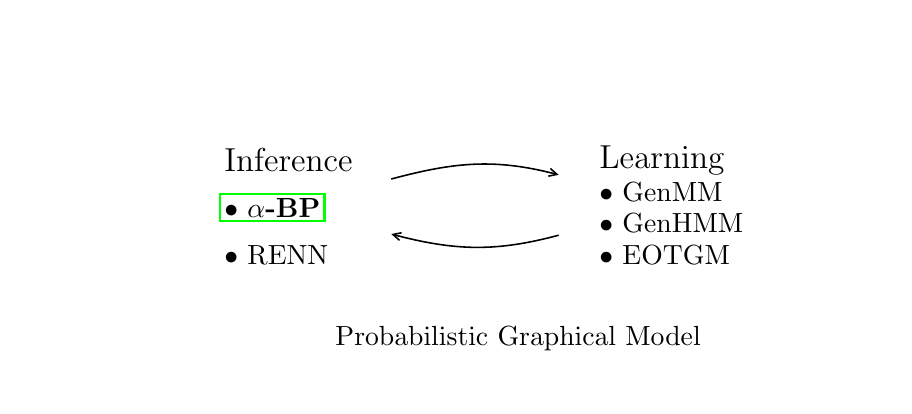
\begin{tikzpicture}
          \tikzstyle{cnode} = [thick, draw=white, ellipse, inner sep = 2pt,  align=center]
          \tikzstyle{fnode} = [thick, draw=white, ellipse, inner sep = 10pt,  align=center]
          \tikzstyle{rnode} = [thick, rectangle, inner sep = 1.5pt,  align=left]
          \node[rnode] (inf) at (-2, 0) {\large Inference};
          \node[rnode, below = 0.6cm of inf.west, anchor=west, draw=green] (abp) {$\bullet$ \textbf{$\alpha$-BP}};
          \node[rnode, below = 1.2cm of inf.west, anchor=west] (renn) {$\bullet$ RENN};
          \node[cnode, fit=(abp)(inf)(renn)] (infn) {};
          
          \node[rnode, right = 3 of inf] (lern) {\large Learning};
          \node[rnode, below = 0.4 of lern.west, anchor=west] (genmm) {$\bullet$ GenMM};
          \node[rnode, below = 0.8 of lern.west, anchor=west] (genhmm) {{$\bullet$} GenHMM};
          \node[rnode, below = 1.2 of lern.west, anchor=west] (lfree) {{$\bullet$} EOTGM};
          \node[cnode, fit=(lern)(genmm)(genhmm)(lfree)] (learn) {};

          \node[fnode, fit=(infn)(lern)] (box) {};

          
          \node[below right = 0.5 and -0.5 of infn] {{Probabilistic} Graphical Model};
          \draw[->,line width=0.2mm] (infn) to[out=15, in=165] (learn);
          \draw[->,line width=0.2mm] (learn) to[out=195, in=-15] (infn);
        \end{tikzpicture}
      }
    \end{center}
    
  \end{frame}
}

\begin{frame}{Alternative Veiw of BP: $\alpha$-BP}
  Input:
  \begin{columns}
    \column{0.6\textwidth}
    \begin{itemize}[label=$\bullet$]
    \item A pairwise Markov random field: $p(\bm{x}) \propto \prod_{{s\in \Vv}} \phi_s(x_s) \prod_{(s,t) \in \Ee} \phi_{st}(x_s, x_t)$
    \item A trial distribution: $q(\bm{x}) \propto \prod_{{s\in \Vv}} \tilde{\phi}_s(x_s) \prod_{(s,t) \in \Ee} \tilde{\phi}_{st}(x_s, x_t)$ with factorization $\tilde{\phi}_{s,t}(x_s, x_t) := m_{st}(x_t) m_{ts}(x_s)$
    \item A metric: $\alpha$-Divergence 
    \end{itemize}
    
    \column{0.4\textwidth}
    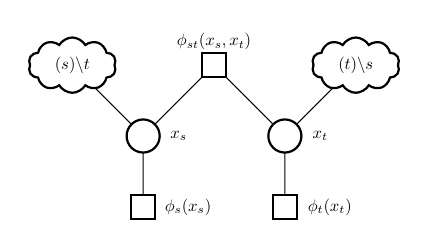
\begin{tikzpicture}
      \begin{scope}[scale=0.6, every node/.append style={transform shape}]
        \tikzstyle{enode} = [thick, draw=black, circle, inner sep = 4pt, minimum size = 0.7cm, align=center]
        \tikzstyle{nnode} = [thick, rectangle, rounded corners = 0pt, minimum size = 0.5cm,draw,inner sep = 2pt]
        \tikzstyle{cnode} = [thick, cloud, draw,cloud puffs=10, cloud puff arc=120, aspect=2, inner ysep=4pt]
        \node[cnode] (pajk) at (3, 1.5) {$\Nn(t)\backslash s$};
        \node[cnode] (paik) at (-3, 1.5) {$\Nn(s)\backslash t$};
        \node[nnode] (tk) at (0, 1.5) {};
        \node[] at ($(tk) + (0, 0.5)$) {$\phi_{st}(x_s, x_t)$};
        \node[enode] (xi) at (-1.5 ,0) {};
        \node[] at ($(xi) + (0.75,0)$) {$x_s$};
        \node[nnode] (fi) at (-1.5 , -1.5) {};
        \node[] at ($(fi) + (0.95,0)$) {$\phi_s(x_s)$};
        \node[enode] (xj) at (1.5 ,0) {};
        \node[] at ($(xj) + (0.75,0)$) {$x_t$};
        \node[nnode] (fj) at (1.5 , -1.5) {};
        \node[] at ($(fj) + (0.95,0)$) {$\phi_t(x_t)$};
        % connections
        \draw[-] (xi) to (fi);
        \draw[-] (xi) to (tk);
        \draw[-] (xi) to (paik);
        \draw[-] (xj) to (fj);
        \draw[-] (xj) to (tk);
        \draw[-] (xj) to (pajk);
      \end{scope}
    \end{tikzpicture}
    \centering{$\Gg:=(\Vv, \Ee)$}
  \end{columns}
  \vskip 1cm
  Approximate local minimization:
  \begin{itemize}[label=$\bullet$]
  \item Direct minimization: $ \!\!\!\uargmin{\tilde{\phi}_{ts}^{\mathrm{new}}(x_t, x_s)}\!\!\!\! \Dd_{\alpha_{ts}}\!\!\left(  p^{\backslash (t,s)}\!(\bm{x})\phi_{ts}(x_t, x_s)\|q^{\backslash (t,s)}\!(\bm{x})\tilde{\phi}_{ts}^{\mathrm{new}}(x_t, x_s)\right)$
  \item Local minimization: $\!\!\!\uargmin{\tilde{\phi}_{ts}^{\mathrm{new}}(x_t, x_s)}\!\!\!\!  \Dd_{\alpha_{ts}}\!\!\left( q^{\backslash (t,s)}\!(\bm{x}){\phi}_{ts}(x_t, x_s) \|q^{\backslash (t,s)}\!(\bm{x})\tilde{\phi}_{ts}^{\mathrm{new}}(x_t, x_s) \right)$, say you are updating $\tilde{\phi}_{ts}^{\mathrm{new}}(x_t, x_s) = m_{ts}^{\mathrm{new}}(x_s) m_{st}(x_t)$

  \end{itemize}

  \let\thefootnote\relax\footnotetext{\tiny
    \vskip -0.2cm
    Definition of $\alpha$-divergence $\Dd_{\alpha}(p \| q ) = \frac{\sum_{\bm{x}} \alpha p(\bm{x}) + (1-\alpha) q (\bm{x}) - p(\bm{x})^{\alpha} q(\bm{x})^{1-\alpha}}{\alpha(1-\alpha)}$
  }
\end{frame}

\begin{frame}
  \begin{columns}
    \column{0.5\textwidth}
    Updating message via $\alpha$-BP:
    \column{0.5\textwidth}

    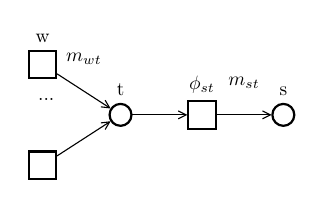
\begin{tikzpicture}
      \begin{scope}[scale=0.7, shift={(-3,-4.5)}, every node/.append style={transform shape}, local bounding box=mmrfToy]
        \tikzstyle{enode} = [thick, draw=black, circle, inner sep = 4pt, align=center]
        \tikzstyle{nnode} = [thick, rectangle, rounded corners = 0pt, minimum size = 0.5cm,draw,inner sep = 2pt]
        
        \node[enode, label=above:{t}] (t) at (0 ,0) {};
        \node[nnode, label=above:{$\phi_{st}$}, right=of t] (phiSt) {};
        \node[enode, label=above:{s}, right=of phiSt] (s) {};
        \node[nnode, label=above:{w}, above left= 0.5 and 1 of t] (w) {};
        \node[label=above:{...}, left= of t] (w1) {};
        \node[nnode, below left= 0.5 and 1 of t] (w2) {};

        \draw[->] (w) -- node[midway,above=1em]{$m_{wt}$} (t);
        \draw[->] (w2) to (t);
        \draw[->] (t) to (phiSt);
        \draw[->] (phiSt) to node[midway,above=1em]{$m_{st}$} (s);

      \end{scope}
    \end{tikzpicture}
  \end{columns}
  \begin{align*}
    \underbrace{{m}^{\mathrm{new}}_{ts}(x_s)}_{\text{new msg. to s}} \propto
    \underbrace{m_{ts}(x_s)^{1-\alpha_{ts}}}_{\text{old msg. to s}} \bigg[\sum_{x_t} \phi_{ts}(x_t, x_s)^{\alpha_{ts}} \underbrace{{m}_{st}(x_t)^{1-\alpha_{ts}}}_{\text{old msg. to t}} \underbrace{{\phi}_t(x_t) \prod_{w\in \Nn(t)\backslash s}m_{wt}(x_t)}_{\text{msg. from variable node $t$ to factor $\phi_{st}$}} \bigg].
  \end{align*}
  
  \centering
  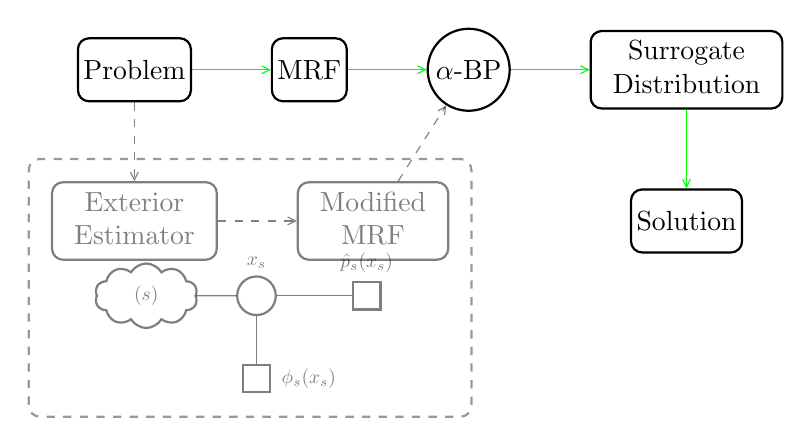
\begin{tikzpicture}
    \tikzstyle{enode} = [thick, draw, circle, inner sep = 2pt, align=center]
    \tikzstyle{nnode} = [thick, rectangle, rounded corners = 4pt, minimum size = 0.8cm,draw,inner sep = 2pt]
    \tikzstyle{cnode} = [thick, cloud, draw, cloud puffs=10, cloud puff arc=120, aspect=2, inner ysep=4pt]

    \begin{scope}
      
      \node[nnode] (Problem) at (-4, 0) {Problem};
      \node[nnode, right= of Problem] (pGraph) 
      {MRF
      };
      \node[enode, right=of pGraph] (alpha) {$\alpha$-BP};
      \node[nnode, right=of alpha] (surrogate) {
        \begin{tabular}{c}
          Surrogate \\
          Distribution
        \end{tabular}};
      \node[nnode, below=of surrogate] (sol) {Solution};

      \node[nnode, below=of Problem, opacity=0.5] (ext) {\begin{tabular}{c}Exterior \\ Estimator\end{tabular}};
      \node[nnode, right=of ext, opacity=0.5] (mmrf) {\begin{tabular}{c}Modified\\MRF\end{tabular}};
      

      \draw[green,->] (Problem) to (pGraph);
      \draw[green,->] (pGraph) to (alpha);
      \draw[green,->] (alpha) to (surrogate);
      \draw[green,->] (surrogate) to (sol);
      \draw[dashed, ->, opacity=0.5] (Problem) to (ext);
      \draw[dashed, ->, opacity=0.5] (ext) to (mmrf);
      \draw[dashed, ->, opacity=0.5] (mmrf) to (alpha);

    \end{scope}
    \begin{scope}[scale=0.7, shift={(-3.5,-4.1)}, every node/.append style={transform shape}, local bounding box=mmrfToy, opacity=0.5]
      \tikzstyle{enode} = [thick, draw=black, circle, inner sep = 4pt, minimum size = 0.7cm, align=center]
      \tikzstyle{nnode} = [thick, rectangle, rounded corners = 0pt, minimum size = 0.5cm,draw,inner sep = 2pt]
      \tikzstyle{cnode} = [thick, cloud, draw,cloud puffs=10, cloud puff arc=120, aspect=2, inner ysep=4pt]

      \node[cnode] (paik) at (-2, 0) {$\Nn(s)$};
      \node[enode] (xi) at (0 ,0) {};
      \node[] at ($(xi) + (0,0.6)$) {$x_s$};

      \node[nnode] (fi) at (0 , -1.5) {};
      \node[] at ($(fi) + (0.95, 0)$) {$\phi_s(x_s)$};

      \node[nnode] (pi) at (2, 0) {};
      \node[] at ($(pi) + (0, 0.6)$) {$\hat{p}_s(x_s)$};
      % connections
      \draw[-] (xi) to (fi);
      \draw[-] (xi) to (pi);
      \draw[-] (xi) to (paik);
    \end{scope}
    \node[nnode, fit=(mmrf)(ext)(mmrfToy), inner sep=8pt, dashed,draw=black!40] {};
  \end{tikzpicture}
\end{frame}

\begin{frame}
  \begin{columns}
    \column{0.5\textwidth}
    Updating message via $\alpha$-BP:
    \column{0.5\textwidth}

    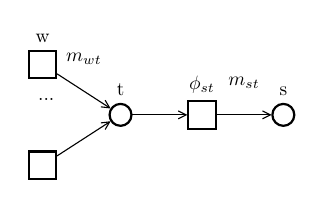
\begin{tikzpicture}
      \begin{scope}[scale=0.7, shift={(-3,-4.5)}, every node/.append style={transform shape}, local bounding box=mmrfToy]
        \tikzstyle{enode} = [thick, draw=black, circle, inner sep = 4pt, align=center]
        \tikzstyle{nnode} = [thick, rectangle, rounded corners = 0pt, minimum size = 0.5cm,draw,inner sep = 2pt]
        
        \node[enode, label=above:{t}] (t) at (0 ,0) {};
        \node[nnode, label=above:{$\phi_{st}$}, right=of t] (phiSt) {};
        \node[enode, label=above:{s}, right=of phiSt] (s) {};
        \node[nnode, label=above:{w}, above left= 0.5 and 1 of t] (w) {};
        \node[label=above:{...}, left= of t] (w1) {};
        \node[nnode, below left= 0.5 and 1 of t] (w2) {};

        \draw[->] (w) -- node[midway,above=1em]{$m_{wt}$} (t);
        \draw[->] (w2) to (t);
        \draw[->] (t) to (phiSt);
        \draw[->] (phiSt) to node[midway,above=1em]{$m_{st}$} (s);

      \end{scope}
    \end{tikzpicture}
  \end{columns}
  
  \begin{align*}
    \underbrace{{m}^{\mathrm{new}}_{ts}(x_s)}_{\text{new msg. to s}} \propto
    \underbrace{m_{ts}(x_s)^{1-\alpha_{ts}}}_{\text{old msg. to s}} \bigg[\sum_{x_t} \phi_{ts}(x_t, x_s)^{\alpha_{ts}} \underbrace{{m}_{st}(x_t)^{1-\alpha_{ts}}}_{\text{old msg. to t}} \underbrace{{\phi}_t(x_t) \prod_{w\in \Nn(t)\backslash s}m_{wt}(x_t)}_{\text{msg. from variable node $t$ to factor $\phi_{st}$}} \bigg].
  \end{align*}
  \centering
  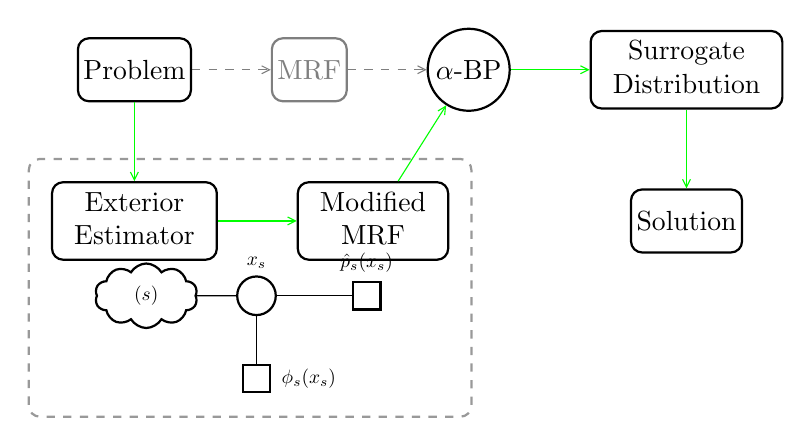
\begin{tikzpicture}
    \tikzstyle{enode} = [thick, draw, circle, inner sep = 2pt, align=center]
    \tikzstyle{nnode} = [thick, rectangle, rounded corners = 4pt, minimum size = 0.8cm,draw,inner sep = 2pt]
    \tikzstyle{cnode} = [thick, cloud, draw, cloud puffs=10, cloud puff arc=120, aspect=2, inner ysep=4pt]

    \begin{scope}
      
      \node[nnode] (Problem) at (-4, 0) {Problem};
      \node[nnode, right= of Problem, opacity=0.5] (pGraph) 
      {MRF
      };
      \node[enode, right=of pGraph] (alpha) {$\alpha$-BP};
      \node[nnode, right=of alpha] (surrogate) {
        \begin{tabular}{c}
          Surrogate \\
          Distribution
        \end{tabular}};
      \node[nnode, below=of surrogate] (sol) {Solution};

      \node[nnode, below=of Problem] (ext) {\begin{tabular}{c}Exterior \\ Estimator\end{tabular}};
      \node[nnode, right=of ext] (mmrf) {\begin{tabular}{c}Modified\\MRF\end{tabular}};
      

      \draw[dashed,->,opacity=0.5] (Problem) to (pGraph);
      \draw[dashed,->,opacity=0.5] (pGraph) to (alpha);
      \draw[green,->] (alpha) to (surrogate);
      \draw[green,->] (surrogate) to (sol);
      \draw[green, ->] (Problem) to (ext);
      \draw[green, ->] (ext) to (mmrf);
      \draw[green, ->] (mmrf) to (alpha);

    \end{scope}
    \begin{scope}[scale=0.7, shift={(-3.5,-4.1)}, every node/.append style={transform shape}, local bounding box=mmrfToy]
      \tikzstyle{enode} = [thick, draw=black, circle, inner sep = 4pt, minimum size = 0.7cm, align=center]
      \tikzstyle{nnode} = [thick, rectangle, rounded corners = 0pt, minimum size = 0.5cm,draw,inner sep = 2pt]
      \tikzstyle{cnode} = [thick, cloud, draw,cloud puffs=10, cloud puff arc=120, aspect=2, inner ysep=4pt]

      \node[cnode] (paik) at (-2, 0) {$\Nn(s)$};
      \node[enode] (xi) at (0 ,0) {};
      \node[] at ($(xi) + (0,0.6)$) {$x_s$};

      \node[nnode] (fi) at (0 , -1.5) {};
      \node[] at ($(fi) + (0.95, 0)$) {$\phi_s(x_s)$};

      \node[nnode] (pi) at (2, 0) {};
      \node[] at ($(pi) + (0, 0.6)$) {$\hat{p}_s(x_s)$};
      % connections
      \draw[-] (xi) to (fi);
      \draw[-] (xi) to (pi);
      \draw[-] (xi) to (paik);
    \end{scope}
    \node[nnode, fit=(mmrf)(ext)(mmrfToy), inner sep=8pt, dashed,draw=black!40] {};
  \end{tikzpicture}
  
\end{frame}

\begin{frame}{Insights of $\alpha$-BP}
  \begin{columns}
    \column{0.5\textwidth}
    \begin{block}{\small Connection to standard BP}
      \begin{itemize}[label=$\bullet$]
      \item $\alpha \rightarrow 0$ 
      \item $\alpha$-divergence reduce KL-divergence
      \item Update rule of $\alpha$-BP reduces to ${m}^{\text{new}}_{ts}(x_s) \propto \sum_{x_t} \phi_{st}(x_s, x_t) {\phi}_t(x_t) \prod_{w\in \Nn(t)\backslash s}m_{wt}(x_t)$, which is standard BP update rule
        
      \end{itemize}
    \end{block}
    \column{0.45\textwidth}
    \begin{block}{\small Convergence}
      For an arbitrary pairwise Markov random field over binary variables,
      if the largest singular value of matrix $\bm{M}(\bm{\alpha}, \bm{\theta})$ is less than one,
      $\alpha$-BP converges to a fixed point. The associated fixed point is unique.
      \vfill
      {\tiny See Corollary 3.1 for relaxed condition where singular value computation is avoided.}
    \end{block}
  \end{columns}
  \vskip 0.5cm
  \begin{block}{\small What does that mean}
    \begin{itemize}[label=$\bullet$]
    \item You can safely use $\alpha$-BP as an alternative to (loopy) BP
    \item You can use matrix $\bm{M}$ to check if you are guaranteed to get stable solution from $\alpha$-BP
    \end{itemize}
  \end{block}
  \let\thefootnote\relax\footnotetext{\tiny
    \vskip -0.2cm
    \begin{columns}
      \column{0.5\textwidth}
      For binary, symmetric log-potentials 
      \begin{align*}
        \phi_{st}(x_s, x_t) &= \exp\left\{ \theta_{st}(x_s, x_t)\right\}, \nonumber \\
        \phi_{s}(x_s) &= \exp\left\{ \theta_{s}(x_s) \right\}.
      \end{align*}
      \column{0.5\textwidth}
      Matrix $\bm{M}(\bm{\alpha}, \bm{\theta})$, size $\abs{\vec{\Ee}} \times \abs{\vec{\Ee}}$, indexed by directed edges $(t\rightarrow s)$, as
      \begin{align*}
        M_{(t\rightarrow s), (u \rightarrow v)} =
        \begin{cases}
          \abs{ 1 - \alpha_{ts}}, &\quad u=t, v=s, \\
          \abs{ 1 - \alpha_{ts}} \tanh \abs{\alpha_{ts} \theta_{ts}}, & \quad u = s, v =t, \\
          \tanh\abs{\alpha_{ts} \theta_{ts}}, & \quad u \in \Nn(t)\backslash s, v = t, \\
          0, & \quad \mathrm{otherwise}.
        \end{cases}
      \end{align*}
    \end{columns}
  }
\end{frame}
\begin{frame}{Some Numerical Results}
  
  \graphicspath{{../source/chapter3/}}
  \begin{columns}
    \column{0.5\textwidth}
    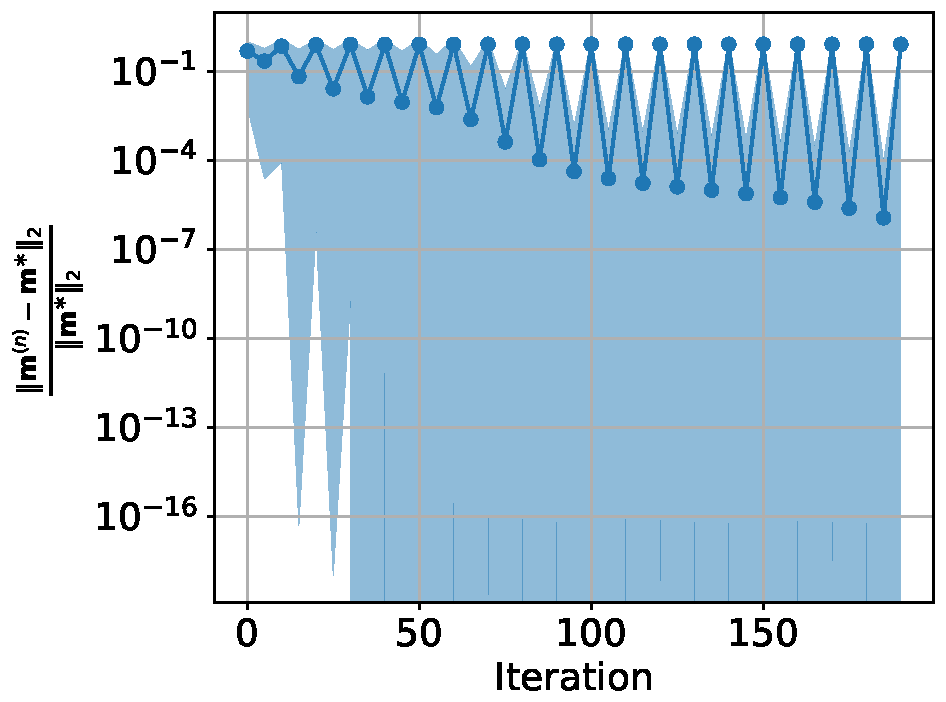
\includegraphics[width=0.8\columnwidth]{figures/converge/converge_erp0_4_alpha_1_stn_0_5_vs_filter_false_crop.pdf}
    \column{0.5\textwidth}
    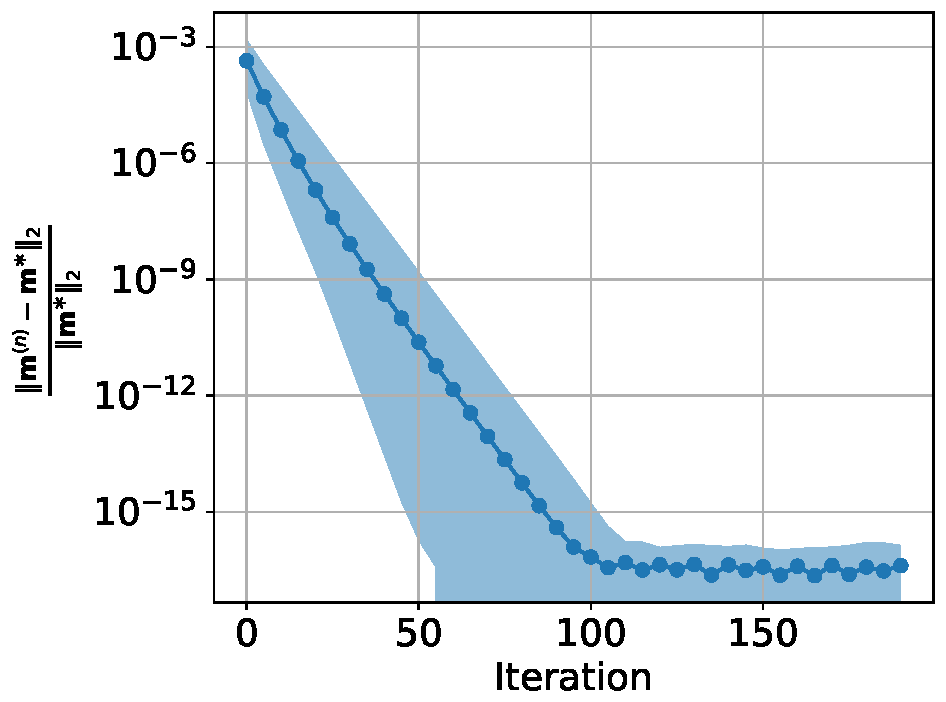
\includegraphics[width=0.8\columnwidth]{figures/converge/converge_erp0_2_alpha_0_5_stn_0_1_vs_filter_true-crop.pdf}
  \end{columns}
  \centering
  {\tiny Numerical illustration of convergence, with normalized error ${\normd{\bm{m}^{(n)}-\bm{m}^{\ast}}}/{\normd{\bm{m}^{\ast}}}$ versus the number of iterations. Number of nodes $N=16$. Blue region denotes the range from minimum to maximum of the normalized error of $100$ graph realizations, whereas the curve stands for mean error of the $100$ realized graphs. }
  \vskip -0.2cm
  \begin{columns}
    \column{0.5\textwidth}
    \begin{center}
      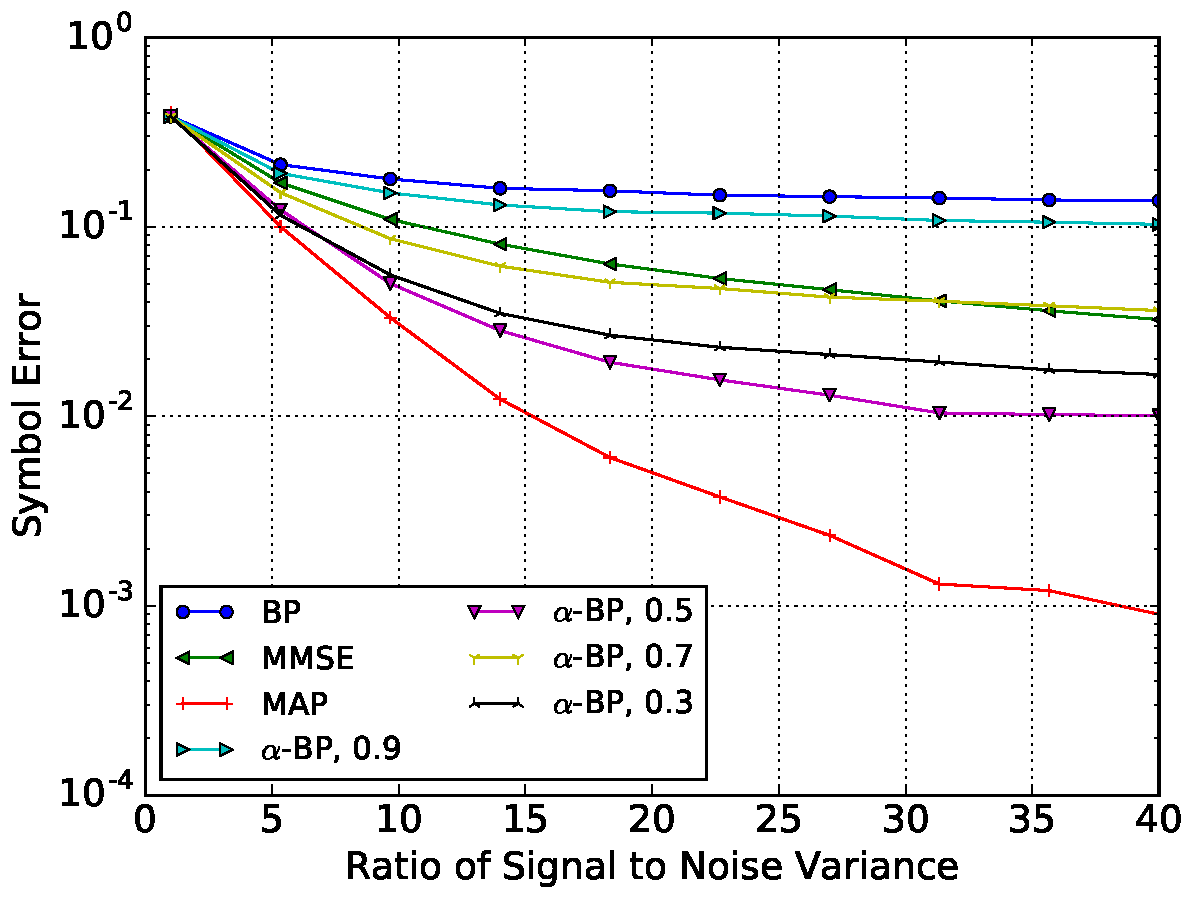
\includegraphics[width=0.8\columnwidth]{figures/alpha_compare_crop.pdf}
    \end{center}
    \column{0.5\textwidth}
    \centering
    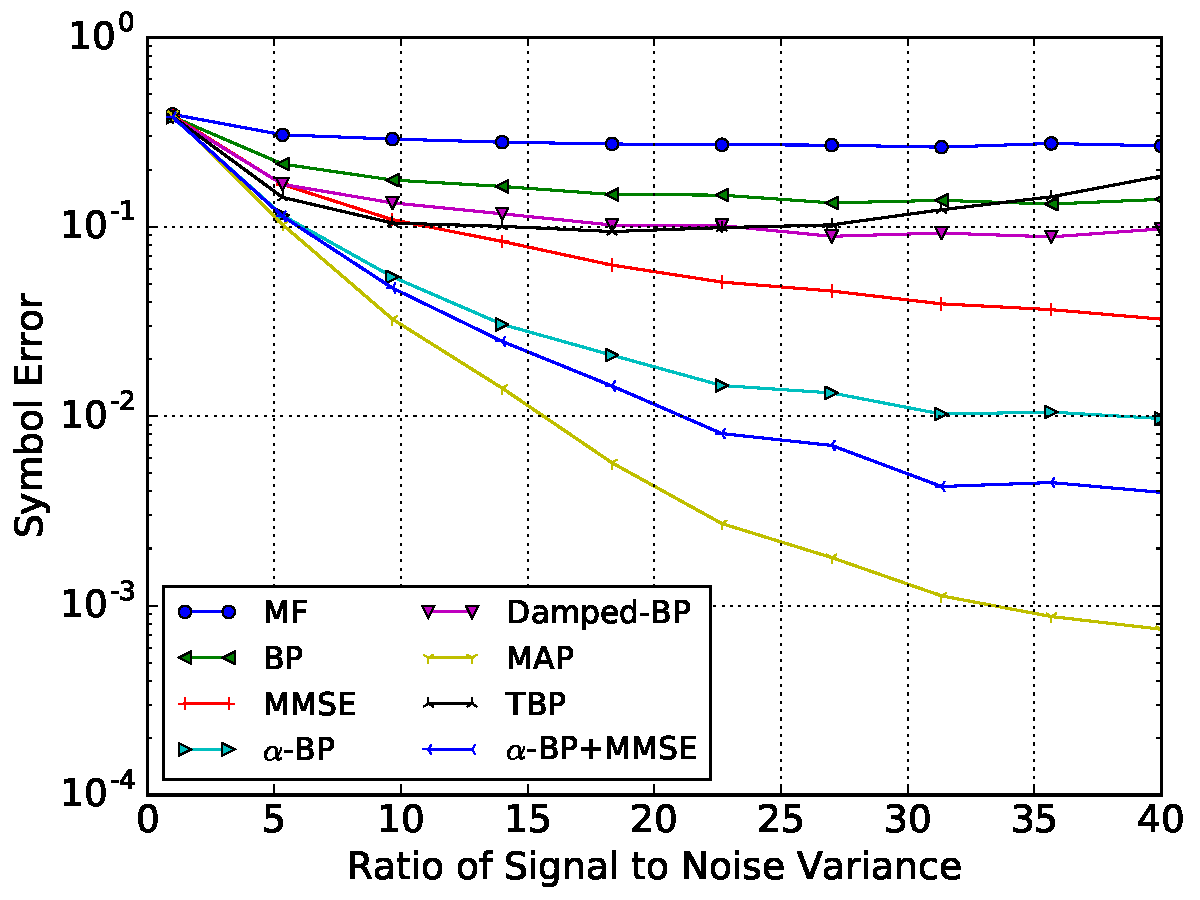
\includegraphics[width=0.8\columnwidth]{figures/tbp/mf_tbp_compare.pdf}
  \end{columns}
  \centering
  {\tiny Numerical results of $\alpha$-BP: symbol error of MIMO detection.}

\end{frame}


% \subsection{GraphNet}

% \begin{frame}{Learn the message update rule by NN}
%   An end-to-end learning process: Factor graph $\rightarrow$ converted graph representation $\rightarrow$ GNN $\rightarrow$ Output
%   \begin{figure}
%     \centerline{\includegraphics[scale=0.3]{images/gnn.png}}
%   \end{figure}
%   \begin{itemize}[label=$\bullet$]
%   \item sum-product update rule (in BP) $\rightarrow$ NN, to learn
%   \item pseudo probability (belief aggregation) $\rightarrow$ NN, to learn
%   \item end-to-end learning that requires true marginal probability, which BP, GPB and mean field do no require
%   \end{itemize}
%   \let\thefootnote\relax\footnotetext{\tiny For related methods, see:\\
%   Heess et al, Learning to Pass Expectation Propagation Messages\\
%   Yoon, et al, 2019, Inference in Probabilistic Graphical Models by Graph Neural Networks\\
%   Gilmer, et al, 2017, Neural message passing for quantum chemistry.\\
%   Battaglia, et al, 2018, Relational inductive biases, deep learning, and graph networks
% }
% \end{frame}

% \subsection{AutoEncoder}

% \begin{frame}
%   {Variational Auto-encoder}
%   \onslide<1->{
%   \begin{itemize}[label=$\bullet$]
%   \item Simplification on structures \\
%     \begin{tikzpicture}
%       \tikzstyle{enode} = [thick, draw=black, circle, inner sep = 2pt,  align=center]
%       \tikzstyle{nnode} = [thick, rectangle, rounded corners = 2pt, minimum size = 0.5cm,draw,inner sep = 2pt]
%       \tikzstyle{fnode} = [draw=blue, ellipse, inner sep = 1pt]
%       \tikzstyle{fnoder} = [draw=red, ellipse, inner sep = 0.0pt, rotate=-20]

%       \begin{scope}[scale=0.5]
%         \node[enode] (x1) at (-1.5, 1) {$x_1$};
%         \node[enode] (x2) at (-1.5, -1) {$x_2$};
%         \node[enode] (x3) at (0.5, 1) {$x_3$};
%         \node[enode] (x4) at (0.5, -1) {$x_4$};
%         \draw (x1) -- (x2)
%         (x1) -- (x3)
%         (x4) -- (x3)
%         (x4) -- (x2)
%         ;
%       \end{scope}
%       \begin{scope}[scale=0.5, xshift=5cm]
%         \node[enode] (x1) at (-1.5, 1) {$x_1$};
%         \node[enode] (x2) at (-1.5, -1) {$x_2$};
%         \node[enode] (x3) at (0.5, 1) {$x_3$};
%         \node[enode] (x4) at (0.5, -1) {$x_4$};
%       \end{scope}

%     \end{tikzpicture}
%   }
%     \onslide<2->{
%   \item Care about only a certain set of variables \\
%     \begin{tikzpicture}
%       \tikzstyle{enode} = [thick, draw=black, circle, inner sep = 2pt,  align=center]
%       \tikzstyle{nnode} = [thick, rectangle, rounded corners = 2pt, minimum size = 0.5cm,draw,inner sep = 2pt]
%       \tikzstyle{fnode} = [draw=blue, ellipse, inner sep = 3pt]


%       \begin{scope}[scale=0.5]
%         \node[enode] (x1) at (-1.5, 1) {$x_1$};
%         \node[enode] (x2) at (-1.5, -1) {$x_2$};
%         \node[fnode, fit=(x1)(x2)] (xo){$\bm{x}_O$};
%       \end{scope}
%       \begin{scope}[scale=0.5, xshift=5cm]
%         \node[enode] (x3) at (0.5, 1) {$x_3$};
%         \node[enode] (x4) at (0.5, -1) {$x_4$};
%         \node[fnode, fit=(x3)(x4)] (xu) {$\bm{x}_U$};
%       \end{scope}

%     \end{tikzpicture}
%   }
%     \onslide<3->{
%   \item Amortizing the probabilities of interests and learn their parameters by sampling
%     \begin{tikzpicture}
%       \tikzstyle{enode} = [thick, draw=black, circle, inner sep = 2pt,  align=center]
%       \tikzstyle{nnode} = [thick, rectangle, rounded corners = 2pt, minimum size = 0.5cm,draw,inner sep = 2pt]
%       \tikzstyle{fnode} = [draw=blue, ellipse, inner sep = 3pt]

%       \node[fnode] (xo) at (0,0){$\bm{x}_O$};
%       \node[fnode] (xu) at (3,0) {$\bm{x}_U$};
%       \node[fnode] (hxo) at (6,0){$\hat{\bm{x}}_O$};
%       \draw[->] (xo) to node[above]{$q(\bm{x}_U|\bm{x}_O)$} (xu);
%       \draw[->](xu) to node[above]{${{p}(\bm{x}_O| \bm{x}_U; \bm{\theta})}$}(hxo);
%     \end{tikzpicture}

%     with the \textbf{variational free energy $F_V$ rewritten as}
%     \begin{equation*}
%       F_V(q, \bm{\theta}) = \EE_{q(\bm{x}_U|\bm{x}_O)}\left[ \log{{p}(\bm{x}_O| \bm{x}_U; \bm{\theta})} + \log{{p}(\bm{x}_U; \bm{\theta})} \right] + H({q(\bm{x}_U|\bm{x}_O)}),
%     \end{equation*}
%   }
%   \end{itemize}
% \end{frame}
\subsection{RENN}
{ \setbeamercolor{background canvas}{bg=hl_bg}
  \setbeamercolor{normal text}{fg=hl_fg}
  \setbeamercolor{frametitle}{fg=hl_fg}
  \begin{frame}[label=current]
    \usebeamercolor[fg]{normal text}
    \begin{center}
      {
        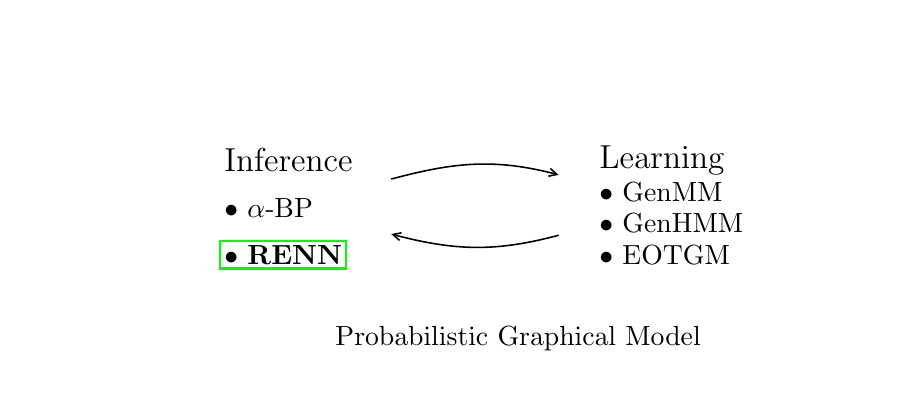
\begin{tikzpicture}
          \tikzstyle{cnode} = [thick, draw=white, ellipse, inner sep = 2pt,  align=center]
          \tikzstyle{fnode} = [thick, draw=white, ellipse, inner sep = 10pt,  align=center]
          \tikzstyle{rnode} = [thick, rectangle, inner sep = 1.5pt,  align=left]
          \node[rnode] (inf) at (-2, 0) {\large Inference};
          \node[rnode, below = 0.6cm of inf.west, anchor=west] (abp) {$\bullet$ $\alpha$-BP};
          \node[rnode, below = 1.2cm of inf.west, anchor=west, draw=green] (renn) {$\bullet$ \textbf{RENN}};
          \node[cnode, fit=(abp)(inf)(renn)] (infn) {};
          
          \node[rnode, right = 3 of inf] (lern) {\large Learning};
          \node[rnode, below = 0.4 of lern.west, anchor=west] (genmm) {$\bullet$ GenMM};
          \node[rnode, below = 0.8 of lern.west, anchor=west] (genhmm) {{$\bullet$} GenHMM};
          \node[rnode, below = 1.2 of lern.west, anchor=west] (lfree) {{$\bullet$} EOTGM};
          \node[cnode, fit=(lern)(genmm)(genhmm)(lfree)] (learn) {};

          \node[fnode, fit=(infn)(lern)] (box) {};

          
          \node[below right = 0.5 and -0.5 of infn] {{Probabilistic} Graphical Model};
          \draw[->,line width=0.2mm] (infn) to[out=15, in=165] (learn);
          \draw[->,line width=0.2mm] (learn) to[out=195, in=-15] (infn);
        \end{tikzpicture}
      }
    \end{center}
    
  \end{frame}
}

\begin{frame}[label=current]{Continuing: What is the state of $x$?}
  \framesubtitle{Yedidia, Freeman, Weiss: A step to generalization}
  \textbf{Message among variables \& factors $\rightarrow$ message among regions}
  \textcolor{red}{Maybe I should combine this slide to the next one}
  \begin{columns}
    \column{0.6\textwidth}
    \centering
    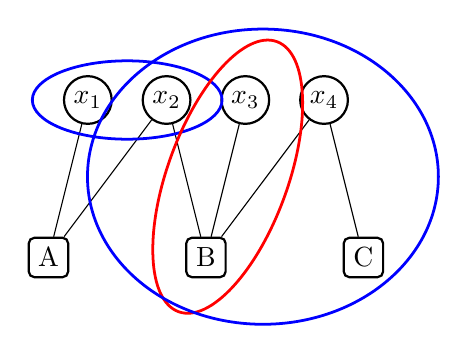
\begin{tikzpicture}[scale=1, every node/.append style={transform shape}]
      % \tikzstyle{enode} = [thick, draw=blue, circle, inner sep = 3pt,
      % align=center]
      \tikzstyle{enode} = [thick, draw=black, circle, inner sep = 2pt,  align=center]
      \tikzstyle{nnode} = [thick, rectangle, rounded corners = 2pt, minimum size = 0.5cm,draw,inner sep = 2pt]
      \tikzstyle{fnode} = [draw=blue, ellipse, inner sep = 1pt]
      \tikzstyle{fnoder} = [draw=red, ellipse, inner sep = 0.0pt, rotate=-20]


      \node[enode] (x1) at (-1.5, 1) {$x_1$};
      \node[enode] (x2) at (-0.5, 1) {$x_2$};
      \node[enode] (x3) at (0.5, 1) {$x_3$};
      \node[enode] (x4) at (1.5, 1) {$x_4$};

      \node[nnode] (a) at (-2,-1) {A};
      \node[nnode] (b) at (0,-1) {B};
      \node[nnode] (c) at (2,-1) {C};

      \draw[-] (a) to (x1);
      \draw[-] (a) to (x2);
      \draw[-] (b) to (x2);
      \draw[-] (b) to (x3);
      \draw[-] (b) to (x4);
      \draw[-] (c) to (x4);
      
      \node[fnode, fit=(x1)(x2)] (box) {};
      \node[fnoder, fit=(x3)(b)] (box) {};

      \node[fnode, fit=(x2)(x3)(x4)(b)(c)] (box) {};
    \end{tikzpicture}
    \column{0.4\textwidth}
    \begin{itemize}[label=\textbullet]
    \item Blue region: valid region
    \item Red region: invalid region
    \end{itemize}
  \end{columns}
  
  
  % A region in a region graph acts as a node, and there are directed edges between regions which are defined according to specific rules. Formally, a region graph is defined as follows:

  % A \textit{region graph} is  a directed graph $\Gg_R(\Rr, \Ee)$, where each vertex $R \in \Rr$ is defined as the joint set of variable and factor nodes in this region, i.e., $R = \left\{ i \in V_R, a \in A_R | i \in \Vv, a \in \Ff \right\}$. Each edge $e \in \Ee$ in $\Gg_R$ is directed from $R_p$ to $R_c$ such that $R_c \subset R_p$. 

  Generalized belief propagation (GBP) generalizes loopy BP
  \begin{itemize}[label={$\bullet$}]
  \item usual better approximation than LBP
  \item higher complexity
  \item sensitive to scheduling of region messages
  \end{itemize}
  Corresponding to minimization of approximated \textbf{variational free energy $F_v(b)$  with trial $b$ including $\{b_R\}$}.
  \let\thefootnote\relax\footnotetext{\tiny
    \vskip -0.2cm
    A \textit{region} $R$ is a set $V_R$ of variables nodes and a set $A_R$ of factor nodes, such that if a factor node '$a$' belongs to $A_R$, all the variables nodes neighboring $a$ are in $V_R$.
  }
\end{frame}

\begin{frame}[label=current]{An Toy Example of Region Graphs}
  Factor graph representation of MRF (2-by-3 grid) with factor nodes.\\
  MRF $\rightarrow$ region graph:\\
  \vskip 0.5cm
  \begin{columns}
    \centering
    \column{0.7\textwidth}
    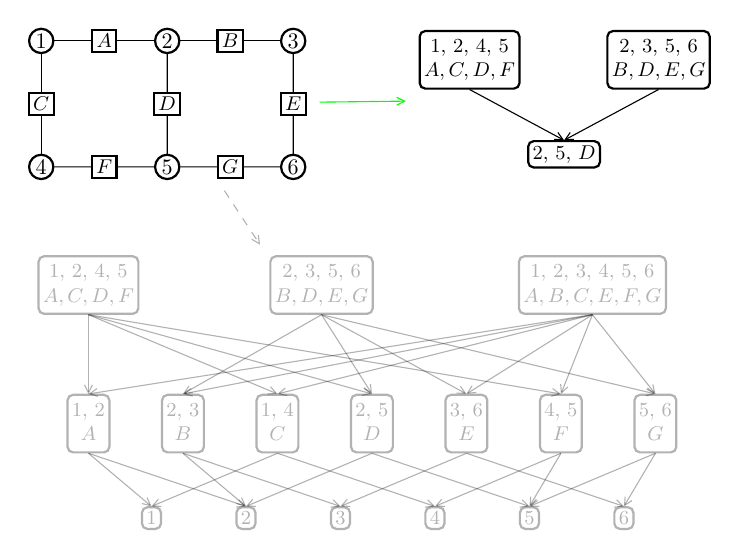
\begin{tikzpicture}
      \tikzstyle{cnode} = [thick, draw=black, circle, inner sep = 1pt,  align=center]
      \tikzstyle{nnode} = [thick, rectangle, rounded corners = 0pt,draw,inner sep = 2pt]

      %%%%%%%%%%%%%%%%%%%%%%%%%%%%%% 
      %% The 2-by-3 factor graph
      %%%%%%%%%%%%%%%%%%%%%%%%%%%%%% 
      \begin{scope}[scale=0.8, every node/.append style={transform shape}, local bounding box=grid]
        \node[cnode] (x1) at (0,0) {1};
        \node[cnode] (x2) at (2,0) {2};
        \node[cnode] (x3) at (4,0) {3};

        \node[cnode] (x4) at (0,-2) {4};
        \node[cnode] (x5) at (2,-2) {5};
        \node[cnode] (x6) at (4,-2) {6};

        \node[nnode] (fa) at (1,0) {\small$A$};
        \node[nnode] (fb) at (3,0) {\small$B$};

        \node[nnode] (fc) at (0,-1) {\small$C$};
        \node[nnode] (fd) at (2,-1) {\small$D$};
        \node[nnode] (fe) at (4,-1) {\small$E$};
        
        \node[nnode] (ff) at (1,-2) {\small$F$};
        \node[nnode] (fg) at (3,-2) {\small$G$};


        \draw[-] (x1) -- (fa);
        \draw[-] (x1) -- (fc);

        \draw[-] (x2) -- (fa);
        \draw[-] (x2) -- (fb);
        \draw[-] (x2) -- (fd);

        \draw[-] (x3) -- (fb);
        \draw[-] (x3) -- (fe);

        \draw[-] (x4) -- (fc);
        \draw[-] (x4) -- (ff);

        \draw[-] (x5) -- (fd);
        \draw[-] (x5) -- (ff);
        \draw[-] (x5) -- (fg);

        \draw[-] (x6) -- (fe);
        \draw[-] (x6) -- (fg);

      \end{scope}
      %%%%%%%%%%%%%%%%%%%%%%%%%%%%%% 
      %% The 2-layer region graph
      %%%%%%%%%%%%%%%%%%%%%%%%%%%%%% 
      \begin{scope}[scale=0.8, every node/.append style={transform shape}, xshift=6.8cm, yshift=-0.3cm, local bounding box=rg2]
        \tikzstyle{rnode} = [thick, rectangle, rounded corners = 2pt,minimum size = 0.0cm,draw,inner sep = 2pt]
        \node[rnode] (r01) at (0,0) {\small \begin{tabular}[x]{@{}c@{}}1, 2, 4, 5 \\ $A,C,D,F$ \end{tabular}};
        \node[rnode] (r02) at (3,0) {\small \begin{tabular}[x]{@{}c@{}}2, 3, 5, 6\\ $B,D,E,G$ \end{tabular}};
        \node[rnode] (r11) at (1.5, -1.5) {\small 2, 5, $D$};

        \draw[->] (r01.south) -- (r11.north);
        \draw[->] (r02.south) -- (r11.north);
      \end{scope}

      %%%%%%%%%%%%%%%%%%%%%%%%%%%%%% 
      %% The 3-layer region graph
      %%%%%%%%%%%%%%%%%%%%%%%%%%%%%% 
      \begin{scope}[xshift=0.6cm, yshift=-3.1cm,scale=0.8, every node/.append style={transform shape},local bounding box=rg3, opacity=0.3]
        \tikzstyle{rnode} = [thick, rectangle, rounded corners = 2pt,minimum size = 0.0cm,draw,inner sep = 2pt]
        \node[rnode] (r01) at (0,0) {\small\begin{tabular}[x]{@{}c@{}}1, 2, 4, 5 \\ $A,C,D,F$ \end{tabular}};
        \node[rnode] (r02) at (3.7,0) {\small\begin{tabular}[x]{@{}c@{}}2, 3, 5, 6\\ $B,D,E,G$ \end{tabular}};
        \node[rnode] (r03) at (8,0) {\small\begin{tabular}[x]{@{}c@{}}1, 2, 3, 4, 5, 6\\ $A,B,C,E,F,G$ \end{tabular}};
        \begin{scope}[yshift=-0.2cm]
          \node[rnode] (r11) at (0, -2.0) {\small\begin{tabular}[x]{@{}c@{}}1, 2\\ $A$ \end{tabular}};
          \node[rnode] (r12) at (1.5, -2.0) {\small\begin{tabular}[x]{@{}c@{}}2, 3\\ $B$ \end{tabular}};
          \node[rnode] (r13) at (3, -2.0) {\small\begin{tabular}[x]{@{}c@{}}1, 4\\ $C$ \end{tabular}};
          \node[rnode] (r14) at (4.5, -2.0) {\small\begin{tabular}[x]{@{}c@{}}2, 5\\ $D$ \end{tabular}};
          \node[rnode] (r15) at (6, -2.0) {\small\begin{tabular}[x]{@{}c@{}}3, 6\\ $E$ \end{tabular}};
          \node[rnode] (r16) at (7.5, -2.0) {\small\begin{tabular}[x]{@{}c@{}}4, 5\\ $F$ \end{tabular}};
          \node[rnode] (r17) at (9, -2.0) {\small\begin{tabular}[x]{@{}c@{}}5, 6\\ $G$ \end{tabular}};

          \begin{scope}[yshift=0.5cm]
            \node[rnode] (r21) at (1, -4) {\small 1};
            \node[rnode] (r22) at (2.5, -4) {\small 2};
            \node[rnode] (r23) at (4, -4) {\small 3};
            \node[rnode] (r24) at (5.5, -4) {\small 4};
            \node[rnode] (r25) at (7, -4) {\small 5};
            \node[rnode] (r26) at (8.5, -4) {\small 6};
          \end{scope}
        \end{scope}
        % edge level0 to level1
        \draw[->] (r01.south) -- (r11.north);
        \draw[->] (r03.south) -- (r11.north);

        \draw[->] (r02.south) -- (r12.north);
        \draw[->] (r03.south) -- (r12.north);

        \draw[->] (r01.south) -- (r13.north);
        \draw[->] (r03.south) -- (r13.north);

        \draw[->] (r01.south) -- (r14.north);
        \draw[->] (r02.south) -- (r14.north);

        \draw[->] (r02.south) -- (r15.north);
        \draw[->] (r03.south) -- (r15.north);

        \draw[->] (r01.south) -- (r16.north);
        \draw[->] (r03.south) -- (r16.north);

        \draw[->] (r02.south) -- (r17.north);
        \draw[->] (r03.south) -- (r17.north);

        % edge level1 to level2
        \draw[->] (r11.south) -- (r21.north);
        \draw[->] (r13.south) -- (r21.north);

        \draw[->] (r11.south) -- (r22.north);
        \draw[->] (r12.south) -- (r22.north);
        \draw[->] (r14.south) -- (r22.north);


        \draw[->] (r12.south) -- (r23.north);
        \draw[->] (r15.south) -- (r23.north);

        \draw[->] (r13.south) -- (r24.north);
        \draw[->] (r16.south) -- (r24.north);

        \draw[->] (r14.south) -- (r25.north);
        \draw[->] (r16.south) -- (r25.north);
        \draw[->] (r17.south) -- (r25.north);

        \draw[->] (r15.south) -- (r26.north);
        \draw[->] (r17.south) -- (r26.north);
      \end{scope}
      \draw[green, ->, shorten >=5pt, shorten <=5pt] (grid) -- (rg2);
      \draw[opacity=0.3, dashed, ->, shorten >=5pt, shorten <=5pt] (grid) -- (rg3);
      

    \end{tikzpicture}
    \column{0.3\textwidth}
    \begin{itemize}[label=\textbullet]
    \item Clustering nodes
    \item Valid regions
    \item Energy Calculated per region
    \item Msg. Scheduling
    \item ...
    \item See Section 4.1
      
    \end{itemize}
  \end{columns}

  
\end{frame}
\begin{frame}[label=current]{RENN: Region-based Energy Neural Network}
  The \textbf{region-based free energy} of a region graph is
  \begin{equation*}
    F_R(\Bb; \bm{\theta}) = \sum_{R\in \Rr} \underbrace{c_R}_{\text{Counting number}} \sum_{\bm{x}_R}\underbrace{b_R(\bm{x}_R)}_{\text{Belief on region R}} (\underbrace{E_R(\bm{x}_R; \bm{\theta}_R)}_{\text{Region average energy}} + \ln{b_R}(\bm{x}_R)),
  \end{equation*}
  \begin{itemize}[label=$\bullet$]
  \item counting number: balance the contribution of each region
  \item region average energy: $- \sum_{a\in A_R} \ln{\phi_a(\bm{x}_a; \bm{\theta}_a)}$
  \end{itemize}
  
  
  
  \begin{columns}
    \column{0.3\textwidth}
    \centering
    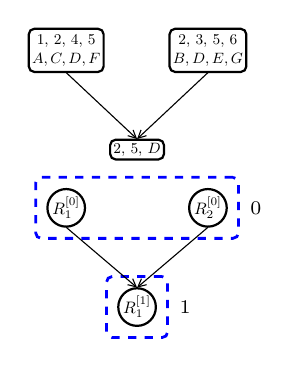
\begin{tikzpicture}
      
      \tikzstyle{cnode} = [thick, draw=black, circle, inner sep = 1pt,  align=center]
      \tikzstyle{nnode} = [thick, rectangle, rounded corners = 0pt,draw,inner sep = 2pt]
      
      \begin{scope}[xshift=0cm, scale=0.6, every node/.append style={transform shape}, local bounding box=rg2]
        \tikzstyle{rnode} = [thick, rectangle, rounded corners = 2pt,minimum size = 0.0cm,draw,inner sep = 2pt]
        \node[rnode] (r01) at (0,0) {\small \begin{tabular}[x]{@{}c@{}}1, 2, 4, 5 \\ $A,C,D,F$ \end{tabular}};
        \node[rnode] (r02) at (3,0) {\small \begin{tabular}[x]{@{}c@{}}2, 3, 5, 6\\ $B,D,E,G$ \end{tabular}};
        \node[rnode] (r11) at (1.5, -2.1) {\small 2, 5, $D$};

        \draw[->] (r01.south) -- (r11.north);
        \draw[->] (r02.south) -- (r11.north);

      \end{scope}
      \begin{scope}
        \begin{scope}[yshift=-2cm, scale=0.6, every node/.append style={transform shape}]
          \tikzstyle{cnode} = [thick, draw=black, circle, inner sep = 1pt,  align=center]
          
          \tikzstyle{rnode} = [thick, circle, rounded corners = 2pt,minimum size = 0.0cm,draw,inner sep = 0.5pt]
          \node[rnode] (r01) at (0,0) {$R_1^{[0]}$};
          \node[rnode] (r02) at (3,0) {$R_2^{[0]}$};
          \node[rnode] (r11) at (1.5, -2.1) {$R_1^{[1]}$};
        \end{scope}
        \tikzstyle{nnode} = [dashed, draw=blue, rectangle, rounded corners = 2pt, inner sep = 4pt]
        \node[nnode, fit=(r01)(r02), label=right:$\Rr_0$] {};
        \node[nnode, fit=(r11), label=right:$\Rr_1$] {};

        \draw[->] (r01.south) -- (r11.north);
        \draw[->] (r02.south) -- (r11.north);
      \end{scope}
    \end{tikzpicture}
    
    \column{0.7\textwidth}
    \centering
    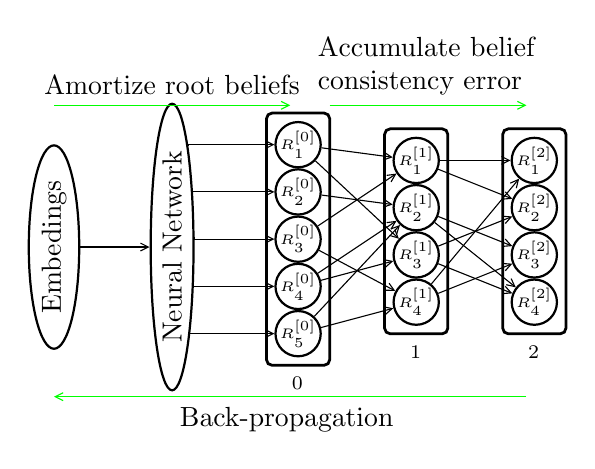
\begin{tikzpicture}
      \tikzstyle{enode} = [thick, draw=black, ellipse, inner sep = 2pt,  align=center]
      \tikzstyle{cnode} = [thick, draw=black, circle, inner sep = 0.0pt,  align=center]
      \tikzstyle{nnode} = [thick, rectangle, rounded corners = 0pt,draw,inner sep = 2pt]
      \begin{scope}[xshift=-1cm, yshift=-1.3cm, scale=0.6]
        \node[enode, rotate=90] (em) at (-2.5,0) {Embedings};
        \node[enode, rotate=90] (nn) {Neural Network};
      \end{scope}
      
      % level0 regions
      \begin{scope}[scale=0.6]
        \node[cnode] (r01) at (1, 0) {\tiny$R_1^{[0]}$};
        \node[cnode] (r02) at (1, -1) {\tiny$R_2^{[0]}$};
        \node[cnode] (r03) at (1, -2) {\tiny$R_3^{[0]}$};
        \node[cnode] (r04) at (1, -3) {\tiny$R_4^{[0]}$};
        \node[cnode] (r05) at (1, -4) {\tiny$R_5^{[0]}$};
        \node[label=below:$\Rr_0$, draw,rounded corners = 2pt, inner sep=1mm, fit=(r01) (r05)] {};
      \end{scope}

      \draw[->] (nn.351.9) |- (r01);
      \draw[->] (nn.340) |- (r02);
      \draw[->] (nn.295) |- (r03);
      \draw[->] (nn.210) |- (r04);
      \draw[->] (nn.191) |- (r05);

      \draw[->] (em) -- (nn);


      % level 1 regions
      \begin{scope}[xshift=1.5cm, yshift=-0.2cm, scale=0.6]
        \node[cnode] (r11) at (1, 0) {\tiny$R_1^{[1]}$};
        \node[cnode] (r12) at (1, -1) {\tiny$R_2^{[1]}$};
        \node[cnode] (r13) at (1, -2) {\tiny$R_3^{[1]}$};
        \node[cnode] (r14) at (1, -3) {\tiny$R_4^{[1]}$};
        \node[label=below:$\Rr_1$, draw, rounded corners = 2pt, inner sep=1mm, fit=(r11) (r14)] {};
      \end{scope}

      
      
      % level 1 regions
      \begin{scope}[xshift=3cm, yshift=-0.2cm, scale=0.6]
        \node[cnode] (r21) at (1, 0) {\tiny$R_1^{[2]}$};
        \node[cnode] (r22) at (1, -1) {\tiny$R_2^{[2]}$};
        \node[cnode] (r23) at (1, -2) {\tiny$R_3^{[2]}$};
        \node[cnode] (r24) at (1, -3) {\tiny$R_4^{[2]}$};
        \node[label=below:$\Rr_2$, draw, rounded corners = 2pt, inner sep=1mm, fit=(r21) (r24)] {};
      \end{scope}

      \draw[->] (r01) -- (r11);
      \draw[->] (r03) -- (r11);

      \draw[->] (r02) -- (r12);
      \draw[->] (r04) -- (r12);
      \draw[->] (r05) -- (r12);

      \draw[->] (r01) -- (r13);
      \draw[->] (r04) -- (r13);

      \draw[->] (r03) -- (r14);
      \draw[->] (r05) -- (r14);


      \draw[->] (r11) -- (r21);
      \draw[->] (r14) -- (r21);

      \draw[->] (r11) -- (r22);
      \draw[->] (r13) -- (r22);

      \draw[->] (r12) -- (r23);
      \draw[->] (r14) -- (r23);

      \draw[->] (r12) -- (r24);
      \draw[->] (r13) -- (r24);

      \draw[green, ->] (-2.5,0.5) --node[black,midway,above]{Amortize root beliefs} (0.5,0.5);
      \draw[green, ->] (1,0.5) --node[text width=2.8cm, black,midway,above]{Accumulate belief consistency error} (3.5,0.5);
      \draw[green, ->] (3.5,-3.2) --node[text width=2.8cm, black,midway,below]{Back-propagation} (-2.5,-3.2);
      
      
    \end{tikzpicture}
  \end{columns}
  
\end{frame}

\begin{frame}[label=current]{RENN}
  \onslide<1->{
    Non-root belief: \\
    \begin{center}
    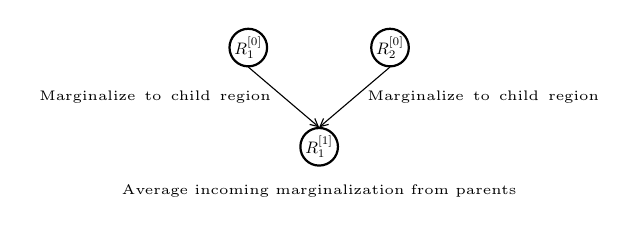
\begin{tikzpicture}
        \begin{scope}[yshift=-2cm, scale=0.6, every node/.append style={transform shape}]
          \tikzstyle{cnode} = [thick, draw=black, circle, inner sep = 1pt,  align=center]
              \tikzstyle{rnode} = [thick, circle, rounded corners = 2pt,minimum size = 0.0cm,draw,inner sep = 0.5pt]
          \node[rnode] (r01) at (0,0) {$R_1^{[0]}$};
          \node[rnode] (r02) at (3,0) {$R_2^{[0]}$};
          \node[rnode] (r11) at (1.5, -2.1) {$R_1^{[1]}$};
        \end{scope}

        \draw[->] (r01.south) -- node[align=center, text width=3cm, black,midway,left]{\tiny Marginalize to child region} (r11.north);
        \draw[->] (r02.south) -- node[align=center, text width=3cm, black,midway,right]{\tiny Marginalize to child region}(r11.north);
        \node[below=0.1cm of r11] {\tiny Average incoming marginalization from parents};
      \end{tikzpicture}
    \end{center}
    
    Objective of RENN:\\
    \begin{equation*}
      \min_{\text{\begin{tabular}{c}parameter \\of NN\end{tabular}}} \mathrm{\underbrace{\textbf{region-based free energy} (F_R)}_{\text{Assumulated average of all regions}}} + \underbrace{\mathrm{\textbf{panelty on belief consistency} }}_{\text{Recursively computed via levels of region graph}}
    \end{equation*}
  }
  \\
  \onslide<2->{
    RENN Inference:
    \begin{center}
    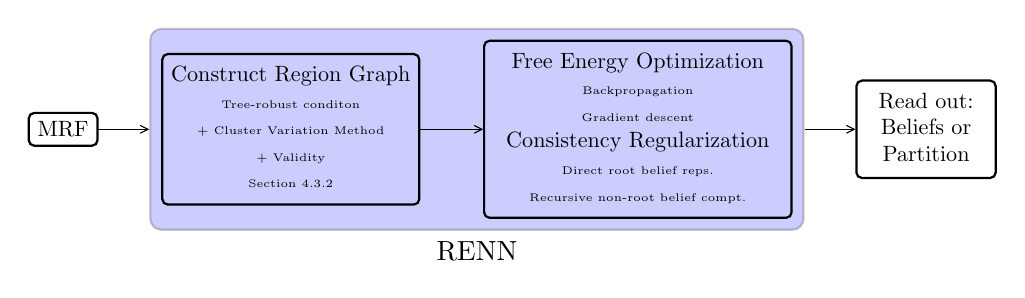
\begin{tikzpicture}
      %%%%%%%%%%%%%%%%%%%%%%%%%%%%%%%%%%%%%%%%%%%%%%%%%% 
      %% use of RENN
      %%%%%%%%%%%%%%%%%%%%%%%%%%%%%%%%%%%%%%%%%%%%%%%%%% 
      \tikzstyle{cnode} = [thick, draw=blue, rounded corners = 4pt, rectangle, inner sep = 4pt,  align=center]
      \tikzstyle{nnode} = [thick, rectangle, rounded corners = 0pt,draw,inner sep = 2pt]
      \tikzstyle{rnode} = [thick, rectangle, rounded corners = 2pt,minimum size = 0.0cm,draw,inner sep = 4pt]
      \begin{scope}[scale=0.8, every node/.append style={transform shape} ]
        \node[rnode] (r01) at (-1,0) {MRF};
        \node[rnode, right=of r01] (r02) {\begin{tabular}[x]{@{}c@{}} Construct Region Graph\\ {\tiny Tree-robust conditon} \\ {\tiny $+$ Cluster Variation Method} \\ {\tiny $+$ Validity} \\ {\tiny Section 4.3.2}\end{tabular}};
        \node[rnode, right=of r02] (r03) {\begin{tabular}{c}Free Energy Optimization\\ {\tiny Backpropagation}\\ {\tiny Gradient descent} \\ Consistency Regularization\\ {\tiny Direct root belief reps.} \\ {\tiny Recursive non-root belief compt.}\end{tabular}};
        \node[rnode, right=of r03] (r04) {\begin{tabular}{c}Read out: \\Beliefs or \\Partition\end{tabular}};
      \end{scope}
      \begin{scope}[on background layer]
        \node[cnode, fit=(r02)(r03), label=below:{RENN}, draw=black, fill=blue, opacity=0.2] (renn) {};
      \end{scope}
      \draw[->] (r01) -- (renn);
      \draw[->] (renn) -- (r04);
      \draw[->] (r02) -- (r03);
    \end{tikzpicture}
    \end{center}
  }
  % \onslide<2->{
  %   Learning alternatives of MRFs
  %   \begin{columns}
  %     \column{0.5\textwidth}
  %     learn with customized optm.
  %     \begin{align*}
  %       \pd{\log{p}(\bm{x};\bm{\theta})}{\bm{\theta}_a} = &\pd{\log{{\phi_a}(\bm{x}_a; \bm{\theta}_a)}}{\bm{\theta}_a} \\
  %                                                         &- \underbrace{\EE_{p(\bm{x}_a; \bm{\theta})}\left[ \pd{\log{{\phi_a}(\bm{x}_a; \bm{\theta}_a)}}{\bm{\theta}_a} \right]}_{\text{est. by beliefs}}.
  %     \end{align*}
  %     \column{0.5\textwidth}
  %     learn with auto-grads
  %     \begin{align*}
  %       \max_{\bm{\theta}} \log{p(\bm{x}; \bm{\theta})} =  &\max_{\bm{\theta}}\sum_{a}\log{ \psi_a(\bm{x}_a; \bm{\theta}_a) } \\
  %                                                          &\underbrace{ -\log{Z(\bm{\theta})}}_{\text{\begin{tabular}{c}ets. by the\\ Helmholtz free energy\\ $-\log{Z(\bm{\theta})} \simeq F_R$ \end{tabular}}}.
  %     \end{align*}
  %   \end{columns}
  % }
\end{frame}
\begin{frame}[label=current]{Insights of RENN}
  \begin{block}{Generalization}
    Bethe free energy can be recovered from region-based free energy:
    \begin{itemize}[label=\textbullet]
    \item two-level region graph representation
    \item constraint that each region can contain at most one factor node
    \end{itemize}
    {\tiny Section 4.2.1}
  \end{block}
  \begin{block}{Attributes of RENN}
    \begin{itemize}[label=\textbullet]
    \item RENN requires neither sampling technique nor training data (ground-truth marginal probabilities) in performing inference tasks;
    \item RENN does gradient descent w.r.t. its neural network parameter instead of iterative message-passing, and returns approximation of marginal probabilities and partition estimation in one-shot
    \item No message propagation, thus no need of message scheduling
    \item Competitive performance and efficiency
    \end{itemize}
  \end{block}
\end{frame}

\begin{frame}[label=current]{Some Numerical Comparisons}
  
  Ising model: $p(\bm{x}; \bm{\theta}) = \frac{1}{Z(\bm{\theta})}\exp{(\sum_{(i,j)\in \Ee_F} J_{ij} x_i x_j + \sum_{i\in \Vv}h_i x_i)}$, $\bm{x} \in \{-1, 1\}^{N}$,
  \begin{itemize}[label=$\bullet$]
  \item $J_{ij}$ is the pairwise log-potential between node $i$ and $j$, $J_{ij}\sim \Nn(0,1)$
  \item  $h_i$ is the node log-potential for node $i$, $h_i \sim \Nn(0, \gamma^{2})$
  \end{itemize}
  
  Inference on grid graph ($\gamma=0.1$). 
  \begin{adjustbox}{width=1\textwidth}
    \begin{tabular}{lcccccccc}
      \toprule
      Metric & $n$ & Mean Field & Loopy BP & Damped BP & GBP & Inference Net & RENN \\
      \midrule
      \multirow{4}{*}{\begin{tabular}[x]{@{}c@{}}$\ell_1$\\error \end{tabular} }
             &    25   &$0.271 \pm 0.051$ &  $0.086 \pm 0.078$ & $0.084 \pm 0.076$ & $0.057 \pm 0.024$ & $0.111 \pm 0.072$ & \textbf{0.049} $\pm$ 0.078 \\

             &    100   & $0.283 \pm 0.024$ &  $0.085 \pm 0.041$ & $0.062 \pm 0.024$ & $0.064 \pm 0.019$ & $0.074 \pm 0.034$ & \textbf{0.025} $\pm$ 0.011 \\

             &    225   & $0.284 \pm 0.019$ &  $0.100 \pm 0.025$ & $0.076 \pm 0.025$ & $0.073 \pm 0.013$ & $ 0.073 \pm 0.012$ & \textbf{0.046} $\pm$ 0.011 \\

             &    400   & $0.279 \pm 0.014$ &  $0.110 \pm 0.016$ & $0.090 \pm 0.016$ & $0.079 \pm 0.009$ & $ 0.083 \pm 0.009$ & \textbf{0.061} $\pm$ 0.009 \\

      \midrule
      \multirow{4}{*}{\begin{tabular}[x]{@{}c@{}}Corre-\\lation\\ $\rho$ \end{tabular}}
             &   25    & 0.633 $\pm$ 0.197  &  0.903 $\pm$ 0.114  &  0.905 $\pm$ 0.113  &  0.923 $\pm$ 0.045  &  0.866$\pm$ 0.117 &  \textbf{0.951} $\pm$ 0.112 \\

             &   100   & 0.582 $\pm$ 0.112  &  0.827 $\pm$ 0.134  &  0.902 $\pm$ 0.059  &  0.899 $\pm$ 0.043  &  0.903$\pm$ 0.049 &   \textbf{0.983} $\pm$ 0.012 \\

             &   225   & 0.580 $\pm$ 0.080  &  0.801 $\pm$ 0.078  &  0.863 $\pm$ 0.088  &  0.869 $\pm$ 0.037  & 0.873 $\pm$ 0.037 &  \textbf{0.949} $\pm$ 0.022 \\

             &   400   & 0.596 $\pm$ 0.054  &  0.779 $\pm$ 0.059  &  0.822 $\pm$ 0.047  &  0.852 $\pm$ 0.024  & 0.841 $\pm$ 0.028 &  \textbf{0.912} $\pm$ 0.025 \\

      \midrule
      \multirow{4}{*}{\begin{tabular}[x]{@{}c@{}}$\log{Z}$ \\error\end{tabular}}
             &   25    & 2.512 $\pm$ 1.060  &  0.549 $\pm$ 0.373  &  0.557 $\pm$ 0.369  &  \textbf{0.169} $\pm$ 0.142  &  0.762 $\pm$ 0.439  &  0.240 $\pm$ 0.140 \\

             &  100    & 13.09 $\pm$ 2.156  &  1.650 $\pm$ 1.414  &  1.457 $\pm$  1.365 &  \textbf{0.524} $\pm$ 0.313  &  2.836 $\pm$ 2.158  & 1.899 $\pm$ 0.495 \\

             &  225    & 29.93 $\pm$ 4.679  &  3.348 $\pm$ 1.954  &  3.423 $\pm$ 2.157  &  \textbf{1.008} $\pm$ 0.653  &  3.249 $\pm$ 2.058  & 4.344 $\pm$ 0.813  \\

             &  400    & 51.81 $\pm$ 4.706  &  5.738 $\pm$ 2.107  &  5.873$\pm$ 2.211   &  \textbf{1.750} $\pm$ 0.869  &  3.953 $\pm$ 2.558  & 7.598 $\pm$ 1.146 \\

      \bottomrule
    \end{tabular}
  \end{adjustbox}
  \begin{itemize}[label=$\bullet$]
  \item $\ell_1$ error of beliefs v.s. true
  \item correlation $\rho$ between true and approximate marginals,
  \item $\log{Z}$ error, true v.s. free energy approximation.
  \end{itemize}
  
\end{frame}
\begin{frame}[label=current]
  {Some Numerical Comparisons}
  {Richer Comparisons}
  Inference on grid and complete graphs.
  \begin{table}
    \vskip -0.1in
    \begin{adjustbox}{width=1\textwidth}
      \begin{small}
        \begin{tabular}{cl c ccccccc}
          \toprule
          {}&{}& Metric & {} & Mean Field & Loopy BP & Damped BP & GBP & Inference Net & RENN \\
          \midrule
          \multirow{4}{*}{\rotatebox[origin=c]{90}{\begin{tabular}{c}High Temp\\-erature\end{tabular}}}%  &
            &\multirow{4}{*}{\rotatebox[origin=c]{0}{\begin{tabular} [x]{@{}c@{}} Complete graph \\ N=16 \\$J_{ij}\sim \Nn(0,1)$ \\ $h_i \sim \Nn(0, \gamma^{2})$ \end{tabular}}} &
                                                                                                                                                                                    \multirow{2}{*}{\begin{tabular}[x]{@{}c@{}}$\ell_1$-\\error\end{tabular}}
            & $\gamma=1$   &  0.273 $\pm$ 0.086  &  0.239 $\pm$ 0.059  &  0.239 $\pm$ 0.059  &  0.260 $\pm$ 0.086  &  0.249 $\pm$ 0.067  &  \textbf{0.181} $\pm$ 0.092  \\
            & &       &  $\gamma=4$    &  0.197 $\pm$0.049   &  0.181 $\pm$ 0.035  &  0.180 $\pm$ 0.034  &  0.210 $\pm$ 0.070  &  0.174 $\pm$ 0.030  &  \textbf{0.125} $\pm$ 0.050  \\
          \cmidrule{3-10}
            &&\multirow{2}{*}{\begin{tabular}[x]{@{}c@{}}$\log{Z}$ \\error\end{tabular}}
            &  $\gamma=1$    &  20.66 $\pm$ 5.451  &  178.7 $\pm$ 22.18  &  178.9 $\pm$ 21.88  &  153.3 $\pm$ 25.29  &  213.6 $\pm$ 12.75  &  \textbf{14.41} $\pm$ 4.135  \\
            &&      &  $\gamma=4$    &  \textbf{10.74} $\pm$ 7.385  &  565.7 $\pm$ 73.33  &  566.1 $\pm$ 73.13  &  106.0 $\pm$ 54.43  &  588.3 $\pm$ 62.58  &  14.72 $\pm$ 4.155  \\
          
          
          \bottomrule
          {\multirow{4}{*}{\rotatebox[origin=c]{90}{\begin{tabular}{c}Low Temp\\-erature\end{tabular}}}}&\multirow{4}{*}{\rotatebox[origin=c]{0}{\begin{tabular} [x]{@{}c@{}} Grid graph \\ N=100\\ $J_{ij}\sim \Uu(-u,u)$ \\ $h_i \sim \Uu(-1, 1)$ \end{tabular}}}
            &\multirow{2}{*}{\begin{tabular}[x]{@{}c@{}}$\ell_1$\\error \end{tabular} }
            &    5   & $0.257 \pm 0.065$ &  $0.115 \pm 0.071$ & $0.120 \pm 0.073$ & $0.250 \pm 0.024$ & $ 0.164 \pm 0.036$ & \textbf{0.100} $\pm$ 0.046 \\

            &&&    15  & $0.328 \pm 0.068$ &  $0.228 \pm 0.088$ & $0.267 \pm 0.147$ & $0.303 \pm 0.026$ & $ 0.279 \pm 0.024$ & \textbf{0.207} $\pm$ 0.054 \\
          \cmidrule{3-10}
            & &\multirow{2}{*}{\begin{tabular}[x]{@{}c@{}}$\log{Z}$ \\error\end{tabular}}
            &  5     & 42.65 $\pm$ 17.86  &  7.346 $\pm$ 7.744  &  \textbf{5.444} $\pm$ 4.811  &  {8.369} $\pm$ 7.401  &  65.60 $\pm$ 8.786  & 11.34 $\pm$ 4.724 \\
            &&      &  15    & 164.9 $\pm$ 56.07  &  58.40 $\pm$ 41.36  &  101.9 $\pm$ 54.31  &  \textbf{23.10} $\pm$ 15.06  &  224.3 $\pm$ 25.52  & 78.85 $\pm$ 15.08 \\
          \bottomrule
        \end{tabular}
      \end{small}
    \end{adjustbox}
    \vskip -0.1in
  \end{table}
  {Average consumed time per inference instance (unit: second)}
  \begin{table}
    
    \vskip -0.1in
    \centering
    \begin{adjustbox}{width=0.98\textwidth}
      \begin{tabular}{lcccccc}
        \toprule
        {} &  Mean Field & Loopy BP & Damped BP & GBP & Inference Net & RENN \\
        \toprule
        Grid $\Gg$, $N=400$, $J_{ij}\sim \Nn(0,1), h_i\sim\Nn(0,0.1^2)$ & 9.897 & 425.0 & 328.3 & 286.3 & 74.41 & 101.0 \\
        Complete $\Gg$, $N=16$, $J_{ij}\sim \Nn(0,1), h_i\sim\Nn(0,1)$ & 0.457 & 0.777 & 1.285 & 14.29 &  12.45  & 16.16\\
        Grid $\Gg$, $N=100$, $J_{ij}\sim \Uu(-15,15), h_i\sim\Uu(-1,1)$ & 2.314 & 253.3 & 229.3 & 53.72 & 103.4 & 79.38 \\
        Complete $\Gg$, $N=9$, $J_{ij}\sim \Uu(-15,15), h_i\sim\Uu(-1,1)$ & 0.502 & 15.86 & 18.23 & 3.213 & 17.21 & 7.857 \\
        \bottomrule
      \end{tabular}
    \end{adjustbox}
  \end{table}
\end{frame}
%%% Local Variables:
%%% mode: latex
%%% TeX-master: "../ppgm_slide"
%%% End:



%%%%%%%%%%%%%%%%%%%%%%%%%%%%%%%%%%%%%%%%%%%%%%%%%%%%%% 
% ------------------------------------------------
% section learning
%%%%%%%%%%%%%%%%%%%%%%%%%%%%%%%%%%%%%%%%%%%%%%%%%%%%%% 
\section{Learning}
\subsection{Bidirectional Impact}

{ \setbeamercolor{background canvas}{bg=hl_bg}
  \setbeamercolor{normal text}{fg=hl_fg}
  \setbeamercolor{frametitle}{fg=hl_fg}
  \begin{frame}
    \usebeamercolor[fg]{normal text}
    \begin{center}
      {
        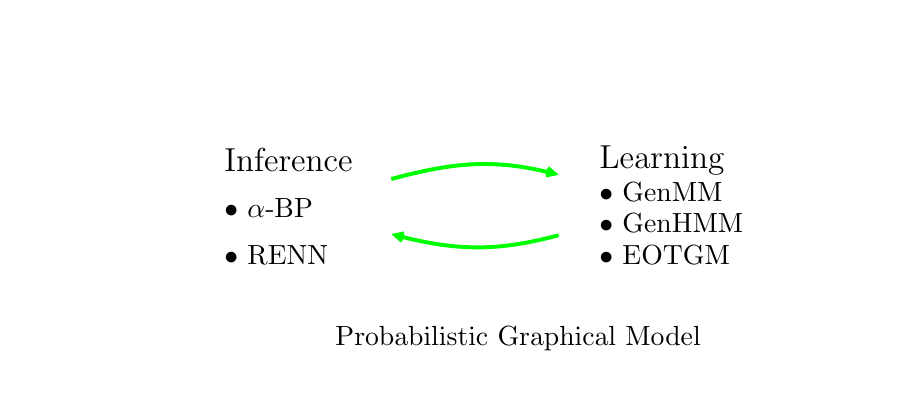
\begin{tikzpicture}
          \tikzstyle{cnode} = [thick, draw=white, ellipse, inner sep = 2pt,  align=center]
          \tikzstyle{fnode} = [thick, draw=white, ellipse, inner sep = 10pt,  align=center]
          \tikzstyle{rnode} = [thick, rectangle, inner sep = 1.5pt,  align=left]
          \node[rnode] (inf) at (-2, 0) {\large Inference};
          \node[rnode, below = 0.6cm of inf.west, anchor=west] (abp) {$\bullet$ {$\alpha$-BP}};
          \node[rnode, below = 1.2cm of inf.west, anchor=west] (renn) {$\bullet$ RENN};
          \node[cnode, fit=(abp)(inf)(renn)] (infn) {};
          
          \node[rnode, right = 3 of inf] (lern) {\large Learning};
          \node[rnode, below = 0.4 of lern.west, anchor=west] (genmm) {$\bullet$ GenMM};
          \node[rnode, below = 0.8 of lern.west, anchor=west] (genhmm) {{$\bullet$} GenHMM};
          \node[rnode, below = 1.2 of lern.west, anchor=west] (lfree) {{$\bullet$} EOTGM};
          \node[cnode, fit=(lern)(genmm)(genhmm)(lfree)] (learn) {};

          \node[fnode, fit=(infn)(lern)] (box) {};

          
          \node[below right = 0.5 and -0.5 of infn] {{Probabilistic} Graphical Model};
          \draw[->,line width=0.5mm, green] (infn) to[out=15, in=165] (learn);
          \draw[->,line width=0.5mm, green] (learn) to[out=195, in=-15] (infn);
        \end{tikzpicture}
      }
    \end{center}
    
  \end{frame}
}
\begin{frame}{Two Direction Impact}
  Why impact in two direction?
  \begin{itemize}[label=$\bullet$]
    \onslide<1->{
    \item Learning to Inference:\\
      \begin{figure}[!t]
        \centering
        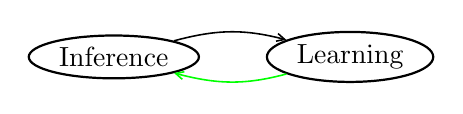
\begin{tikzpicture}
          \tikzstyle{cnode} = [thick, draw=black, ellipse, inner sep = 2pt,  align=center]
          \tikzstyle{fnode} = [thick, draw=black, ellipse, inner sep = 10pt,  align=center]
          
          \node[cnode] (infn) at (0,0) {Inference};
          \node[cnode] (lern) at (3,0) {Learning};
          
          % \node[fnode, fit=(infn)(lern)] (box) {};
          % \node[] at (1.4, -0.6) {Probabilistic Graphical Model};
          \draw[->,line width=0.2mm] (infn) to[out=15, in=165] (lern);
          \draw[green, ->,line width=0.2mm] (lern) to[out=195, in=-15] (infn);
        \end{tikzpicture}
      \end{figure}
      Stuff we have been taken as default, a given $p(\bm{x};\bm{\theta})$
      \begin{itemize}[label=$\bullet$]
      \item built by expert knowledge, or
      \item built by extracting information from evidence (empirical data).
      \end{itemize}
    }
    \onslide<2->{
    \item Inference to Learning:\\
      \begin{figure}[!t]
        \centering
        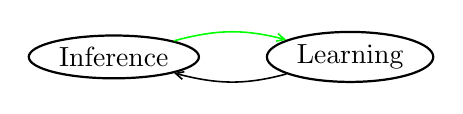
\begin{tikzpicture}
          \tikzstyle{cnode} = [thick, draw=black, ellipse, inner sep = 2pt,  align=center]
          \tikzstyle{fnode} = [thick, draw=black, ellipse, inner sep = 10pt,  align=center]
          
          \node[cnode] (infn) at (0,0) {Inference};
          \node[cnode] (lern) at (3,0) {Learning};
          
          % \node[fnode, fit=(infn)(lern)] (box) {};
          % \node[] at (1.4, -0.6) {Probabilistic Graphical Model};
          \draw[green, ->,line width=0.2mm] (infn) to[out=15, in=165] (lern);
          \draw[->,line width=0.2mm] (lern) to[out=195, in=-15] (infn);
        \end{tikzpicture}
      \end{figure}
      Model learning: an error trial process that compares inferred 'fact' and actual fact (evidence).\\
      Model learning usually needs inference as a subroutine, which sometimes are replaced by sampling in particle based methods.
    }
  \end{itemize}
  
  
\end{frame}
\begin{frame}[label=current]{\large Inference Routine in Learning}
  
  What is $\bm{\theta}$ in $p(\bm{x}; \bm{\theta}) = \frac{1}{Z(\bm{\theta})} \prod_{a} \psi_a(\bm{x}_a; \bm{\theta}_a)$? \\
  A direct view:
  \begin{align*}
    \max_{\bm{\theta}} \log{p(\bm{x}; \bm{\theta})} =  \max_{\bm{\theta}}\sum_{a}\log{ \psi_a(\bm{x}_a; \bm{\theta}_a) } \underbrace{- \log{Z(\bm{\theta})}}_{\text{Helmholtz free energy, can be est. by $F$}},
  \end{align*}
  An alternative view:
  \begin{align*}
    \pd{\log{p}(\bm{x};\bm{\theta})}{\bm{\theta}_a} = \pd{\log{{\phi_a}(\bm{x}_a; \bm{\theta}_a)}}{\bm{\theta}_a} - \underbrace{\EE_{p(\bm{x}_a; \bm{\theta})}\left[ \pd{\log{{\phi_a}(\bm{x}_a; \bm{\theta}_a)}}{\bm{\theta}_a} \right]}_{\text{can be est. by beliefs}}.
  \end{align*}

  Remark:
  \begin{itemize}[label={$\bullet$}]
  \item This essentially requires estimation of Helmholtz free energy or marginal probabilities.
  \item Stationary points translate into moment matching.
  \end{itemize}
  \only<2->{
  \begin{textblock}{5}(3,10)
    \begin{tikzpicture}[auto,rotate=-5,transform shape]
      \tikzstyle{cnode} = [thick, draw=black, ellipse, inner sep = 2pt,  align=center]
      \tikzstyle{fnode} = [thick, draw=black, ellipse, inner sep = 10pt,  align=center]
          
      \node[cnode] (infn) at (0,0) {Inference};
      \node[cnode] (lern) at (3,0) {Learning};
      
      \draw[->,line width=0.2mm] (infn) to[out=15, in=165] (lern);
      \draw[->,line width=0.2mm] (lern) to[out=195, in=-15] (infn);

      \node[text width=7cm, align=left, below =of infn.west, anchor=west] (uncouple)
      {\begin{minipage}{1\textwidth}
          \begin{itemize}[label=\textbullet]
          \item Two modules are not necessarily coupled
          \item Each module may be replaced by another algorithm while the other one remains.
          \end{itemize}
        \end{minipage}
      };
      \begin{scope}[on background layer]
        \node [rounded corners = 4pt, rectangle, inner sep = 4pt,  align=center, fit=(uncouple)(infn)(lern), label=below:{}, fill=blue!30] () {};
      \end{scope}
    \end{tikzpicture}
  \end{textblock}
}
\end{frame}

% \begin{frame}[label=current]{\large Inference Routine in Learning}
%   \begin{tikzpicture}
%     \node[black] (grad) at (0,0) {
%     \begin{minipage}{1\linewidth}
%       What is $\bm{\theta}$ in $p(\bm{x}; \bm{\theta}) = \frac{1}{Z(\bm{\theta})} \prod_{a} \psi_a(\bm{x}_a; \bm{\theta}_a)$? \\
%       A direct view:
%       \begin{align*}
          %           \max_{\bm{\theta}} \log{p(\bm{x}; \bm{\theta})} =  \max_{\bm{\theta}}\sum_{a}\log{ \psi_a(\bm{x}_a; \bm{\theta}_a) } \underbrace{- \log{Z(\bm{\theta})}}_{\text{Helmholtz free energy, can be est. by $F$}},
          %         \end{align*}
          %           An alternative view:
          %           \begin{align*}
          %           \pd{\log{p}(\bm{x};\bm{\theta})}{\bm{\theta}_a} = \pd{\log{{\phi_a}(\bm{x}_a; \bm{\theta}_a)}}{\bm{\theta}_a} - \underbrace{\EE_{p(\bm{x}_a; \bm{\theta})}\left[ \pd{\log{{\phi_a}(\bm{x}_a; \bm{\theta}_a)}}{\bm{\theta}_a} \right]}_{\text{can be est. by beliefs}}.
          %         \end{align*}

          %           Remark:
          %           \begin{itemize}[label={$\bullet$}]
          %           \item This essentially requires estimation of Helmholtz free energy or marginal probabilities.
          %           \item Stationary points translate into moment matching.
          %           \end{itemize}
          %           \end{minipage}
          %           };
          %           \pause {
          %           \begin{scope}[local bounding box=uncouple]
          %           \tikzstyle{cnode} = [thick, draw=black, ellipse, inner sep = 2pt,  align=center]
          %           \tikzstyle{fnode} = [thick, draw=black, ellipse, inner sep = 10pt,  align=center]

          %           \node[cnode] (infn) at (0,0) {Inference};
          %           \node[cnode] (lern) at (3,0) {Learning};
          %           \node[black, above=of infn.north] (txt1) {at The two modules are not necessarily coupled};
          %         %           \node[fnode, fit=(infn)(lern)] (box) {};
          %         %           \node[] at (1.4, -0.6) {Probabilistic Graphical Model};
          %           \draw[->,line width=0.2mm] (infn) to[out=15, in=165] (lern);
          %           \draw[->,line width=0.2mm] (lern) to[out=195, in=-15] (infn);
          %           \node[black,fill=white, below=of infn.south] (txt2) {Each module may be replaced by another algorithm while the other one remains.};
          %           \begin{scope}[on background layer]
          %           \node[rectangle, inner sep = 10pt,  align=center, fit=(txt1)(txt2)(infn)(learn), fill=white] {};
          %           \end{scope}

          %           \end{scope}

          %           }  
          %           \end{tikzpicture}
          %           \end{frame}




\begin{frame}
  {Learning MRFs}
  {What is $\bm{\theta}$ in $p(\bm{x};\bm{\theta})$?}
  \vskip 0.5cm
  Table of negative log-likelihood of learned MRFs \\
  \begin{table}
    \begin{adjustbox}{width=0.9\textwidth}
      \begin{tabular}{lcccccccc}
        % std=1.0
        \toprule
        N & True & Exact & Mean Field & Loopy BP & Damped BP & GBP & Inference Net & RENN \\
        \toprule
        \multicolumn{9}{c}{Grid Graph}\\
        \midrule
        25  &  9.000  &  9.004  &  9.811  &  {9.139}  &  9.196  &  10.56  &  9.252  &  \textbf{9.048}  \\
        100 &  19.34  &  19.38  &  23.48  &  {19.92}  &  20.02  &  28.61  &  20. 29  &  \textbf{19.76} \\
        225 &  63.90  &  63.97  &  69.01  &  66.44    &  66.25  &  92.62  &  68.15  &  \textbf{64.79}  \\
        \toprule
        % std=1.0
        \multicolumn{9}{c}{Complete Graph}\\
        \midrule
        9  &  3.276  &  3.286  &  9.558  &  5.201  &  5.880  &  10.06  &  5.262  & \textbf{3.414}  \\
        16  &  4.883  &  4.934  &  28.74  &  13.64  &  18.95  &  24.45  &  13.77  &  \textbf{5.178}  \\

        \bottomrule
      \end{tabular}
    \end{adjustbox}
  \end{table}
  \vskip 0.5cm
  {Average consumed time per epoch (unit: second) for two MRF learning cases.}
  \begin{table}
    \centering
    \begin{adjustbox}{width=0.9\textwidth}
      \begin{tabular}{lcccccc}
        \toprule
        {} &  Mean Field & Loopy BP & Damped BP & GBP & Inference Net & RENN \\
        \toprule
        Grid $\Gg$,\! $N\!=\!225\!\!$ & 40.09 & 335.1 & 525.1 & 12.37 & 19.49 & 16.03 \\
        Complete\! $\Gg$,\! $N=\!16\!\!$ & 2.499 & 12.40 & 5.431 & 1.387 & 0.882 & 2.262 \\
        \bottomrule
      \end{tabular}
    \end{adjustbox}
  \end{table}

\end{frame}

%%% Local Variables:
%%% mode: latex
%%% TeX-master: "../ppgm_slide"
%%% End:


\subsection{Flow-EM}

{ \setbeamercolor{background canvas}{bg=hl_bg}
  \setbeamercolor{normal text}{fg=hl_fg}
  \setbeamercolor{frametitle}{fg=hl_fg}
  \begin{frame}
    \usebeamercolor[fg]{normal text}
    \begin{center}
      {
        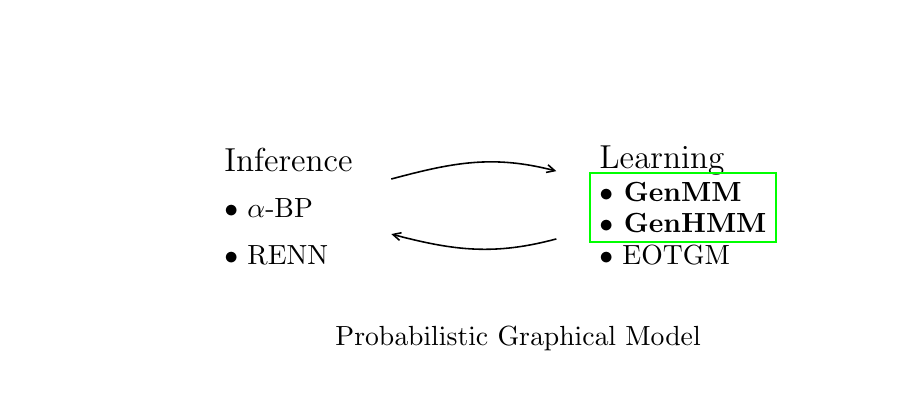
\begin{tikzpicture}
          \tikzstyle{cnode} = [thick, draw=white, ellipse, inner sep = 2pt,  align=center]
          \tikzstyle{fnode} = [thick, draw=white, ellipse, inner sep = 10pt,  align=center]
          \tikzstyle{rnode} = [thick, rectangle, inner sep = 1.5pt,  align=left]
          \node[rnode] (inf) at (-2, 0) {\large Inference};
          \node[rnode, below = 0.6cm of inf.west, anchor=west] (abp) {$\bullet$ {$\alpha$-BP}};
          \node[rnode, below = 1.2cm of inf.west, anchor=west] (renn) {$\bullet$ RENN};
          \node[cnode, fit=(abp)(inf)(renn)] (infn) {};
          
          \node[rnode, right = 3 of inf] (lern) {\large Learning};
          \node[rnode, below = 0.4 of lern.west, anchor=west] (genmm) {\textbf{$\bullet$ GenMM}};
          \node[rnode, below = 0.8 of lern.west, anchor=west] (genhmm) {\textbf{{$\bullet$} GenHMM}};
          \node[rnode, below = 1.2 of lern.west, anchor=west] (lfree) {{$\bullet$} EOTGM};
          \node[cnode, fit=(lern)(genmm)(genhmm)(lfree)] (learn) {};
          \node[rnode, draw=green, fit=(genmm)(genhmm)] () {};

          \node[fnode, fit=(infn)(lern)] (box) {};

          
          \node[below right = 0.5 and -0.5 of infn] {{Probabilistic} Graphical Model};
          \draw[->,line width=0.2mm] (infn) to[out=15, in=165] (learn);
          \draw[->,line width=0.2mm] (learn) to[out=195, in=-15] (infn);
        \end{tikzpicture}
      }
    \end{center}
    
  \end{frame}
}
\begin{frame}[label=current]
  {Incomplete Observation}
  Partial observation: $\bm{x} = [  \underbrace{\bm{x}_U}_{Unobserved}, \underbrace{\bm{x}_O}_{Observed}]$
  \begin{equation*}
    l(\bm{x}_O; \bm{\theta}) = \log{\sum_{\bm{x}_U}p(\bm{x}_U, \bm{x}_O; \bm{\theta})} = \log{\underbrace{Z(\bm{x}_O;\bm{\theta})}_{\sum_{\bm{x}_U}\tilde{p}(\bm{x}; \bm{\theta})}} - \log{Z(\bm{\theta})},
  \end{equation*}

  {Connect Free Energy to Evidence Lower Bounder}:
  \begin{columns}
    \column{0.6\textwidth}
    \begin{align*}
      l(\bm{x}_O; \bm{\theta}) &\geq - \underbrace{F_v(q(\bm{x}_U|\bm{x}_O))}_{Variational Free Energy} - \log{Z(\bm{\theta})} \nonumber \\
                               & = \EE_{q(\bm{x}_U|\bm{x}_O)}\left[ \log{\frac{{p}(\bm{x}_U, \bm{x}_O; \bm{\theta})}{q(\bm{x}_U|\bm{x}_O)}} \right] \nonumber \\
                               & = \underbrace{\EE_{q(\bm{x}_U|\bm{x}_O)}\left[ \log{{p}(\bm{x}_U, \bm{x}_O; \bm{\theta})} \right] + H({q(\bm{x}_U|\bm{x}_O)})}_{\text{Evidence Lower Bound $F(q, \bm{\theta})$}}
    \end{align*}
    
    \column{0.4\textwidth}
    Intuition of maximizing $F(q,\bm{\theta})$
    \begin{itemize}[label=\textbullet]
    \item Maximizing (incomplete) likelihood
    \item Minimizing free energy
    \end{itemize}

  \end{columns}
  This gives the EM as a coordinate ascent method:
  \begin{align*}
    \mathrm{E~step:}~~~ q^{(t+1)} &= \uargmax{q}{F(q, \bm{\theta}^{(t)})}, \\
    \mathrm{M~step:}~~~\bm{\theta}^{(t+1)} &= \uargmax{\bm{\theta}}{F(q^{(t+1)}, \bm{\theta})}.
  \end{align*}
\end{frame}


\begin{frame}[label=current]{Generator Mixed Model}
  {Equipping EM with Normalizing Flows}
  \begin{columns}
    \column{0.4\textwidth}
    \centering
    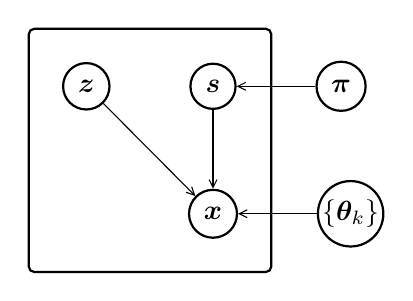
\begin{tikzpicture}
      \tikzstyle{enode} = [thick, draw=black, circle, align=center]
      \tikzstyle{cnode} = [thick, draw=black, circle, align=center, inner sep = 0.3pt]
      \tikzstyle{nnode} = [thick, rectangle, rounded corners = 2pt,minimum size = 0.8cm,draw,inner sep = 12pt]
      %%%%%%%%%%%%%%%%%%%%%%%%%%%%%%%%%%%%%%%% 
      %% directed graphical model
      %%%%%%%%%%%%%%%%%%%%%%%%%%%%%%%%%%%%%%%% 
      \begin{scope}[scale=1, every node/.append style={transform shape}]
        \node[enode] (x) at (0,0){$\bm{x}$};

\node[enode, above=of x] (s) {$\bm{s}$};
\node[enode, left=of s] (z) {$\bm{z}$};
\node[enode, right=of s] (pi) {$\bm{\pi}$};
\node[cnode, right=of x] (phi) {$\{ \bm{\theta}_k \}$};
\node[nnode, fit=(x)(z)(s)] (box) {};

\draw[->] (z) to (x);
\draw[->] (s) to (x);
\draw[->] (pi) to (s);
\draw[->] (phi) to (x);

%%% Local Variables:
%%% mode: latex
%%% TeX-master: "../ppgm_slide"
%%% End:

      \end{scope}

    \end{tikzpicture}
    
    \column{0.55\textwidth}
    
    \centering
    \begin{minipage}{\linewidth}
      
      \begin{itemize}[label=\textbullet]
      \item Ideal case: The underline true $p^{\ast}(\bm{x})$ is in hypothesis space $\Hh$, i.e. $p^{\ast}(\bm{x}) \in \Hh$.
      \item Out of reach: Test $p^{\ast}(\bm{x}) \stackrel{?}{\in} \Hh$
      \item A general desire:
        \begin{equation*}
          \Hh ~\mathrm{is~large}  \rightarrow \mathrm{condidate}~ p(\bm{x};\bm{\theta})~\mathrm{is~flexible}
        \end{equation*}
        
      \end{itemize}
      
      This brings up the finite \textbf{mixture} models.

      \begin{align*}\label{eq:FirstMixtureModel}
        p(\bm{x};\bm{\Theta})  = \textstyle\sum_{k=1}^K \pi_k  p_k(\bm{x}) = \textstyle \sum_{k=1}^K \pi_k  p(\underbrace{\bm{g}(\bm{z};\bm{\theta}_k)}_{\text{\begin{tabular}{c}Variable change \\via generator $\bm{g}$\end{tabular}}}).
      \end{align*}
      
    \end{minipage}
  \end{columns}
  
  \vskip -0.5cm
  What to expect from GenMM:
  \begin{itemize}[label=\textbullet]
  \item {Flexible and expressive model, enlarging hyperspace $\Hh$}
  \item {Tractable likelihood} 
  \item {Compatible with typical statistical models}
  \item Compatible with NN tools/frameworks
  \item {Scale to high-dimensional structured data}
  \item {Efficient in sampling (data generation)}
  \item {...}
  \end{itemize}

\end{frame}




\begin{frame}[label=current]{A High-level View of GenMM: finite mixture}
  \begin{tikzpicture}
    \tikzstyle{enode} = [thick, draw=black, circle, align=center]
    \tikzstyle{cnode} = [thick, draw=black, circle, align=center, inner sep = 0.3pt]
    \tikzstyle{nnode} = [thick, rectangle, rounded corners = 2pt,minimum size = 0.8cm,draw,inner sep = 22pt]
    %%%%%%%%%%%%%%%%%%%%%%%%%%%%%%%%%%%%%%%% 
    %% 1. directed graphical model
    %%%%%%%%%%%%%%%%%%%%%%%%%%%%%%%%%%%%%%%% 
    \begin{scope}[scale=0.6, every node/.append style={transform shape}, local bounding box=dgm, opacity=0.3]
      \node[enode] (x) at (0,0){$\bm{x}$};

\node[enode, above=of x] (s) {$\bm{s}$};
\node[enode, left=of s] (z) {$\bm{z}$};
\node[enode, right=of s] (pi) {$\bm{\pi}$};
\node[cnode, right=of x] (phi) {$\{ \bm{\theta}_k \}$};
\node[nnode, fit=(x)(z)(s)] (box) {};

\draw[->] (z) to (x);
\draw[->] (s) to (x);
\draw[->] (pi) to (s);
\draw[->] (phi) to (x);

%%% Local Variables:
%%% mode: latex
%%% TeX-master: "../ppgm_slide"
%%% End:

    \end{scope}
    
    %%%%%%%%%%%%%%%%%%%%%%%%%%%%%%%%%%%%%%%% 
    %% 2. illustration of GenMM
    %%%%%%%%%%%%%%%%%%%%%%%%%%%%%%%%%%%%%%%% 
    \begin{scope}[shift={($(dgm.east)+(3cm,0)$)}, local bounding box=illsGenMM]
      
% \tikzstyle{enode} = [thick, draw=blue, circle, inner sep = 3pt,
% align=center]
\tikzstyle{enode} = [thick, draw=black, ellipse, inner sep = 2pt,  align=center]
\tikzstyle{nnode} = [thick, rectangle, rounded corners = 2pt,minimum size = 0.8cm,draw,inner sep = 2pt]
\node[enode,label={below:{\tiny Shared latent source}}] (z) at (0,0) {$\bm{z}\sim p(\bm{z})$};
\node[enode, label={below:{\tiny Induced distribution}}] (x) at (5.5,0){$\bm{x}\sim p(\bm{x}; \bm{\Phi})$};
% \node at (5.2,-1) {$p(\bm{x};\bm{\Phi}) = \textstyle\sum_{k=1}^K \pi_k  p_k(\bm{x})$};
\node[nnode] (g1) at (2.6,1.8) {$\bm{g}_1$};
\node[nnode] (g2) at (2.6,0.5) {$\bm{g}_2$};
\node[nnode] (gk) at (2.6,-1.8) {$\bm{g}_K$};
\draw[dotted,line width=2pt] (2.6,-0.3) -- (2.6,-1.2);
\draw[->] (z) [in= 180, out =0] to (g1);
\draw[->] (z) [in= 180, out =0] to (g2);
\draw[->] (z) [in= 180, out =0] to (gk);
\filldraw[->] (3.7, 0.5)circle (2pt) -- node[above=0.2](switch){$\bm{s}\sim \bm{\pi}$} (x);
\node[above= 0.2 of switch.east] {\tiny \begin{tabular}{c}Categorical variable\\ as generator switch\end{tabular}};
% \draw[->] (3,-0.8) -- (3.5, -0.8);
\draw[->] (g1) -- (3.5,1.8);
\draw[->] (g2) -- (3.5, 0.5);
\draw[->] (gk) -- (3.5, -1.8);
\begin{scope}[on background layer, every node/.append style={transform shape}]
\node [rounded corners = 2pt, inner sep=4pt, fill=blue!30,fit=(g1)(g2)(gk), label={[label distance=0.3cm]-60:{\tiny Mixture of generators}}] {};
\end{scope}
%%% Local Variables:
%%% mode: latex
%%% TeX-master: "../ppgm_slide"
%%% End:

    \end{scope}
    \draw[green, ->, shorten >=5pt, shorten <=5pt] (dgm) --node [text width=2cm, black, midway,above]{\tiny Alternative illustration of GenMM} (illsGenMM);
    
    %%%%%%%%%%%%%%%%%%%%%%%%%%%%%%%%%%%%%%%% 
    %% 3. illustration of flow
    %%%%%%%%%%%%%%%%%%%%%%%%%%%%%%%%%%%%%%%% 

    \begin{scope}[shift={($(illsGenMM.south)+(-1cm,-1cm)$)}, scale=0.8, local bounding box=illFlow,opacity=\bgopacity]
      \def\layersep{1.5cm}
\begin{scope}[shorten >=1pt,->,draw=black!50, node distance=\layersep, scale=0.6, every node/.append style={transform shape},transform shape, local bounding box=ffnn]
  \tikzstyle{every pin edge}=[<-,shorten <=1pt]
  \tikzstyle{neuron}=[circle,fill=black!50,minimum size=17pt,inner sep=0pt]
  \tikzstyle{input neuron}=[neuron, fill=green!80];
  \tikzstyle{output neuron}=[neuron, fill=red!80];
  \tikzstyle{hidden neuron}=[neuron, fill=blue!80];
  \tikzstyle{annot} = [text width=4em, text centered]

  % Draw the input layer nodes
  \foreach \name / \y in {1,...,4}
  % This is the same as writing \foreach \name / \y in {1/1,2/2,3/3,4/4}
  % \node[input neuron, pin=left:Input \#\y] (I-\name) at (0,-\y) {};
  \node[input neuron, pin=left:{}] (I-\name) at (0,-\y) {};


  % Draw the hidden layer nodes
  \foreach \name / \y in {1,...,4}
  \path[yshift=0.0cm] node[hidden neuron] (H-\name) at (\layersep,-\y cm) {};

  % Draw the output layer node
  \foreach \name / \y in {1,...,4}
  \node[output neuron,pin={[pin edge={->}]right:{}}] (O-\name) at (2*\layersep, -\y cm) {};

  % Connect every node in the input layer with every node in the
  % hidden layer.
  \foreach \source in {1,...,4}
  \foreach \dest in {1,...,4}
  \draw[-{Stealth[scale=0.5]}] (I-\source) edge (H-\dest);

  % Connect every node in the hidden layer with the output layer
  \foreach \source in {1,...,4}
  \foreach \dest in {1,...,4}
  \draw[-{Stealth[scale=0.5]}] (H-\source) edge (O-\dest);

  % \foreach \source in {1,...,4}
  % \path (H-\source) edge (O);

  % Annotate the layers
  % \node[annot,above of=H-1, node distance=1cm] (hl) {Hidden layer};
  % \node[annot,left of=hl] {Input layer};
  % \node[annot,right of=hl] {Output layer};
  \node[inner sep=0pt, left= 0.2cm of ffnn] (latentz) {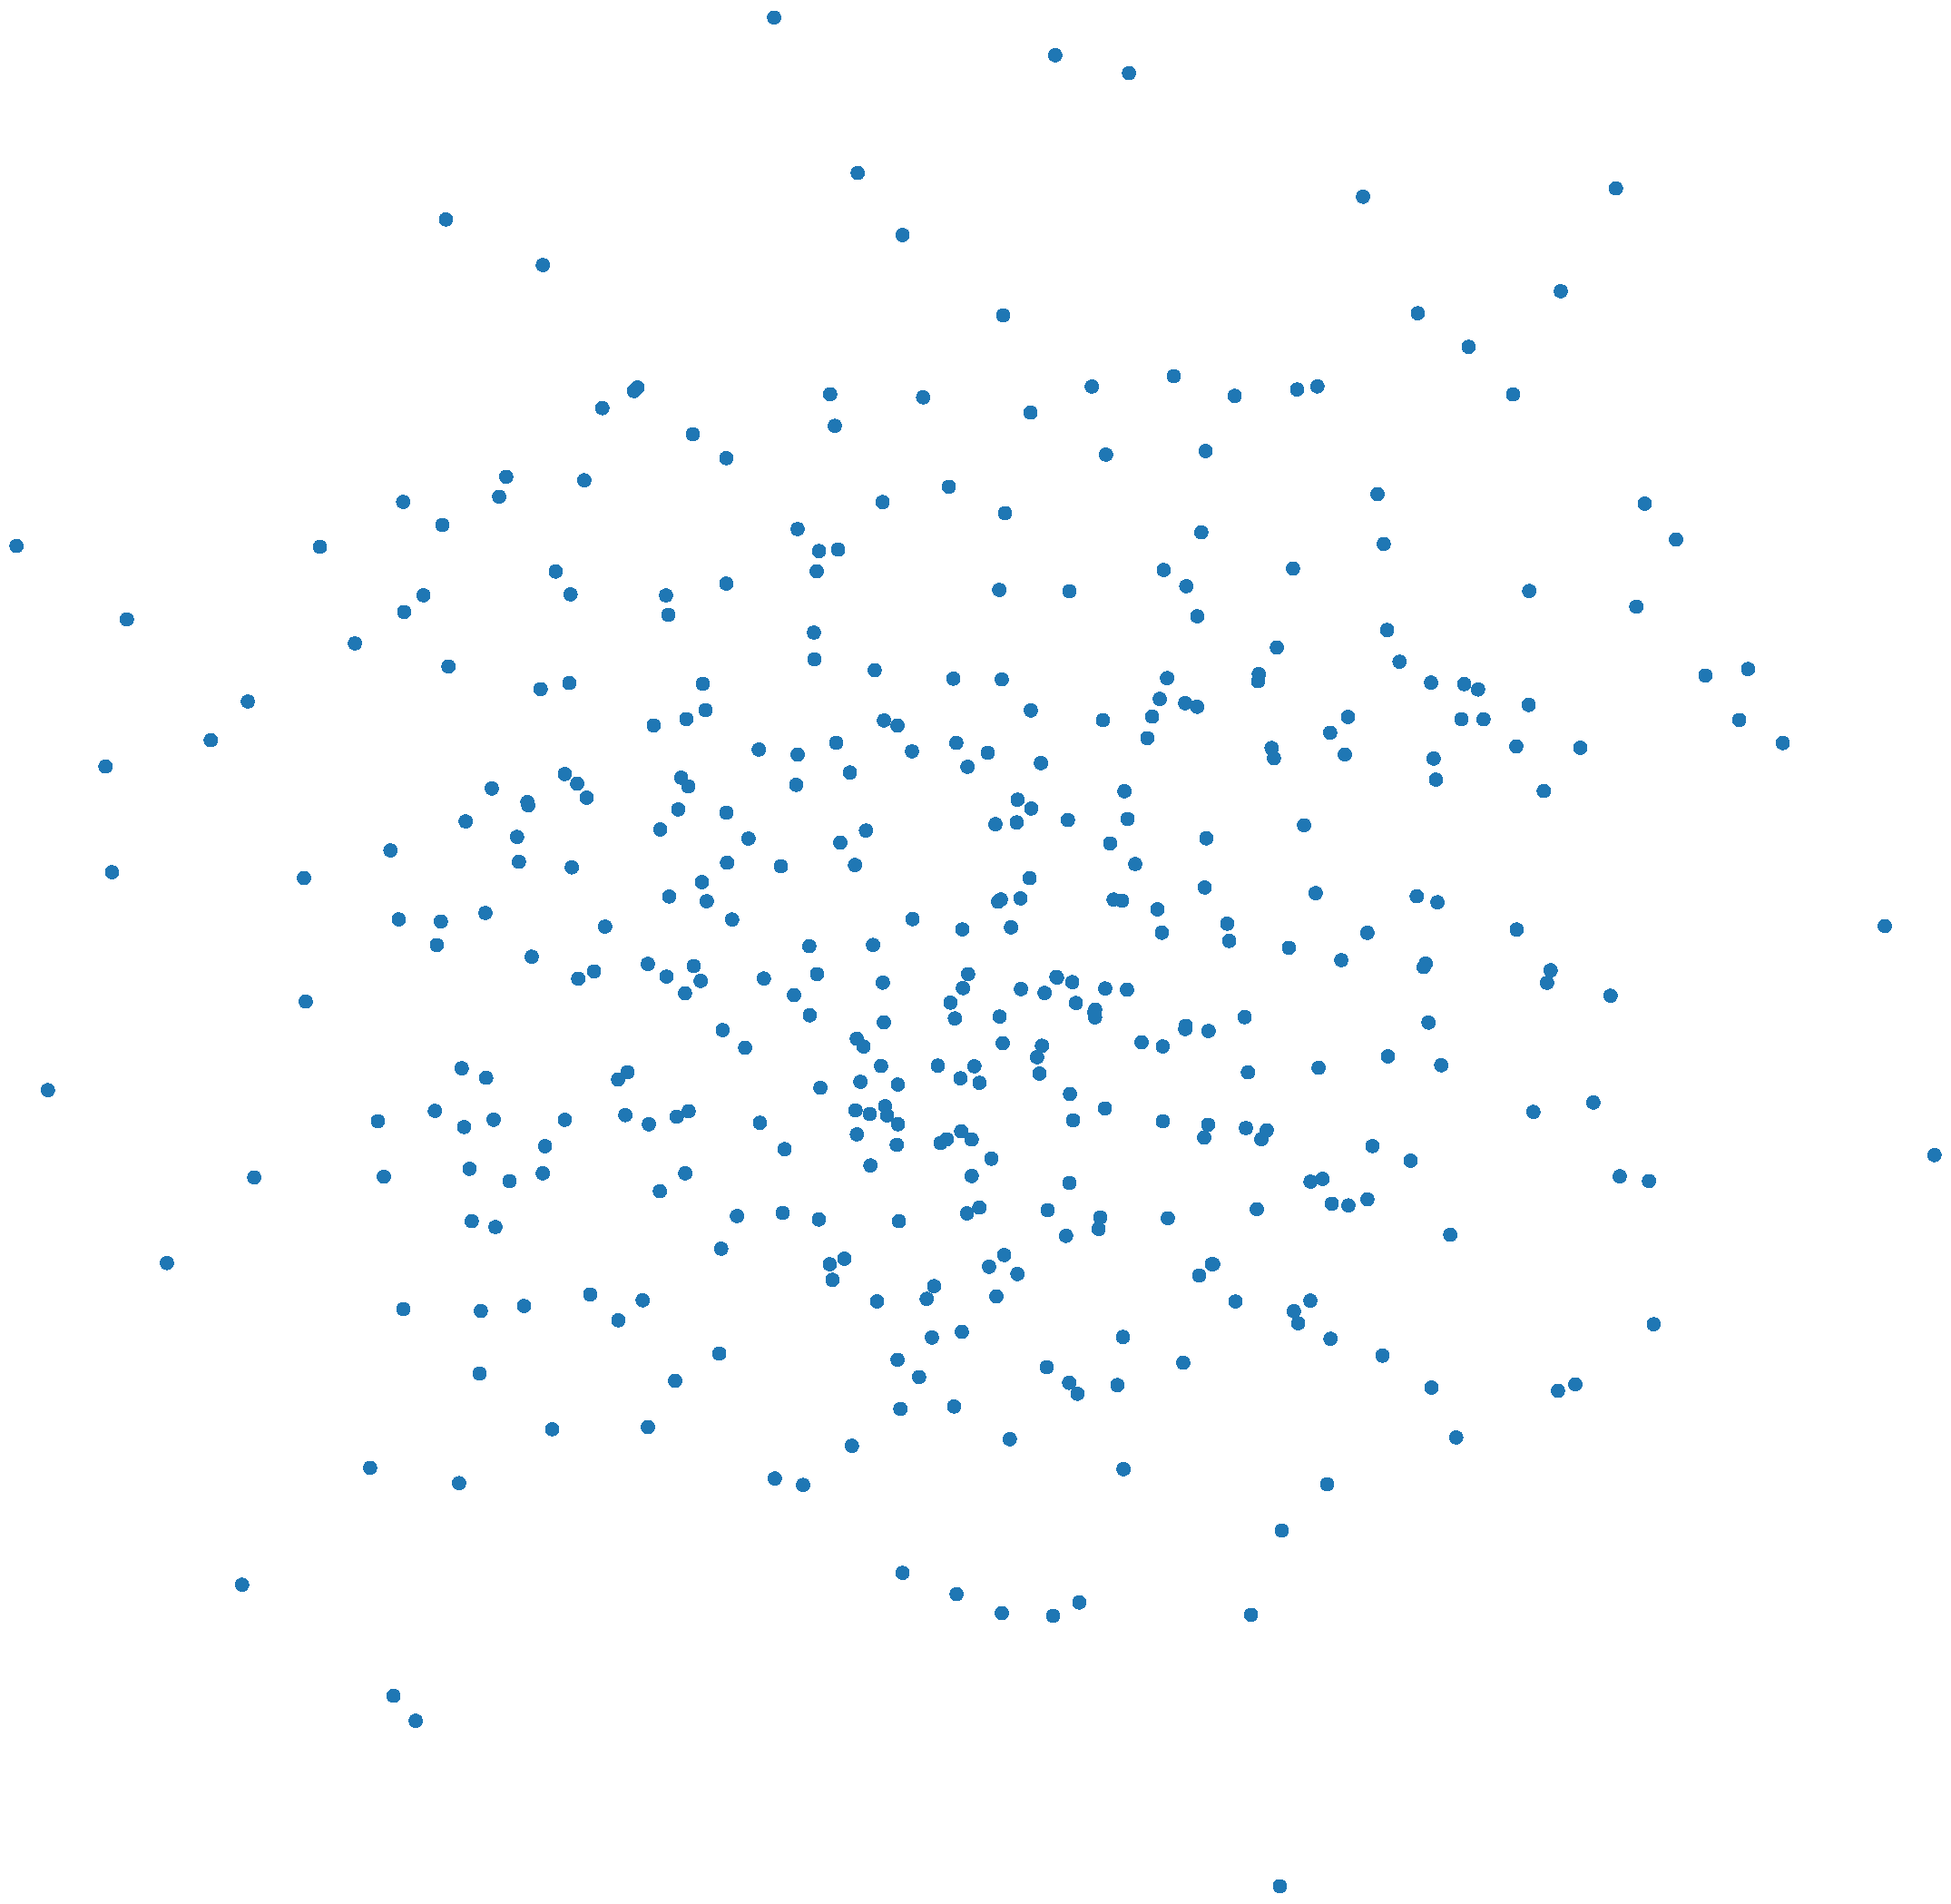
\includegraphics[width=.3\textwidth]{images/moon/zdist-crop.pdf}};
  \node[inner sep=0pt, right= 0.2cm of ffnn] (latentx) {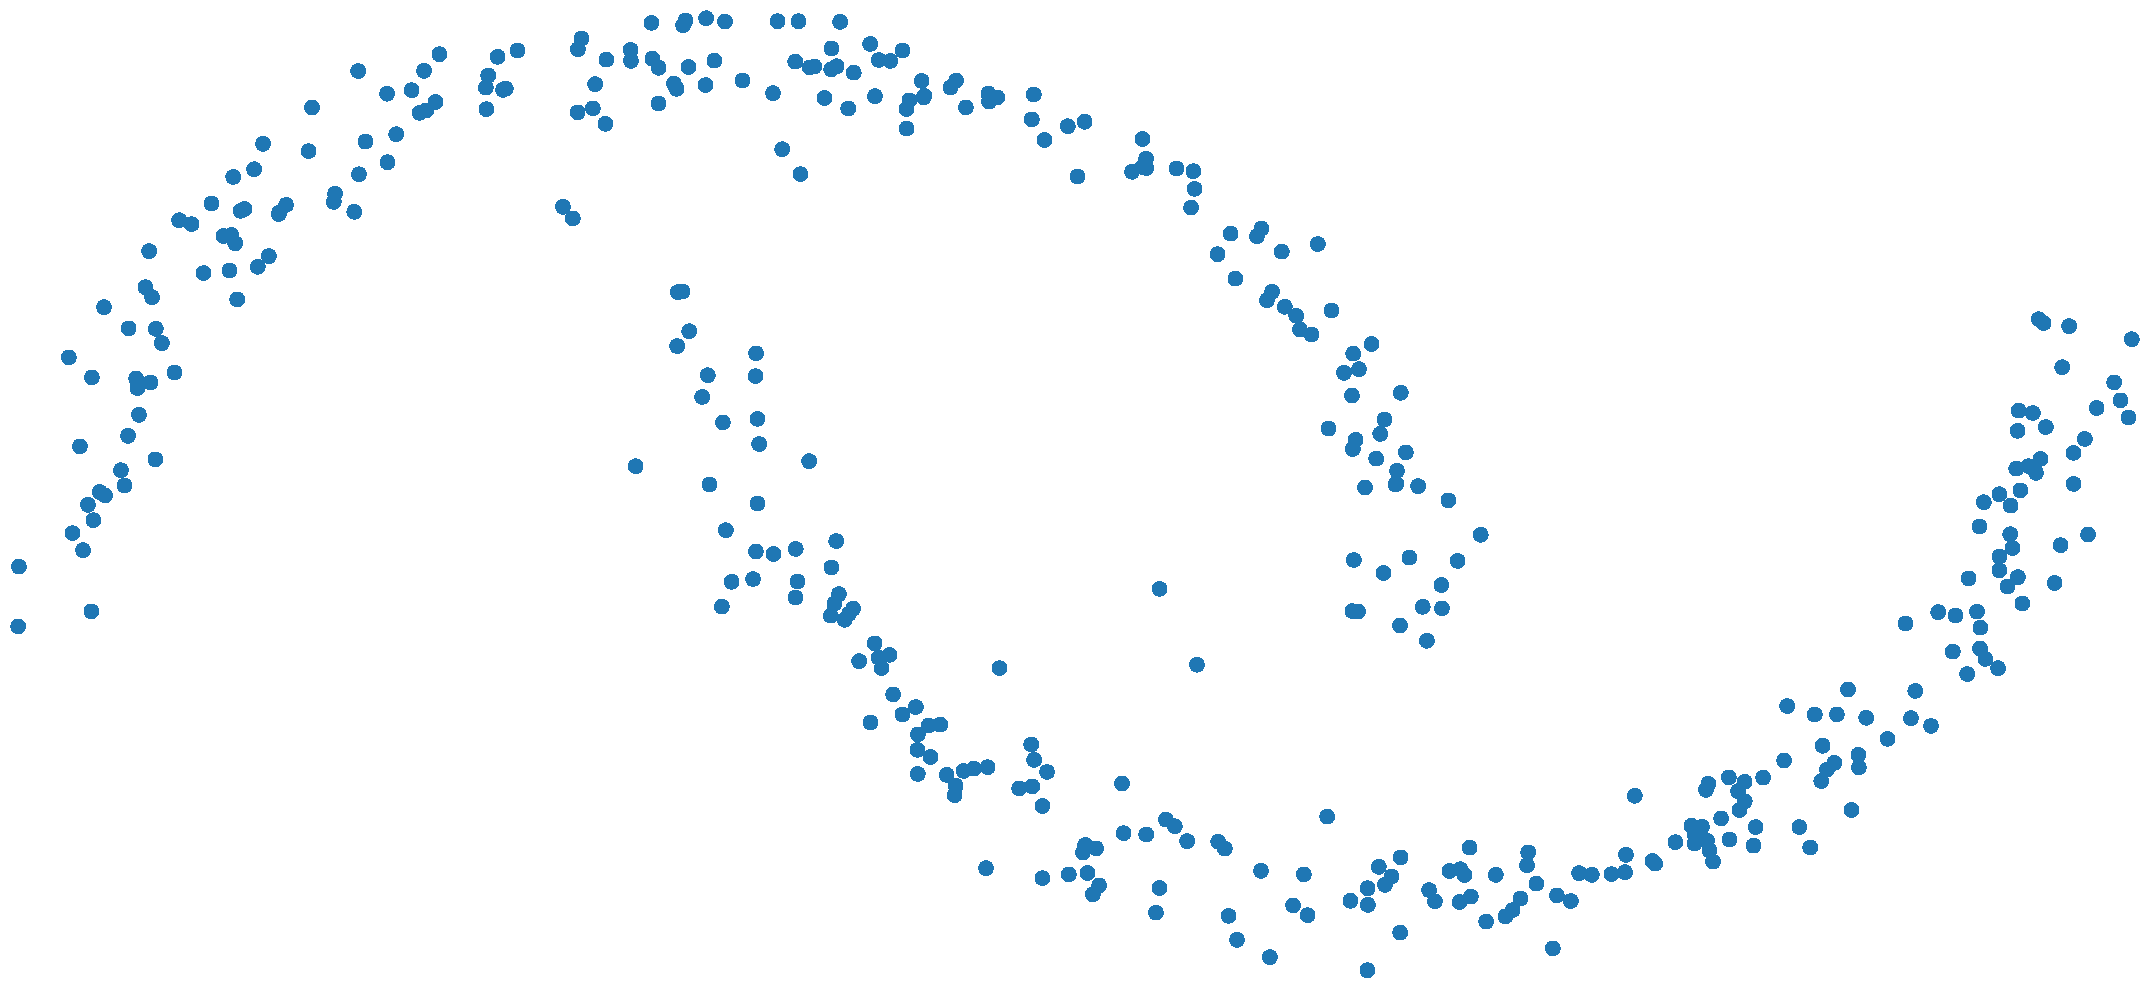
\includegraphics[width=.3\textwidth]{images/moon/xdist-crop.pdf}};
  
\end{scope}
%%% Local Variables:
%%% mode: latex
%%% TeX-master: "../ppgm_slide"
%%% End:

    \end{scope}
    
    \draw[dashed, ->, shorten >=5pt, shorten <=5pt, opacity=\bgopacity] ($(gk.north)+(0,-1.0cm)$) -- ($(gk.north)+(0,-2.0cm)$);
    
    %%%%%%%%%%%%%%%%%%%%%%%%%%%%%%%%%%%%%%%% 
    %% 4. one layer mapping of the flow
    %%%%%%%%%%%%%%%%%%%%%%%%%%%%%%%%%%%%%%%% 
    \draw[dashed, ->, shorten >=5pt, shorten <=5pt, opacity=\bgopacity] ($(latentz.west)+(-0.1cm,0)$) -- ($(latentz.west)+(-1.5cm,0)$);
    
    \begin{scope}[shift={($(dgm.south)+(0,-3.5cm)$)}, scale=0.5, every node/.append style={transform shape}, local bounding box=oneLayer, opacity=\bgopacity]
      % \tikzstyle{enode} = [thick, draw=blue, circle, inner sep = 3pt,
% align=center]
\tikzstyle{enode} = [thick, draw=black, circle, inner sep = 0, minimum size = 1cm,  align=center]
\tikzstyle{nnode} = [thick, rectangle, rounded corners = 2pt,minimum size = 0.4cm,draw,inner sep = 2pt]
\node[enode] (hal) at (-2,1) {$\bm{h}_{l,a}$};
\node[enode] (hbl) at (-2,-1) {$\bm{h}_{l,b}$};
\node[enode] (hal-1) at (2,1) {$\bm{h}_{l-1,a}$};
\node[enode] (hbl-1) at (2,-1) {$\bm{h}_{l-1,b}$};
\node[nnode] (times) at (-0.5,-1) {$\times$};
\node[nnode] (plus) at (0.5,-1) {$+$};
\node[nnode] (eq) at (0,1) {$=$};
\draw[->] (hal) -- node[fill=white] {$m_a$} (times);
\draw[->] (hal) -- node[fill=white] {$m_b$} (plus);
\draw[->] (hal) to (eq);

\draw[->] (eq) to (hal-1);
\draw[->] (hbl) to (times);
\draw[->] (times) to (plus);
\draw[->] (plus) to (hbl-1);
% \draw[draw=black] (-0.5,-0.5) rectangle ++(1,2);

%%% Local Variables:
%%% mode: latex
%%% TeX-master: "../ppgm_slide"
%%% End:

    \end{scope}
    
  \end{tikzpicture}
\end{frame}


\begin{frame}[label=current]{A High-level View of GenMM: flow gears}
  \begin{tikzpicture}
    \tikzstyle{enode} = [thick, draw=black, circle, align=center]
    \tikzstyle{cnode} = [thick, draw=black, circle, align=center, inner sep = 0.3pt]
    \tikzstyle{nnode} = [thick, rectangle, rounded corners = 2pt,minimum size = 0.8cm,draw,inner sep = 22pt]
    %%%%%%%%%%%%%%%%%%%%%%%%%%%%%%%%%%%%%%%% 
    %% 1. directed graphical model
    %%%%%%%%%%%%%%%%%%%%%%%%%%%%%%%%%%%%%%%% 
    \begin{scope}[scale=0.4, every node/.append style={transform shape}, local bounding box=dgm, opacity=0.3]
      \node[enode] (x) at (0,0){$\bm{x}$};

\node[enode, above=of x] (s) {$\bm{s}$};
\node[enode, left=of s] (z) {$\bm{z}$};
\node[enode, right=of s] (pi) {$\bm{\pi}$};
\node[cnode, right=of x] (phi) {$\{ \bm{\theta}_k \}$};
\node[nnode, fit=(x)(z)(s)] (box) {};

\draw[->] (z) to (x);
\draw[->] (s) to (x);
\draw[->] (pi) to (s);
\draw[->] (phi) to (x);

%%% Local Variables:
%%% mode: latex
%%% TeX-master: "../ppgm_slide"
%%% End:

    \end{scope}
    
    %%%%%%%%%%%%%%%%%%%%%%%%%%%%%%%%%%%%%%%% 
    %% 2. illustration of GenMM
    %%%%%%%%%%%%%%%%%%%%%%%%%%%%%%%%%%%%%%%% 
    \begin{scope}[scale=0.3, every node/.append style={transform shape}, shift={($(dgm.east)+(16cm,0)$)}, local bounding box=illsGenMM, opacity=\bgopacity]
      
% \tikzstyle{enode} = [thick, draw=blue, circle, inner sep = 3pt,
% align=center]
\tikzstyle{enode} = [thick, draw=black, ellipse, inner sep = 2pt,  align=center]
\tikzstyle{nnode} = [thick, rectangle, rounded corners = 2pt,minimum size = 0.8cm,draw,inner sep = 2pt]
\node[enode,label={below:{\tiny Shared latent source}}] (z) at (0,0) {$\bm{z}\sim p(\bm{z})$};
\node[enode, label={below:{\tiny Induced distribution}}] (x) at (5.5,0){$\bm{x}\sim p(\bm{x}; \bm{\Phi})$};
% \node at (5.2,-1) {$p(\bm{x};\bm{\Phi}) = \textstyle\sum_{k=1}^K \pi_k  p_k(\bm{x})$};
\node[nnode] (g1) at (2.6,1.8) {$\bm{g}_1$};
\node[nnode] (g2) at (2.6,0.5) {$\bm{g}_2$};
\node[nnode] (gk) at (2.6,-1.8) {$\bm{g}_K$};
\draw[dotted,line width=2pt] (2.6,-0.3) -- (2.6,-1.2);
\draw[->] (z) [in= 180, out =0] to (g1);
\draw[->] (z) [in= 180, out =0] to (g2);
\draw[->] (z) [in= 180, out =0] to (gk);
\filldraw[->] (3.7, 0.5)circle (2pt) -- node[above=0.2](switch){$\bm{s}\sim \bm{\pi}$} (x);
\node[above= 0.2 of switch.east] {\tiny \begin{tabular}{c}Categorical variable\\ as generator switch\end{tabular}};
% \draw[->] (3,-0.8) -- (3.5, -0.8);
\draw[->] (g1) -- (3.5,1.8);
\draw[->] (g2) -- (3.5, 0.5);
\draw[->] (gk) -- (3.5, -1.8);
\begin{scope}[on background layer, every node/.append style={transform shape}]
\node [rounded corners = 2pt, inner sep=4pt, fill=blue!30,fit=(g1)(g2)(gk), label={[label distance=0.3cm]-60:{\tiny Mixture of generators}}] {};
\end{scope}
%%% Local Variables:
%%% mode: latex
%%% TeX-master: "../ppgm_slide"
%%% End:

    \end{scope}
    \draw[dashed, ->, shorten >=5pt, shorten <=5pt, opacity=\bgopacity] (dgm) --node [text width=2cm, black, midway,above]{} (illsGenMM);
    
    %%%%%%%%%%%%%%%%%%%%%%%%%%%%%%%%%%%%%%%% 
    %% 3. illustration of flow
    %%%%%%%%%%%%%%%%%%%%%%%%%%%%%%%%%%%%%%%% 

    \begin{scope}[shift={($(illsGenMM.south)+(-0.5cm,0cm)$)}, scale=0.8, local bounding box=illFlow]
      \def\layersep{1.5cm}
\begin{scope}[shorten >=1pt,->,draw=black!50, node distance=\layersep, scale=0.6, every node/.append style={transform shape},transform shape, local bounding box=ffnn]
  \tikzstyle{every pin edge}=[<-,shorten <=1pt]
  \tikzstyle{neuron}=[circle,fill=black!50,minimum size=17pt,inner sep=0pt]
  \tikzstyle{input neuron}=[neuron, fill=green!80];
  \tikzstyle{output neuron}=[neuron, fill=red!80];
  \tikzstyle{hidden neuron}=[neuron, fill=blue!80];
  \tikzstyle{annot} = [text width=4em, text centered]

  % Draw the input layer nodes
  \foreach \name / \y in {1,...,4}
  % This is the same as writing \foreach \name / \y in {1/1,2/2,3/3,4/4}
  % \node[input neuron, pin=left:Input \#\y] (I-\name) at (0,-\y) {};
  \node[input neuron, pin=left:{}] (I-\name) at (0,-\y) {};


  % Draw the hidden layer nodes
  \foreach \name / \y in {1,...,4}
  \path[yshift=0.0cm] node[hidden neuron] (H-\name) at (\layersep,-\y cm) {};

  % Draw the output layer node
  \foreach \name / \y in {1,...,4}
  \node[output neuron,pin={[pin edge={->}]right:{}}] (O-\name) at (2*\layersep, -\y cm) {};

  % Connect every node in the input layer with every node in the
  % hidden layer.
  \foreach \source in {1,...,4}
  \foreach \dest in {1,...,4}
  \draw[-{Stealth[scale=0.5]}] (I-\source) edge (H-\dest);

  % Connect every node in the hidden layer with the output layer
  \foreach \source in {1,...,4}
  \foreach \dest in {1,...,4}
  \draw[-{Stealth[scale=0.5]}] (H-\source) edge (O-\dest);

  % \foreach \source in {1,...,4}
  % \path (H-\source) edge (O);

  % Annotate the layers
  % \node[annot,above of=H-1, node distance=1cm] (hl) {Hidden layer};
  % \node[annot,left of=hl] {Input layer};
  % \node[annot,right of=hl] {Output layer};
  \node[inner sep=0pt, left= 0.2cm of ffnn] (latentz) {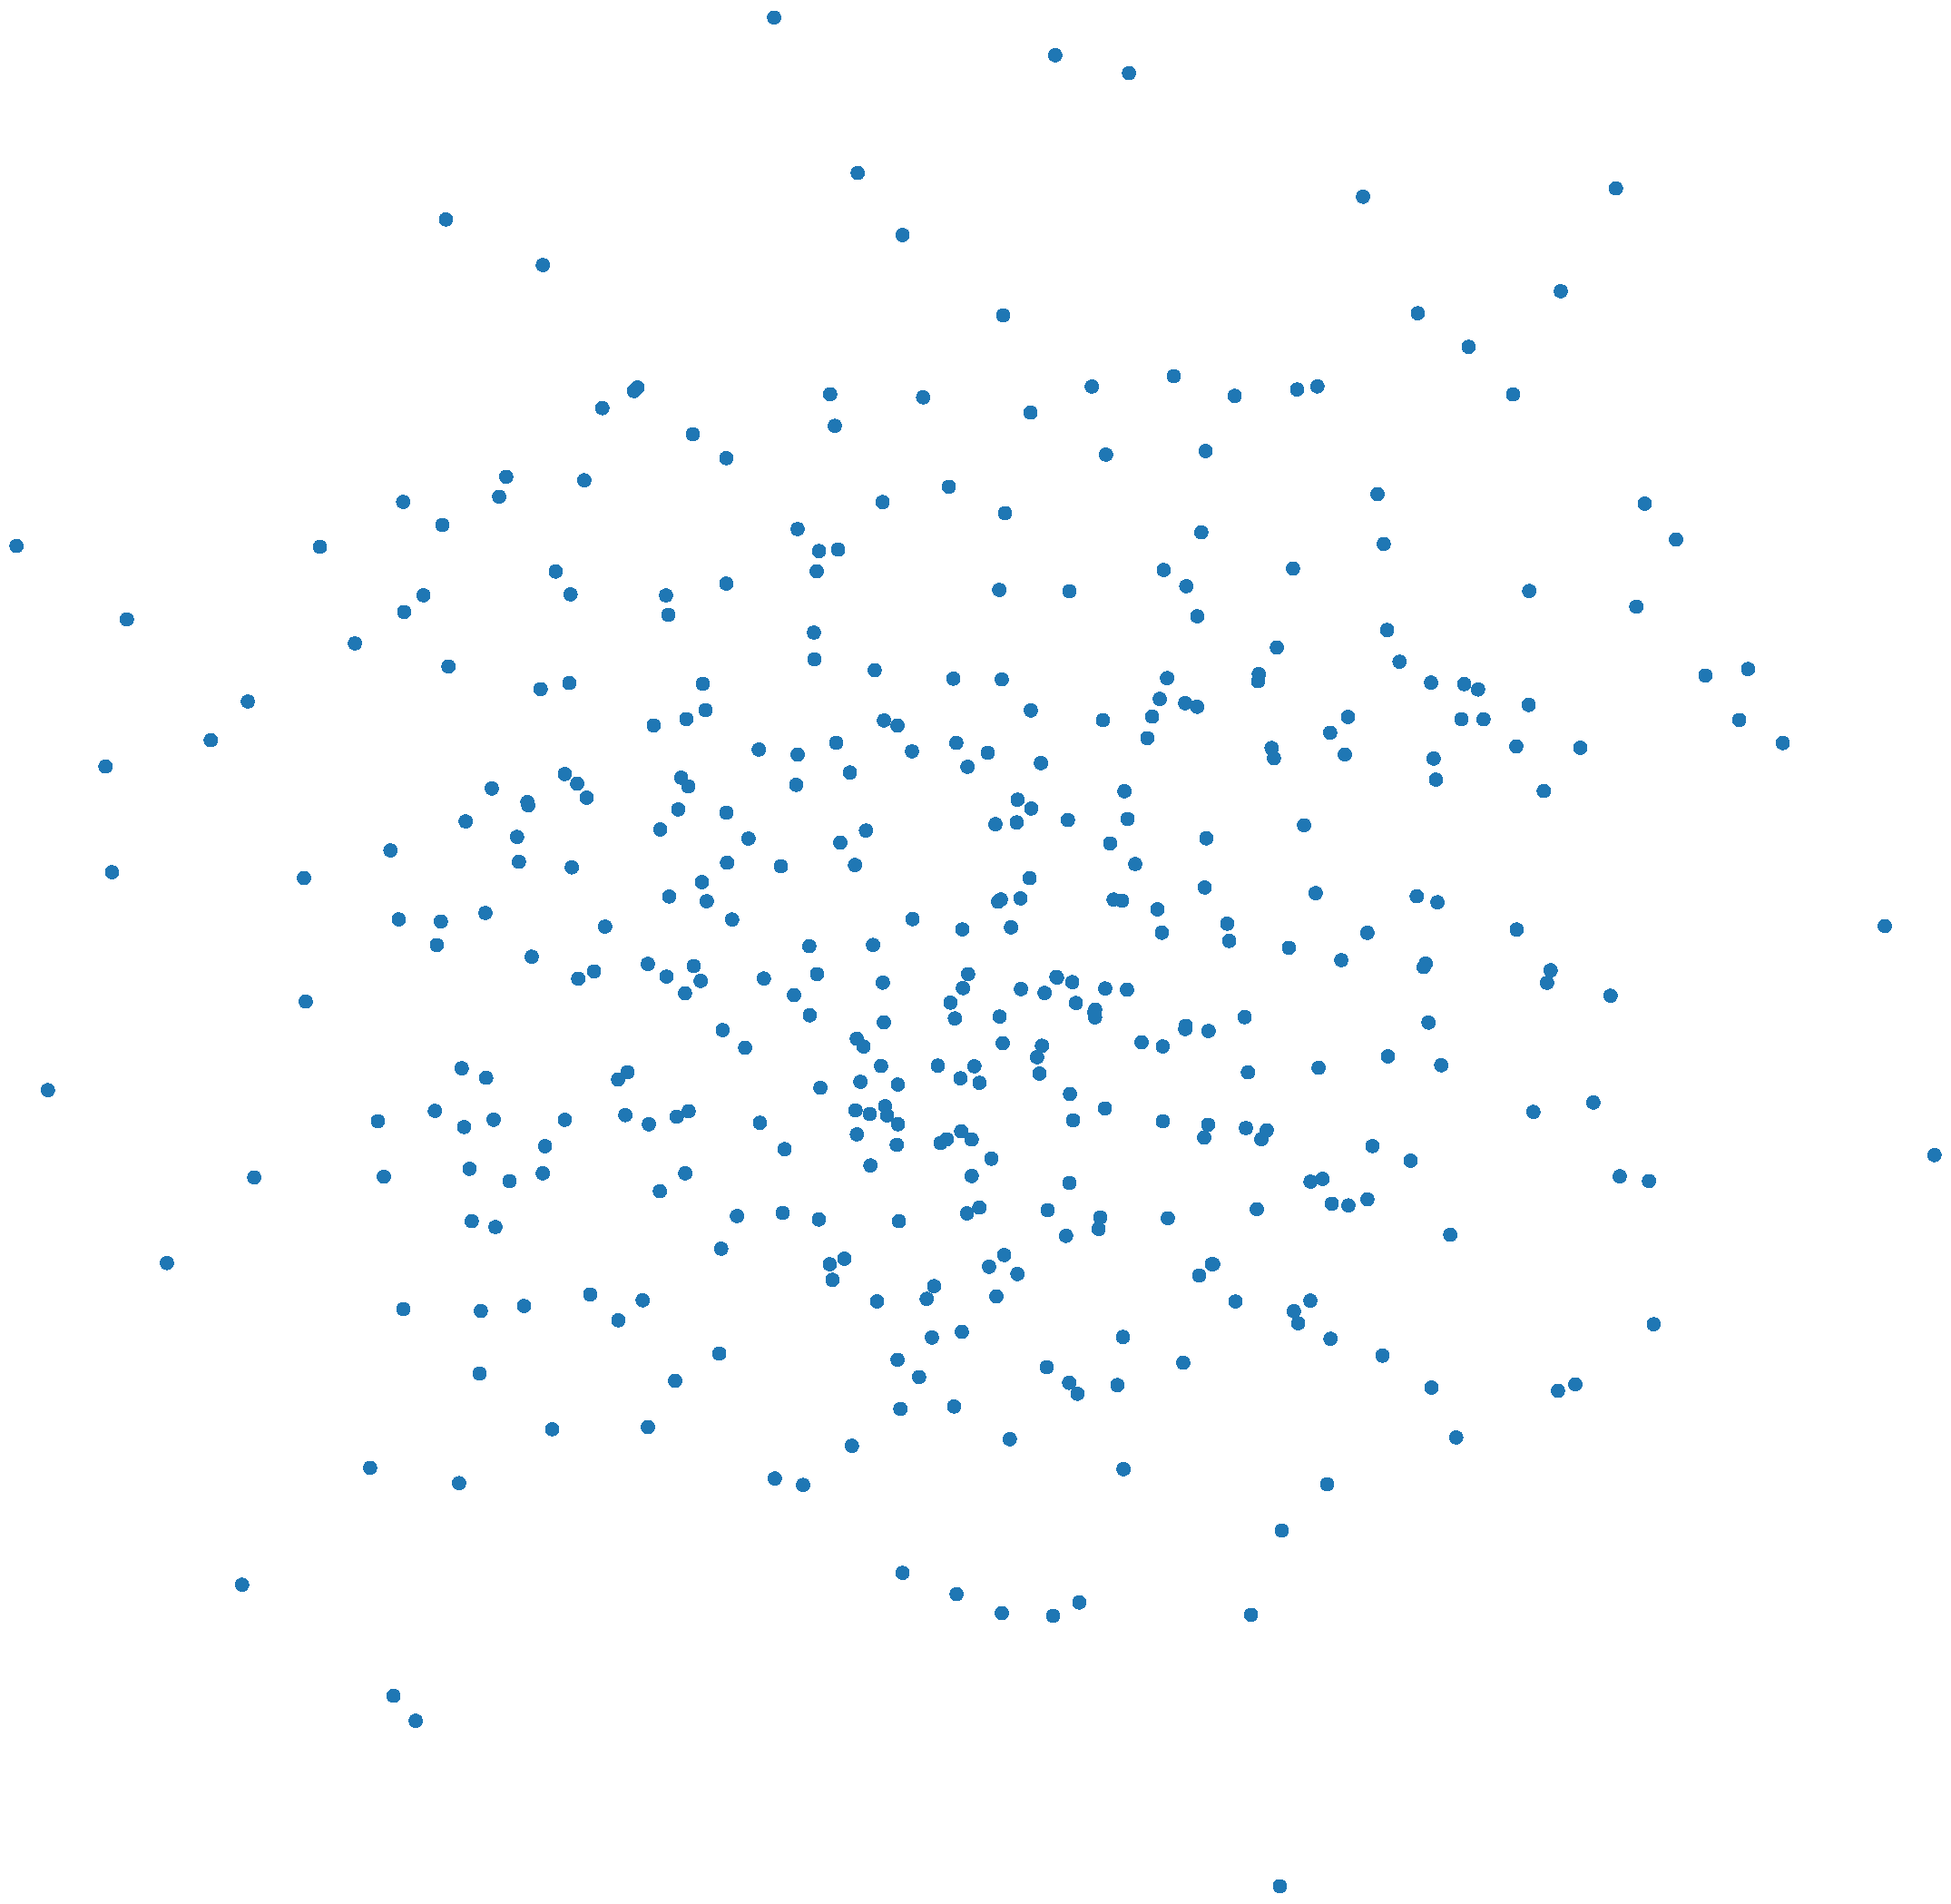
\includegraphics[width=.3\textwidth]{images/moon/zdist-crop.pdf}};
  \node[inner sep=0pt, right= 0.2cm of ffnn] (latentx) {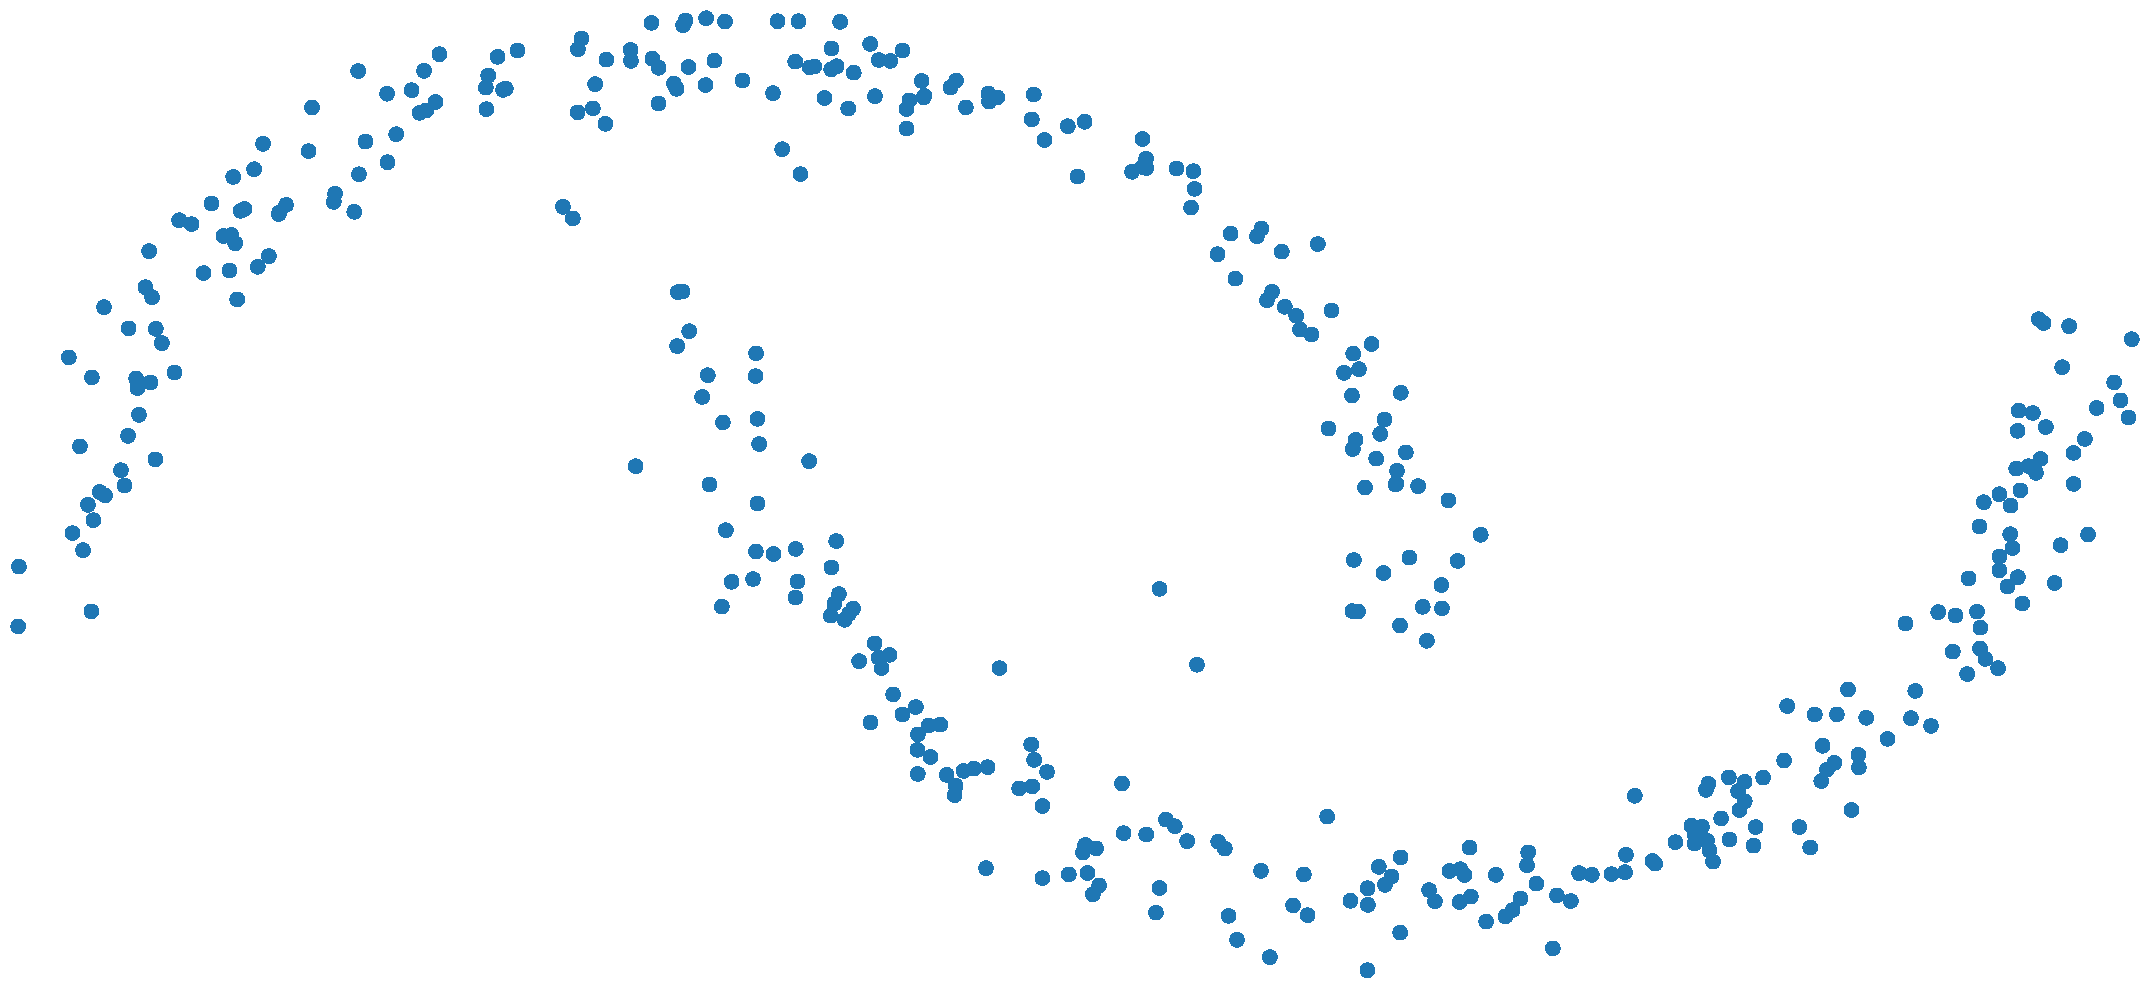
\includegraphics[width=.3\textwidth]{images/moon/xdist-crop.pdf}};
  
\end{scope}
%%% Local Variables:
%%% mode: latex
%%% TeX-master: "../ppgm_slide"
%%% End:

    \end{scope}
    \node [black, below=-0.05cm of illFlow] (changeveq) {
      \scriptsize
      \begin{minipage}{0.7\textwidth}
        When the $k$-th generator is selected, i.e., $s_k=1$ and $s_{k^{\prime}}=0$  for $k^{\prime}\neq k$, say $\tilde{\bm{x}} = \bm{x}|_{s_k=1}$. By following the \href{https://online.stat.psu.edu/stat414/lesson/23/23.1}{change of variable rule}
        \vskip -0.4cm
        \begin{equation*}
          \underbrace{p(\tilde{\bm{x}})|_{\tilde{\bm{x}} = \tilde{\bm{g}}(\bm{z})}}_{\text{Induced distribution}} =  \underbrace{p(\bm{z})}_{\text{\begin{tabular}{c}Assumed known distribution \\ easy to sample\end{tabular}}}\cdot \underbrace{\bigg| \mathrm{det}\left({\pd{\bm{z}}{\tilde{\bm{x}}}}\right)\bigg|}_{\text{\begin{tabular}{c}Computational load\\ depends on the mapping\end{tabular}}}.
        \end{equation*}
        \only<1>{
          \vskip -0.4cm
          A toy example:\\
        }
        \only<2>{
          \vskip -0.4cm
          Powering it with a $L$-layer neural network implementation:
        }
      \end{minipage}};
    \draw[green, ->, shorten >=5pt, shorten <=5pt] ($(gk.north)+(0,0cm)$) -- ($(gk.north)+(0,-0.8cm)$);
    \only<1>{
      \begin{scope}[scale=0.8, shift={($(changeveq.south)+(-2.5cm,-0.7cm)$)}]
        \node[black] at (2.5cm, 0) {\scriptsize
          Gaussian linear transform: $Z \sim \mathsf{N}\left( 0, 1  \right)$ $\xrightarrow{X=\sigma\cdot Z + \mu}$ $X \sim \mathsf{N}\left( \mu, \sigma  \right)$
        };
      \end{scope}
    }
    \only<2>{
      \begin{scope}[scale=0.8, shift={($(changeveq.south)+(-2.5cm,-0.7cm)$)}]
        \node (z) at (0,0) {};
        \node at ($(z)-(0.5,0)$){$\bm{z}=\bm{h}_0$};
        \node (xi1) at (1.5,0) {$\bm{h}_1$};
        \node (xi2) at (3,0) {};
        \node (xi3) at (4.5,0){};
        \node (x) at (6,0) {};
        \node at ($(x)+(0.5,0)$){$\bm{x} = \bm{h}_L$};
        \draw[->] ($(z) + (0.3,0.1)$) -- node[above]{$\tilde{\bm{g}}_1$} ($(xi1)+(-0.3,0.1)$); 
        \draw[->] ($(xi1)-(0.3,0.1)$) -- node[below]{$\tilde{\bm{f}}_1$}($(z) - (-0.3,0.1)$);
        \draw[->] ($(xi1) + (0.3,0.1)$) -- node[above]{$\tilde{\bm{g}}_2$} ($(xi2)+(-0.3,0.1)$); 
        \draw[->] ($(xi2)-(0.3,0.1)$) -- node[below]{$\tilde{\bm{f}}_2$}($(xi1) - (-0.3,0.1)$);
        \draw[->] ($(xi3) + (0.3,0.1)$) -- node[above]{$\tilde{\bm{g}}_L$} ($(x)+(-0.3,0.1)$); 
        \draw[->] ($(x)-(0.3,0.1)$) -- node[below]{$\tilde{\bm{f}}_L$}($(xi3) - (-0.3,0.1)$);
        \draw[dotted,line width = 0.3 mm] (xi2) -- (xi3);
      \end{scope}
    }
    %%%%%%%%%%%%%%%%%%%%%%%%%%%%%%%%%%%%%%%% 
    %% 4. one layer mapping of the flow
    %%%%%%%%%%%%%%%%%%%%%%%%%%%%%%%%%%%%%%%% 
    
    \begin{scope}[shift={($(dgm.south)+(0,-3.5cm)$)}, scale=0.3, every node/.append style={transform shape}, local bounding box=oneLayer, opacity=\bgopacity]
      % \tikzstyle{enode} = [thick, draw=blue, circle, inner sep = 3pt,
% align=center]
\tikzstyle{enode} = [thick, draw=black, circle, inner sep = 0, minimum size = 1cm,  align=center]
\tikzstyle{nnode} = [thick, rectangle, rounded corners = 2pt,minimum size = 0.4cm,draw,inner sep = 2pt]
\node[enode] (hal) at (-2,1) {$\bm{h}_{l,a}$};
\node[enode] (hbl) at (-2,-1) {$\bm{h}_{l,b}$};
\node[enode] (hal-1) at (2,1) {$\bm{h}_{l-1,a}$};
\node[enode] (hbl-1) at (2,-1) {$\bm{h}_{l-1,b}$};
\node[nnode] (times) at (-0.5,-1) {$\times$};
\node[nnode] (plus) at (0.5,-1) {$+$};
\node[nnode] (eq) at (0,1) {$=$};
\draw[->] (hal) -- node[fill=white] {$m_a$} (times);
\draw[->] (hal) -- node[fill=white] {$m_b$} (plus);
\draw[->] (hal) to (eq);

\draw[->] (eq) to (hal-1);
\draw[->] (hbl) to (times);
\draw[->] (times) to (plus);
\draw[->] (plus) to (hbl-1);
% \draw[draw=black] (-0.5,-0.5) rectangle ++(1,2);

%%% Local Variables:
%%% mode: latex
%%% TeX-master: "../ppgm_slide"
%%% End:

    \end{scope}
    \draw[dashed, ->, shorten >=5pt, shorten <=5pt, opacity=\bgopacity] ($(oneLayer.east)+(1.5cm,0cm)$) -- ($(oneLayer.east)+(0.1cm,0)$);
    
  \end{tikzpicture}
\end{frame}



\begin{frame}[label=current]{A High-level View of GenMM: Zoom into Layer}
  \begin{tikzpicture}
    \tikzstyle{enode} = [thick, draw=black, circle, align=center]
    \tikzstyle{cnode} = [thick, draw=black, circle, align=center, inner sep = 0.3pt]
    \tikzstyle{nnode} = [thick, rectangle, rounded corners = 2pt,minimum size = 0.8cm,draw,inner sep = 22pt]
    %%%%%%%%%%%%%%%%%%%%%%%%%%%%%%%%%%%%%%%% 
    %% 1. directed graphical model
    %%%%%%%%%%%%%%%%%%%%%%%%%%%%%%%%%%%%%%%% 
    \begin{scope}[scale=0.4, every node/.append style={transform shape}, local bounding box=dgm, opacity=0.3]
      \node[enode] (x) at (0,0){$\bm{x}$};

\node[enode, above=of x] (s) {$\bm{s}$};
\node[enode, left=of s] (z) {$\bm{z}$};
\node[enode, right=of s] (pi) {$\bm{\pi}$};
\node[cnode, right=of x] (phi) {$\{ \bm{\theta}_k \}$};
\node[nnode, fit=(x)(z)(s)] (box) {};

\draw[->] (z) to (x);
\draw[->] (s) to (x);
\draw[->] (pi) to (s);
\draw[->] (phi) to (x);

%%% Local Variables:
%%% mode: latex
%%% TeX-master: "../ppgm_slide"
%%% End:

    \end{scope}
    
    %%%%%%%%%%%%%%%%%%%%%%%%%%%%%%%%%%%%%%%% 
    %% 2. illustration of GenMM
    %%%%%%%%%%%%%%%%%%%%%%%%%%%%%%%%%%%%%%%% 
    \begin{scope}[scale=0.3, every node/.append style={transform shape}, shift={($(dgm.east)+(20cm,0)$)}, local bounding box=illsGenMM, opacity=\bgopacity]
      
% \tikzstyle{enode} = [thick, draw=blue, circle, inner sep = 3pt,
% align=center]
\tikzstyle{enode} = [thick, draw=black, ellipse, inner sep = 2pt,  align=center]
\tikzstyle{nnode} = [thick, rectangle, rounded corners = 2pt,minimum size = 0.8cm,draw,inner sep = 2pt]
\node[enode,label={below:{\tiny Shared latent source}}] (z) at (0,0) {$\bm{z}\sim p(\bm{z})$};
\node[enode, label={below:{\tiny Induced distribution}}] (x) at (5.5,0){$\bm{x}\sim p(\bm{x}; \bm{\Phi})$};
% \node at (5.2,-1) {$p(\bm{x};\bm{\Phi}) = \textstyle\sum_{k=1}^K \pi_k  p_k(\bm{x})$};
\node[nnode] (g1) at (2.6,1.8) {$\bm{g}_1$};
\node[nnode] (g2) at (2.6,0.5) {$\bm{g}_2$};
\node[nnode] (gk) at (2.6,-1.8) {$\bm{g}_K$};
\draw[dotted,line width=2pt] (2.6,-0.3) -- (2.6,-1.2);
\draw[->] (z) [in= 180, out =0] to (g1);
\draw[->] (z) [in= 180, out =0] to (g2);
\draw[->] (z) [in= 180, out =0] to (gk);
\filldraw[->] (3.7, 0.5)circle (2pt) -- node[above=0.2](switch){$\bm{s}\sim \bm{\pi}$} (x);
\node[above= 0.2 of switch.east] {\tiny \begin{tabular}{c}Categorical variable\\ as generator switch\end{tabular}};
% \draw[->] (3,-0.8) -- (3.5, -0.8);
\draw[->] (g1) -- (3.5,1.8);
\draw[->] (g2) -- (3.5, 0.5);
\draw[->] (gk) -- (3.5, -1.8);
\begin{scope}[on background layer, every node/.append style={transform shape}]
\node [rounded corners = 2pt, inner sep=4pt, fill=blue!30,fit=(g1)(g2)(gk), label={[label distance=0.3cm]-60:{\tiny Mixture of generators}}] {};
\end{scope}
%%% Local Variables:
%%% mode: latex
%%% TeX-master: "../ppgm_slide"
%%% End:

    \end{scope}
    \draw[dashed, ->, shorten >=5pt, shorten <=5pt, opacity=\bgopacity] (dgm) --node [text width=2cm, black, midway,above]{} (illsGenMM);
    
    %%%%%%%%%%%%%%%%%%%%%%%%%%%%%%%%%%%%%%%% 
    %% 3. illustration of flow
    %%%%%%%%%%%%%%%%%%%%%%%%%%%%%%%%%%%%%%%% 

    \begin{scope}[shift={($(illsGenMM.south)+(-0.5cm,0cm)$)}, scale=0.5, local bounding box=illFlow, opacity=\bgopacity]
      \def\layersep{1.5cm}
\begin{scope}[shorten >=1pt,->,draw=black!50, node distance=\layersep, scale=0.6, every node/.append style={transform shape},transform shape, local bounding box=ffnn]
  \tikzstyle{every pin edge}=[<-,shorten <=1pt]
  \tikzstyle{neuron}=[circle,fill=black!50,minimum size=17pt,inner sep=0pt]
  \tikzstyle{input neuron}=[neuron, fill=green!80];
  \tikzstyle{output neuron}=[neuron, fill=red!80];
  \tikzstyle{hidden neuron}=[neuron, fill=blue!80];
  \tikzstyle{annot} = [text width=4em, text centered]

  % Draw the input layer nodes
  \foreach \name / \y in {1,...,4}
  % This is the same as writing \foreach \name / \y in {1/1,2/2,3/3,4/4}
  % \node[input neuron, pin=left:Input \#\y] (I-\name) at (0,-\y) {};
  \node[input neuron, pin=left:{}] (I-\name) at (0,-\y) {};


  % Draw the hidden layer nodes
  \foreach \name / \y in {1,...,4}
  \path[yshift=0.0cm] node[hidden neuron] (H-\name) at (\layersep,-\y cm) {};

  % Draw the output layer node
  \foreach \name / \y in {1,...,4}
  \node[output neuron,pin={[pin edge={->}]right:{}}] (O-\name) at (2*\layersep, -\y cm) {};

  % Connect every node in the input layer with every node in the
  % hidden layer.
  \foreach \source in {1,...,4}
  \foreach \dest in {1,...,4}
  \draw[-{Stealth[scale=0.5]}] (I-\source) edge (H-\dest);

  % Connect every node in the hidden layer with the output layer
  \foreach \source in {1,...,4}
  \foreach \dest in {1,...,4}
  \draw[-{Stealth[scale=0.5]}] (H-\source) edge (O-\dest);

  % \foreach \source in {1,...,4}
  % \path (H-\source) edge (O);

  % Annotate the layers
  % \node[annot,above of=H-1, node distance=1cm] (hl) {Hidden layer};
  % \node[annot,left of=hl] {Input layer};
  % \node[annot,right of=hl] {Output layer};
  \node[inner sep=0pt, left= 0.2cm of ffnn] (latentz) {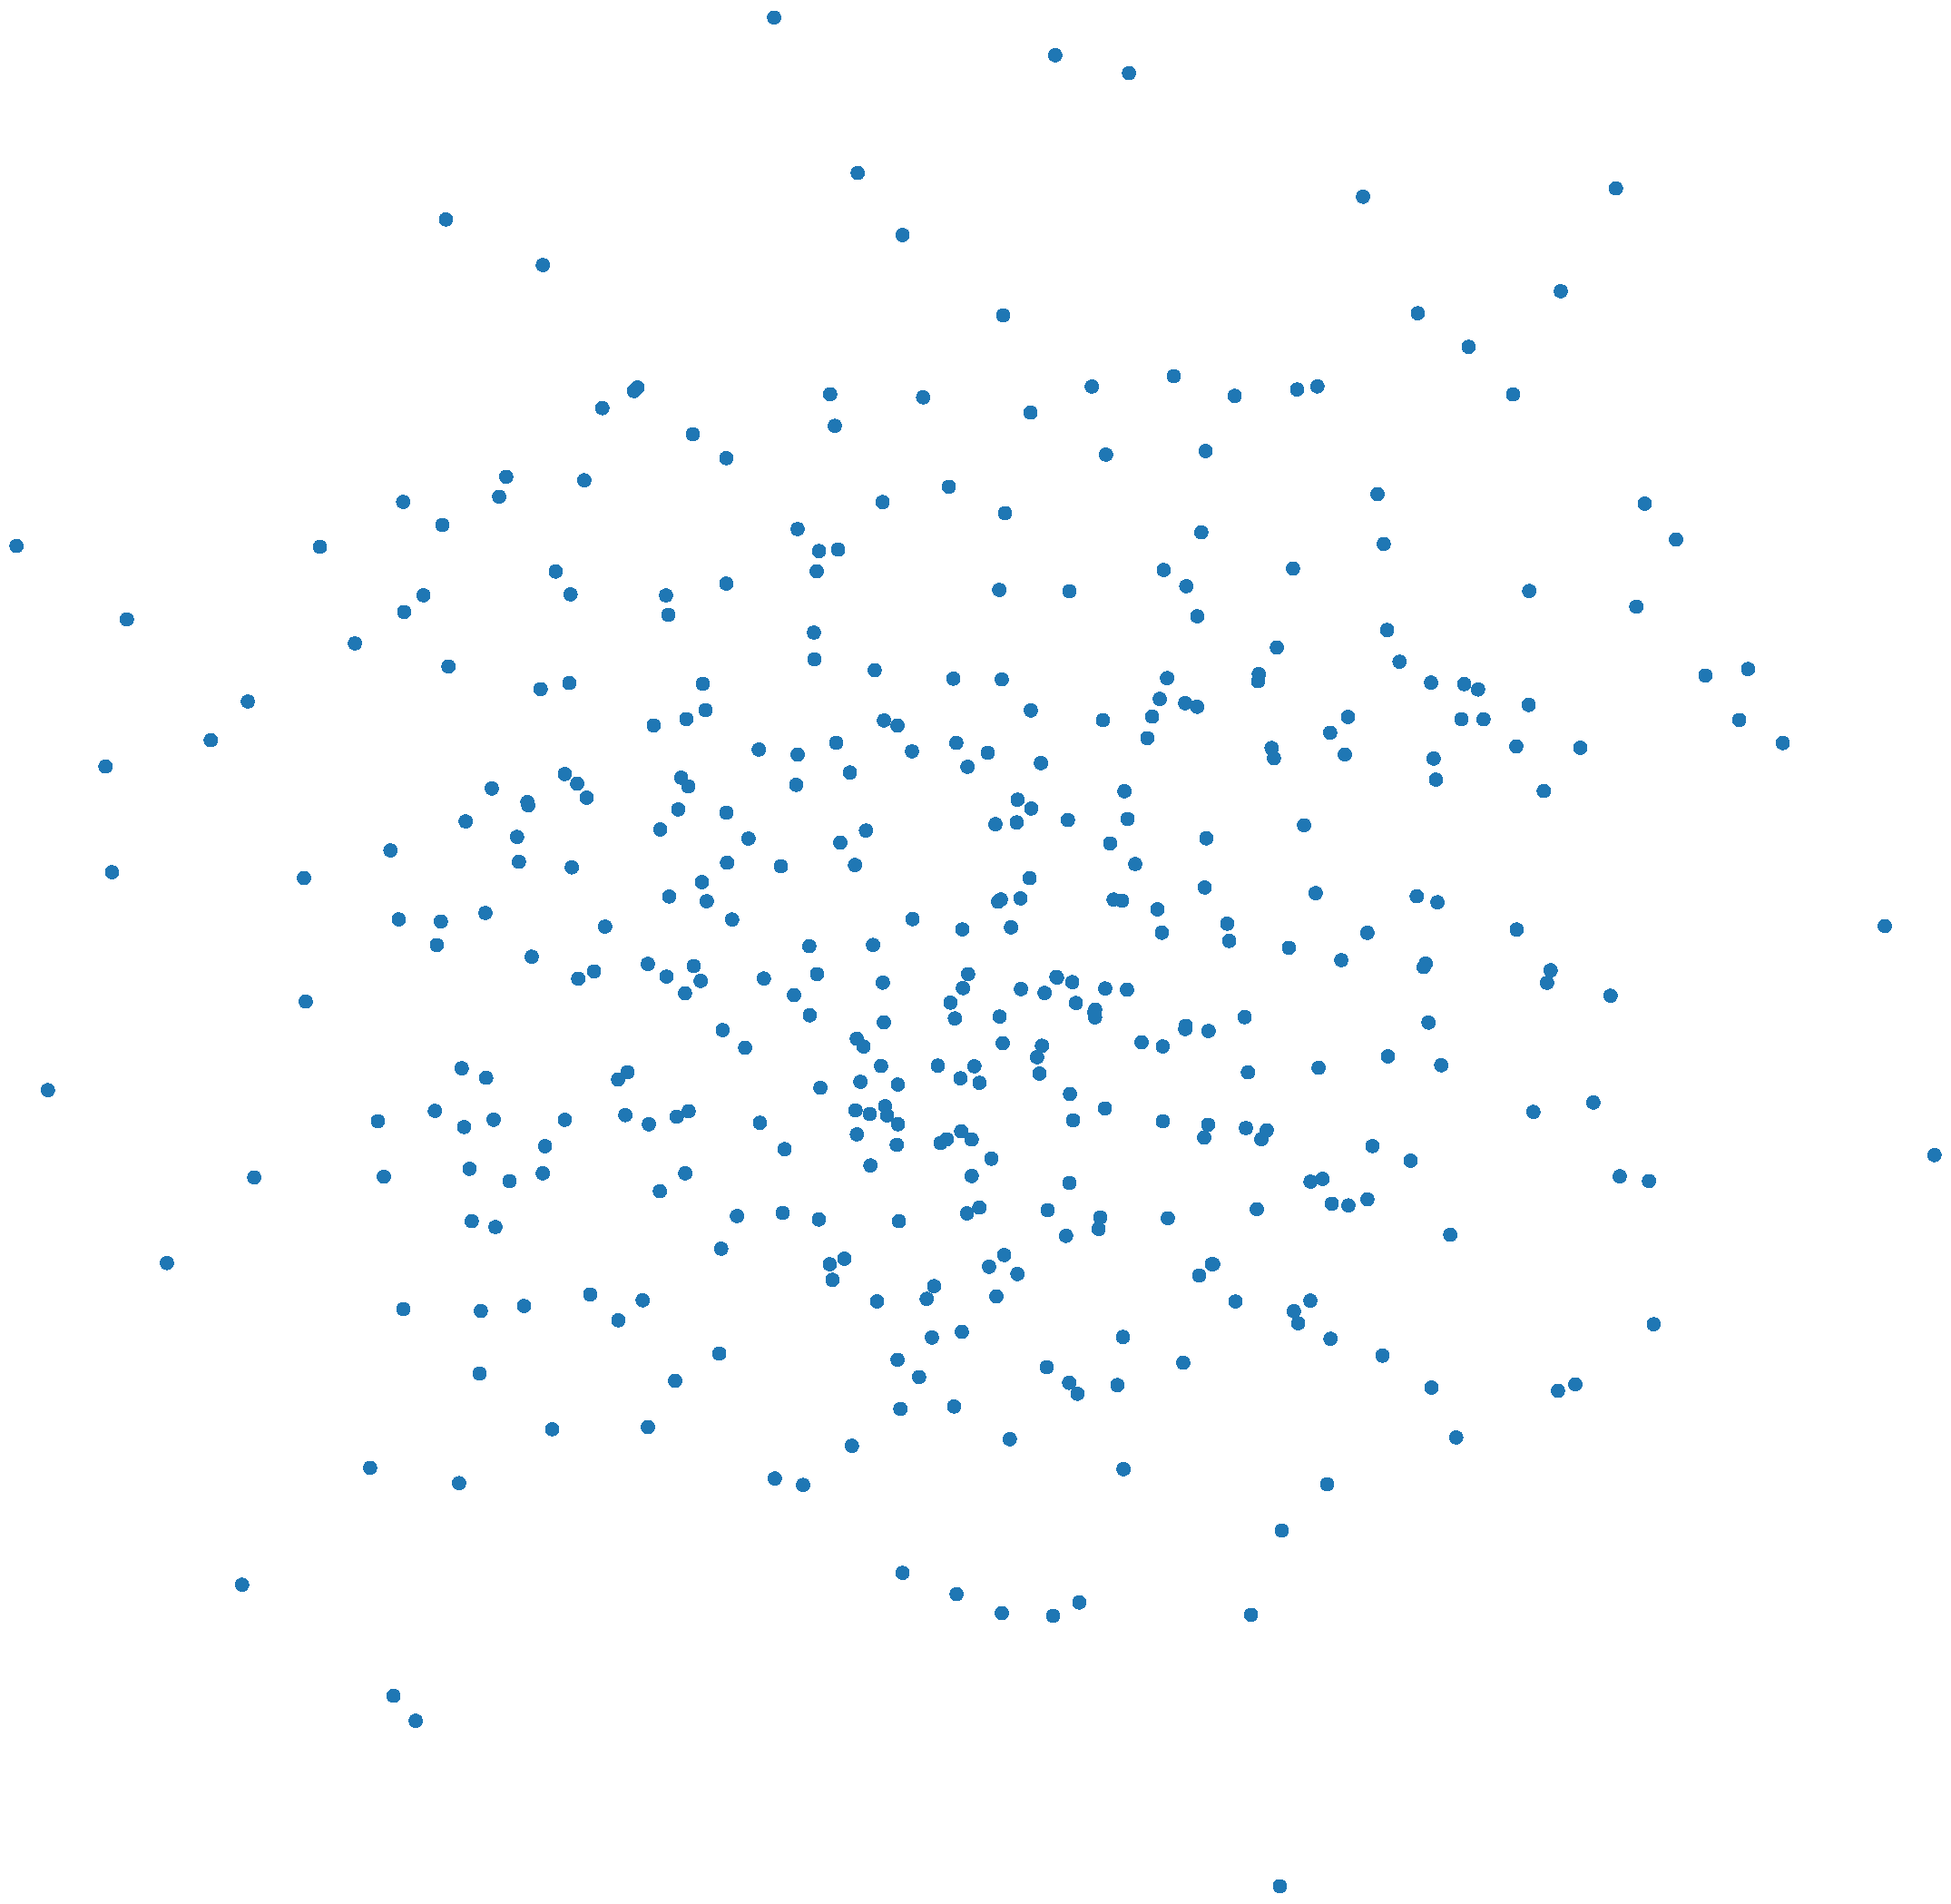
\includegraphics[width=.3\textwidth]{images/moon/zdist-crop.pdf}};
  \node[inner sep=0pt, right= 0.2cm of ffnn] (latentx) {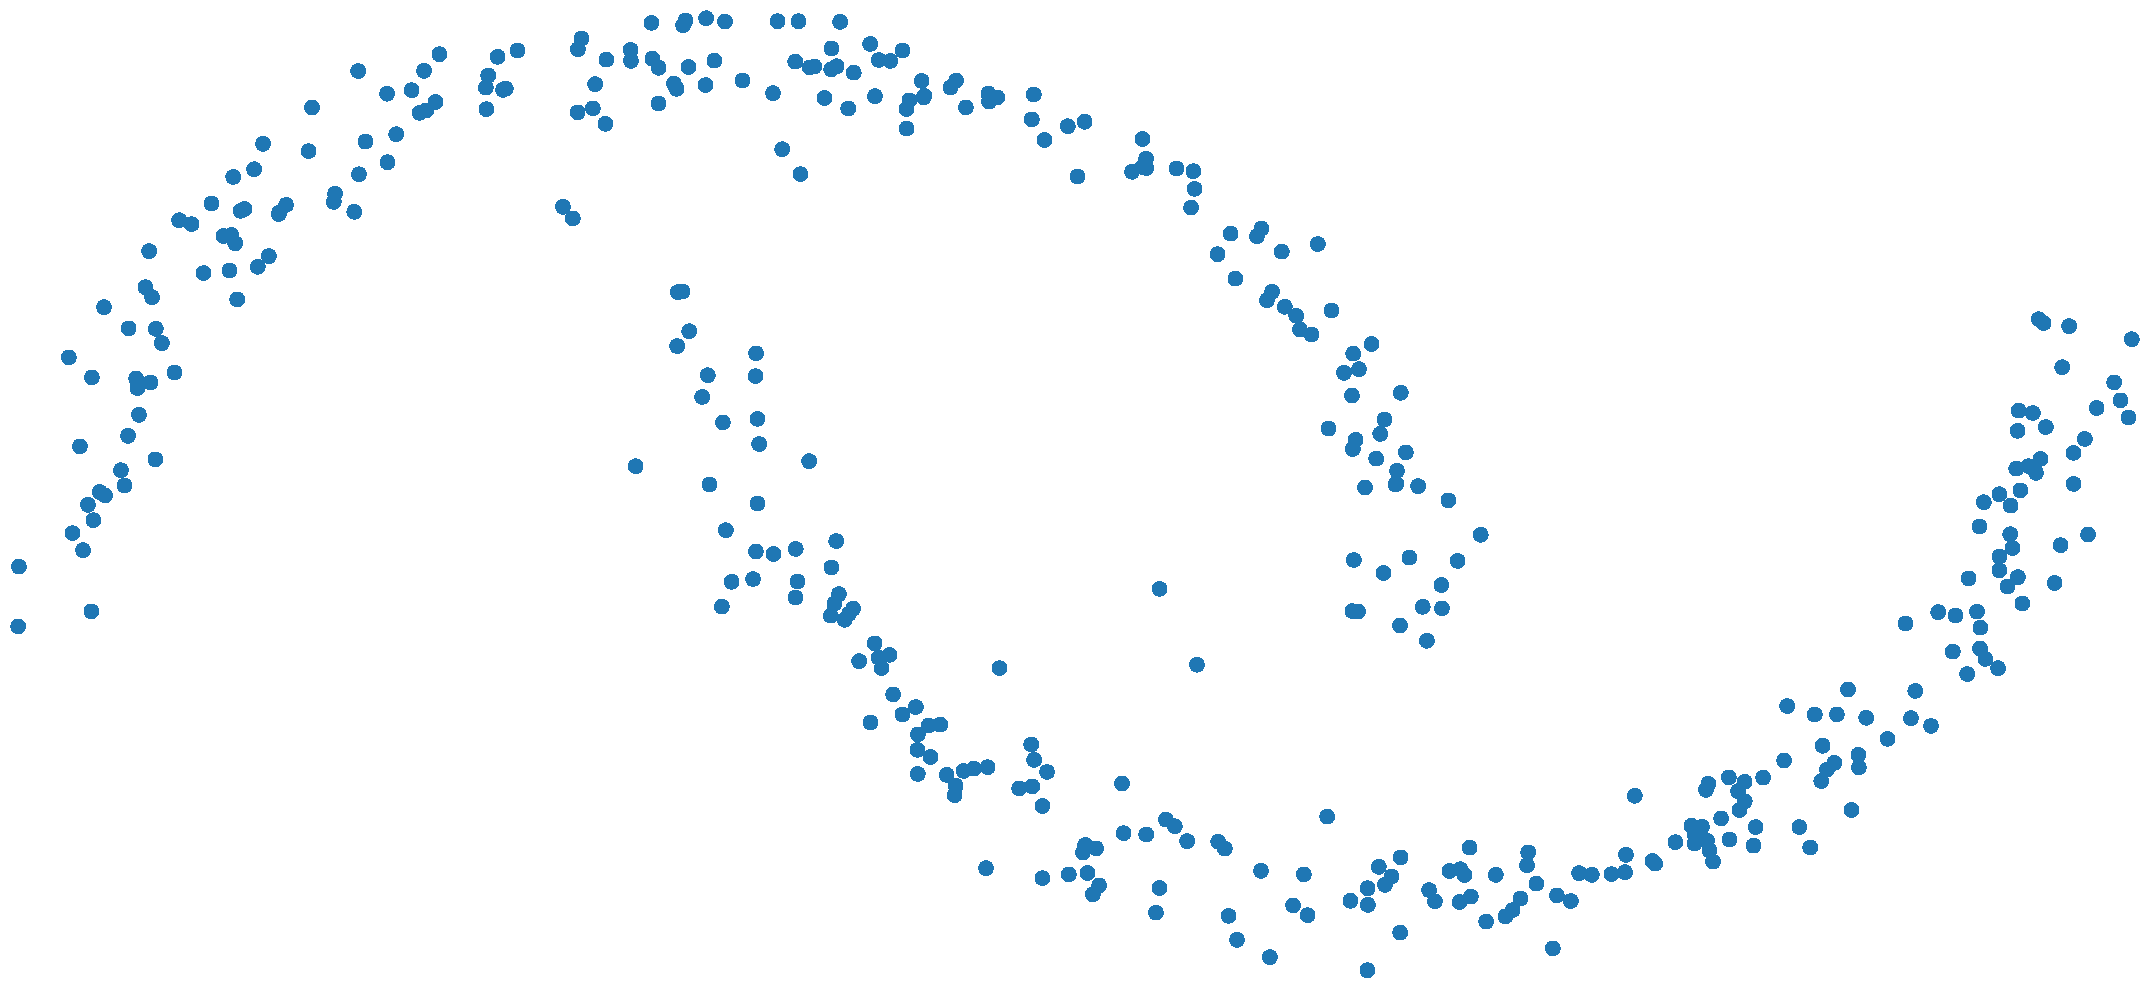
\includegraphics[width=.3\textwidth]{images/moon/xdist-crop.pdf}};
  
\end{scope}
%%% Local Variables:
%%% mode: latex
%%% TeX-master: "../ppgm_slide"
%%% End:

    \end{scope}
    \draw[dashed, ->, shorten >=5pt, shorten <=5pt, opacity=\bgopacity] ($(gk.north)+(0,0cm)$) -- ($(gk.north)+(0,-0.8cm)$);
    %%%%%%%%%%%%%%%%%%%%%%%%%%%%%%%%%%%%%%%% 
    %% 4. one layer mapping of the flow
    %%%%%%%%%%%%%%%%%%%%%%%%%%%%%%%%%%%%%%%% 
    
    \begin{scope}[shift={($(dgm.south)+(0,-1.5cm)$)}, scale=0.7, every node/.append style={transform shape}, local bounding box=oneLayer]
      % \tikzstyle{enode} = [thick, draw=blue, circle, inner sep = 3pt,
% align=center]
\tikzstyle{enode} = [thick, draw=black, circle, inner sep = 0, minimum size = 1cm,  align=center]
\tikzstyle{nnode} = [thick, rectangle, rounded corners = 2pt,minimum size = 0.4cm,draw,inner sep = 2pt]
\node[enode] (hal) at (-2,1) {$\bm{h}_{l,a}$};
\node[enode] (hbl) at (-2,-1) {$\bm{h}_{l,b}$};
\node[enode] (hal-1) at (2,1) {$\bm{h}_{l-1,a}$};
\node[enode] (hbl-1) at (2,-1) {$\bm{h}_{l-1,b}$};
\node[nnode] (times) at (-0.5,-1) {$\times$};
\node[nnode] (plus) at (0.5,-1) {$+$};
\node[nnode] (eq) at (0,1) {$=$};
\draw[->] (hal) -- node[fill=white] {$m_a$} (times);
\draw[->] (hal) -- node[fill=white] {$m_b$} (plus);
\draw[->] (hal) to (eq);

\draw[->] (eq) to (hal-1);
\draw[->] (hbl) to (times);
\draw[->] (times) to (plus);
\draw[->] (plus) to (hbl-1);
% \draw[draw=black] (-0.5,-0.5) rectangle ++(1,2);

%%% Local Variables:
%%% mode: latex
%%% TeX-master: "../ppgm_slide"
%%% End:

    \end{scope}
    \node [black, right=-0.5cm of oneLayer.east] {\scriptsize{Forward}};
    \node [black, below=1.3cm of oneLayer.west,anchor=west] (forwardmap) {
      \tiny
      \begin{minipage}{0.4\linewidth}
        \begin{equation*}
          \bm{h}_{l-1} =
          \begin{bmatrix}
            \bm{h}_{l-1,a}\\
            \bm{h}_{l-1,b}
          \end{bmatrix}
          =
          \begin{bmatrix}
            \bm{h}_{l,a}\\
            \bm{m}_a(\bm{h}_{l,a})\odot \bm{h}_{l,b} + \bm{m}_b(\bm{h}_{l,a})
          \end{bmatrix}
        \end{equation*}
      \end{minipage}
    };
    
    \begin{scope}[shift={($(oneLayer.south)+(0,-2.0cm)$)}, scale=0.7, every node/.append style={transform shape}, local bounding box=oneLayerInverse]
      % \tikzstyle{enode} = [thick, draw=blue, circle, inner sep = 3pt,
% align=center]
\tikzstyle{enode} = [thick, draw=blue, circle, inner sep = 0, minimum size = 1cm,  align=center]
\tikzstyle{nnode} = [thick, rectangle, rounded corners = 2pt,minimum size = 0.4cm,draw,inner sep = 2pt]
\node[enode] (hal) at (-2,1) {$\bm{h}_{l,a}$};
\node[enode] (hbl) at (-2,-1) {$\bm{h}_{l,b}$};
\node[enode] (hal-1) at (2,1) {$\bm{h}_{l-1,a}$};
\node[enode] (hbl-1) at (2,-1) {$\bm{h}_{l-1,b}$};
\node[nnode] (times) at (-0.5,-1) {$\div$};
\node[nnode] (plus) at (0.5,-1) {$-$};
\node[nnode] (eq) at (0,1) {$=$};
\draw[->] (hal-1) -- node[fill=white] {$\bm{m}_a$} (times);
\draw[->] (hal-1) -- node[fill=white] {$\bm{m}_b$} (plus);
\draw[<-] (hal) to (eq);

\draw[<-] (eq) to (hal-1);
\draw[->] (hbl) to (times);
\draw[<-] (times) to (plus);
\draw[<-] (plus) to (hbl-1);
% \draw[draw=black] (-0.5,-0.5) rectangle ++(1,2);


%%% Local Variables:
%%% mode: latex
%%% TeX-master: "../ppgm_slide"
%%% End:

    \end{scope}
    \node [black, right=-0.5cm of oneLayerInverse.east] {\scriptsize{Inverse}};

    \node [black, below=1.3cm of oneLayerInverse.west,anchor=west] (backwardmap) {
      \tiny
      \begin{minipage}{0.4\linewidth}
        \begin{equation*}
          \bm{h}_{l} =
          \begin{bmatrix}
            \bm{h}_{l,a}\\
            \bm{h}_{l,b}
          \end{bmatrix}
          =
          \begin{bmatrix}
            \bm{h}_{l-1,a}\\
            \left(  \bm{h}_{l-1,b} - \bm{m}_b(\bm{h}_{l-1,a}) \right)\oslash \bm{m}_a(\bm{h}_{l-1,a}) 
          \end{bmatrix}
        \end{equation*}
      \end{minipage}
    };

    \node [black, right=-0.5cm of oneLayerInverse.east] {\scriptsize{Inverse}};

    \node [black, right=2.3cm of oneLayerInverse.east,anchor=west] (attrtext) {
      \scriptsize
      \begin{minipage}{0.5\linewidth}
        \begin{itemize}[label=\textbullet]
        \item $\odot$ denotes element-wise product, $\oslash$ denotes
          element-wise division
        \item Mapping $\bm{m}_a$, $\bm{m}_b$ can be as complex as possible and not necessary invertible
        \item Same computation complexity of forward and inverse mapping
        \item Triangular matix of Jacobian
        \end{itemize}
        Alternative arch. on market: Auto-regressive flow, Glow, ODE, etc.
      \end{minipage}
    };
    \draw[green, ->] ($(oneLayer.east)+(3.5cm,0cm)$) --node [text width=5cm, black, right,above, anchor=north west]{\tiny Pick up one layer to zoom in} ($(oneLayer.east)+(1.1cm,0)$);
    
  \end{tikzpicture}
\end{frame}

\begin{frame}[label=current]{Remark}
  \begin{block}{On GenMM/GenHMM}
    free dimension to flexible model: number of mixture + complexity NNs;
    Compatible with statistic models and NN techniques;
    M-step, batch-gradient descent;
    duplicated NN for EM steps;
  \end{block}
\end{frame}

\begin{frame}[label=current]{Remark}
  \begin{block}{A diagram}
    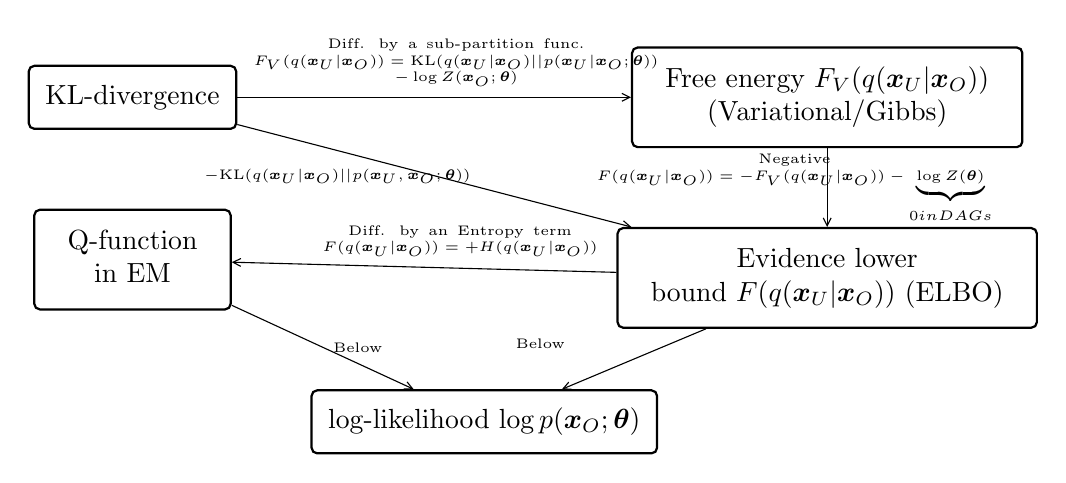
\begin{tikzpicture}
      \tikzstyle{cnode} = [thick, draw=black, circle, align=center, inner sep = 0.3pt]
      \tikzstyle{nnode} = [thick, rectangle, rounded corners = 2pt,minimum size = 0.8cm,draw,inner sep = 6pt]
      \node[nnode] (kl) at (0,0) {KL-divergence};
      \node[nnode, right= 5cm of kl] (freeEnergy) {\begin{tabular}{c}Free energy $F_V(q(\bm{x}_U|\bm{x}_O))$ \\ (Variational/Gibbs)\end{tabular}};
      \node[nnode, below= of freeEnergy] (elbo) {\begin{tabular}{c}Evidence lower\\ bound $F(q(\bm{x}_U|\bm{x}_O))$ (ELBO)\end{tabular}};
      \node[nnode, below= of kl] (q-fun) {\begin{tabular}{c}Q-function\\ in EM\end{tabular}};
      \node[nnode, below right= of q-fun] (llk) {log-likelihood $\log{p(\bm{x}_O;\bm{\theta})}$};
      \draw[black, ->] (kl) --node [text width=5cm, black, midway, above]{\tiny
        \begin{tabular}{c}
          Diff. by a sub-partition func. \\
          $F_V(q(\bm{x}_U|\bm{x}_O)) = \mathrm{KL}(q(\bm{x}_U|\bm{x}_O) || p(\bm{x}_U|\bm{x}_O; \bm{\theta})) $ \\
          $- \log{Z(\bm{x}_O; \bm{\theta})}$
        \end{tabular}}
      (freeEnergy);
      \draw[black, ->] (freeEnergy) --node [text width=3cm, black, midway, left]{\tiny
        \begin{tabular}{c}
          Negative \\
          $F(q(\bm{x}_U|\bm{x}_O)) = -F_V(q(\bm{x}_U|\bm{x}_O))- \underbrace{\log{Z(\bm{\theta})}}_{\text{0 in DAGs}}$
        \end{tabular}}
      (elbo);

      \draw[black, ->] (kl) --node [text width=3cm, black, midway, left]{\tiny
        \begin{tabular}{c}
          $-\mathrm{KL}(q(\bm{x}_U|\bm{x}_O) || p(\bm{x}_U,\bm{x}_O; \bm{\theta})) $
        \end{tabular}}
      (elbo);

      \draw[black, ->] (elbo) --node [text width=3cm, black, midway, above]{\tiny
        \begin{tabular}{c}
          Diff. by an Entropy term\\
          $F(q(\bm{x}_U|\bm{x}_O))= \Qq + H({q(\bm{x}_U|\bm{x}_O)})$
        \end{tabular}}
      (q-fun);

      \draw[black, ->] (elbo) --node [text width=3cm, black, midway, above]{\tiny
        Below
        }
      (llk);
      \draw[black, ->] (q-fun) --node [text width=3cm, black, midway, right]{\tiny
        Below
        }
      (llk);

      
    \end{tikzpicture}
  \end{block}
\end{frame}


%%% Local Variables:
%%% mode: latex
%%% TeX-master: "../ppgm_slide"
%%% End:

\subsection{EOT}
{ \setbeamercolor{background canvas}{bg=hl_bg}
  \setbeamercolor{normal text}{fg=hl_fg}
  \setbeamercolor{frametitle}{fg=hl_fg}
  \begin{frame}{What Have We been Talking About?}
    \usebeamercolor[fg]{normal text}
    
    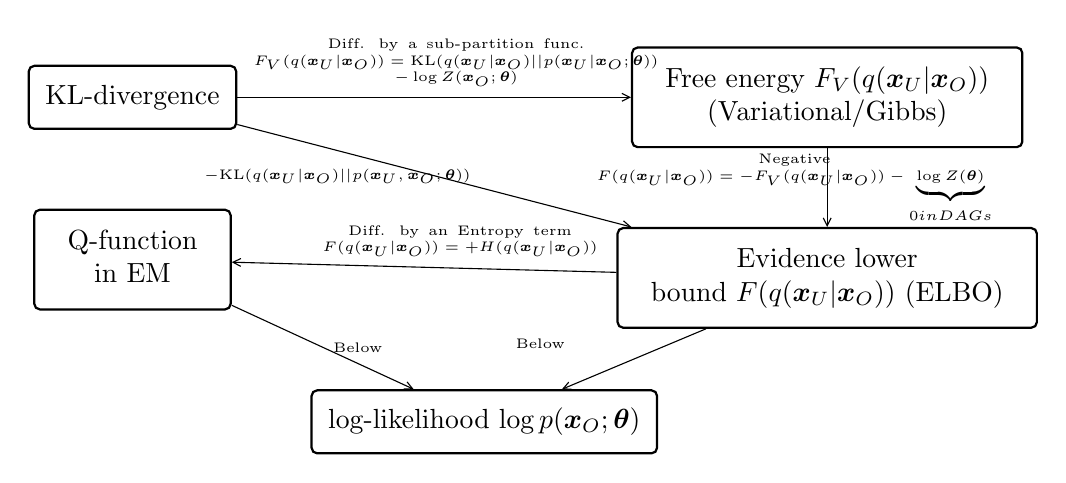
\begin{tikzpicture}
      \tikzstyle{cnode} = [thick, ellipse, align=center, draw, inner sep = 6pt]
      \tikzstyle{nnode} = [thick, rectangle, rounded corners = 2pt,minimum size = 0.8cm,draw,inner sep = 6pt]
      \node[nnode] (kl) at (0,0) {KL-divergence};
      \node[nnode, right= 5cm of kl] (freeEnergy) {\begin{tabular}{c}Free energy $F_V(q(\bm{x}_U|\bm{x}_O))$ \\ (Variational/Gibbs)\end{tabular}};
      \node[nnode, below= of freeEnergy] (elbo) {\begin{tabular}{c}Evidence lower\\ bound $F(q(\bm{x}_U|\bm{x}_O))$ (ELBO)\end{tabular}};
      \node[nnode, below= of kl] (q-fun) {\begin{tabular}{c}Q-function\\ in EM\end{tabular}};
      \node[nnode, below right= of q-fun] (llk) {log-likelihood $\log{p(\bm{x}_O;\bm{\theta})}$};
      \draw[black, ->] (kl) --node [text width=5cm, black, midway, above]{\tiny
        \begin{tabular}{c}
          Diff. by a sub-partition func. \\
          $F_V(q(\bm{x}_U|\bm{x}_O)) = \mathrm{KL}(q(\bm{x}_U|\bm{x}_O) || p(\bm{x}_U|\bm{x}_O; \bm{\theta})) $ \\
          $- \log{Z(\bm{x}_O; \bm{\theta})}$
        \end{tabular}}
      (freeEnergy);
      \draw[black, ->] (freeEnergy) --node [text width=3cm, black, midway, left]{\tiny
        \begin{tabular}{c}
          Negative \\
          $F(q(\bm{x}_U|\bm{x}_O)) = -F_V(q(\bm{x}_U|\bm{x}_O))- \underbrace{\log{Z(\bm{\theta})}}_{\text{0 in DAGs}}$
        \end{tabular}}
      (elbo);

      \draw[black, ->] (kl) --node [text width=3cm, black, midway, left]{\tiny
        \begin{tabular}{c}
          $-\mathrm{KL}(q(\bm{x}_U|\bm{x}_O) || p(\bm{x}_U,\bm{x}_O; \bm{\theta})) $
        \end{tabular}}
      (elbo);

      \draw[black, ->] (elbo) --node [text width=3cm, black, midway, above]{\tiny
        \begin{tabular}{c}
          Diff. by an Entropy term\\
          $F(q(\bm{x}_U|\bm{x}_O))= \Qq + H({q(\bm{x}_U|\bm{x}_O)})$
        \end{tabular}}
      (q-fun);

      \draw[black, ->] (elbo) --node [text width=3cm, black, midway, above]{\tiny
        Below
      }
      (llk);
      \draw[black, ->] (q-fun) --node [text width=3cm, black, midway, right]{\tiny
        Below
      }
      (llk);
      
    \end{tikzpicture}
    \only<2->{
      \begin{textblock}{5}(6,6)
        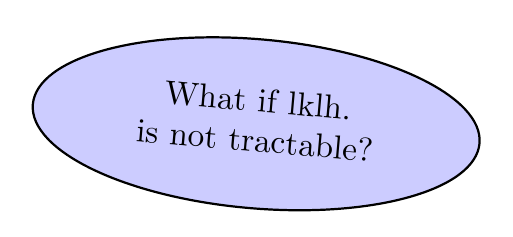
\begin{tikzpicture}[scale=1.2,auto,rotate=-5,transform shape]
          \tikzstyle{cnode} = [fill=blue!20,thick, ellipse, align=center, draw, inner sep = 6pt]
          \node [cnode, text=black] (question) at (0, 0) {\begin{tabular}{c}What if lklh. \\is not tractable?\end{tabular}};
          
        \end{tikzpicture}
      \end{textblock}
    }
    % \let\thefootnote\relax\footnotetext{\tiny
    % \vskip -0.2cm
    % A bit notation abuse, $\bm{x}_U$ corresponds to unobserved variable $\bm{z}$.
    % }
    
  \end{frame}
}

{ \setbeamercolor{background canvas}{bg=hl_bg}
  \setbeamercolor{normal text}{fg=hl_fg}
  \setbeamercolor{frametitle}{fg=hl_fg}
  \begin{frame}[label=current]
    \usebeamercolor[fg]{normal text}
    \begin{center}
      {
        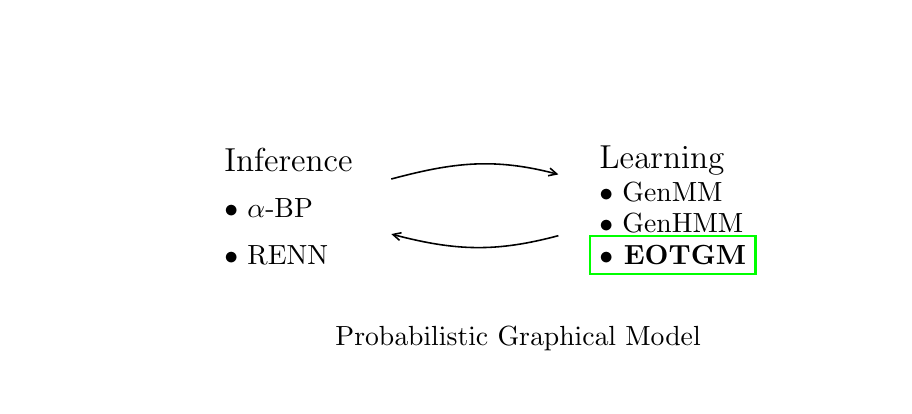
\begin{tikzpicture}
          \tikzstyle{cnode} = [thick, draw=white, ellipse, inner sep = 2pt,  align=center]
          \tikzstyle{fnode} = [thick, draw=white, ellipse, inner sep = 10pt,  align=center]
          \tikzstyle{rnode} = [thick, rectangle, inner sep = 1.5pt,  align=left]
          \node[rnode] (inf) at (-2, 0) {\large Inference};
          \node[rnode, below = 0.6cm of inf.west, anchor=west] (abp) {$\bullet$ {$\alpha$-BP}};
          \node[rnode, below = 1.2cm of inf.west, anchor=west] (renn) {$\bullet$ RENN};
          \node[cnode, fit=(abp)(inf)(renn)] (infn) {};
          
          \node[rnode, right = 3 of inf] (lern) {\large Learning};
          \node[rnode, below = 0.4 of lern.west, anchor=west] (genmm) {$\bullet$ GenMM};
          \node[rnode, below = 0.8 of lern.west, anchor=west] (genhmm) {{$\bullet$} GenHMM};
          \node[rnode, below = 1.2 of lern.west, anchor=west] (lfree) {\textbf{{$\bullet$} EOTGM}};
          \node[cnode, fit=(lern)(genmm)(genhmm)(lfree)] (learn) {};
          \node[rnode, draw=green, fit=(lfree)] () {};

          \node[fnode, fit=(infn)(lern)] (box) {};

          
          \node[below right = 0.5 and -0.5 of infn] {{Probabilistic} Graphical Model};
          \draw[->,line width=0.2mm] (infn) to[out=15, in=165] (learn);
          \draw[->,line width=0.2mm] (learn) to[out=195, in=-15] (infn);
        \end{tikzpicture}
      }
    \end{center}
    
  \end{frame}
}

\begin{frame}[label=current]{Where is the learning info. from?}
  \begin{tikzpicture}
    \tikzstyle{enode} = [thick, draw, circle, inner sep = 4pt,  align=center]
    \tikzstyle{elnode} = [thick, draw, ellipse, inner sep = 1pt,  align=center]
    \tikzstyle{nnode} = [thick, rectangle, rounded corners = 2pt,draw,inner sep = 4pt]
    \node[enode] (z) at (-4,0) {$\bm{Z}$};
    \node[enode, right=2cm of z] (x) {$\bm{X}$};
    \node[elnode] (emp) [right= 6.5cm of x] {Empirical \\samples};
    
    \draw[->] (z) -- node[nnode,fill=white] {$\bm{g}$} (x);
    \draw[<->] (x) -- node[draw, rounded corners = 2pt, fill=blue!30, align=center] (trckmetric) {
      \begin{minipage}{0.45\textwidth}
        How different they are
        \begin{itemize}[label=\textbullet]
        \item likelihood
        \item Evidence lower bound, free energy 
        \item KL-divergence, $\alpha$-divergence
        \end{itemize}
      \end{minipage}} (emp);
    \node[fill=white!30, below= of trckmetric, align=center] (ot) {
      \begin{minipage}{0.6\textwidth}
        Optimal transport (OT): moving mass from a dist. to another
        \begin{equation*}
          T(p^{\ast},p)=\min_{ \pi \in \Pi(p^{\ast},p)} \dotp{\underbrace{\pi}_{\text{marginalize to $p^{\ast},p$}}}{\underbrace{\bm{M}}_{\text{\begin{tabular}{c}cost matrix\\ sample difference \end{tabular}}}},
        \end{equation*}
        Key attributes:
        \begin{itemize}[label=\textbullet]
        \item Doesnot require tractible lklh.
        \item Learning gradient info. from sample comparison
        \item High complexity, each evaluation is sovling an optimization problem
        \end{itemize}
      \end{minipage}
    };
    \draw[->] (trckmetric) -- node[black, midway, right] {add-on} (ot);

  \end{tikzpicture}
  \only<2>{
    \begin{textblock}{5}(2,4.3)
      \begin{tikzpicture}
        \node[rounded corners = 4pt, rectangle, inner sep = 4pt, fill=gray!20, align=center, text width=10cm, label=below:{A toy example}] (ot_kl) at (0,0)
        {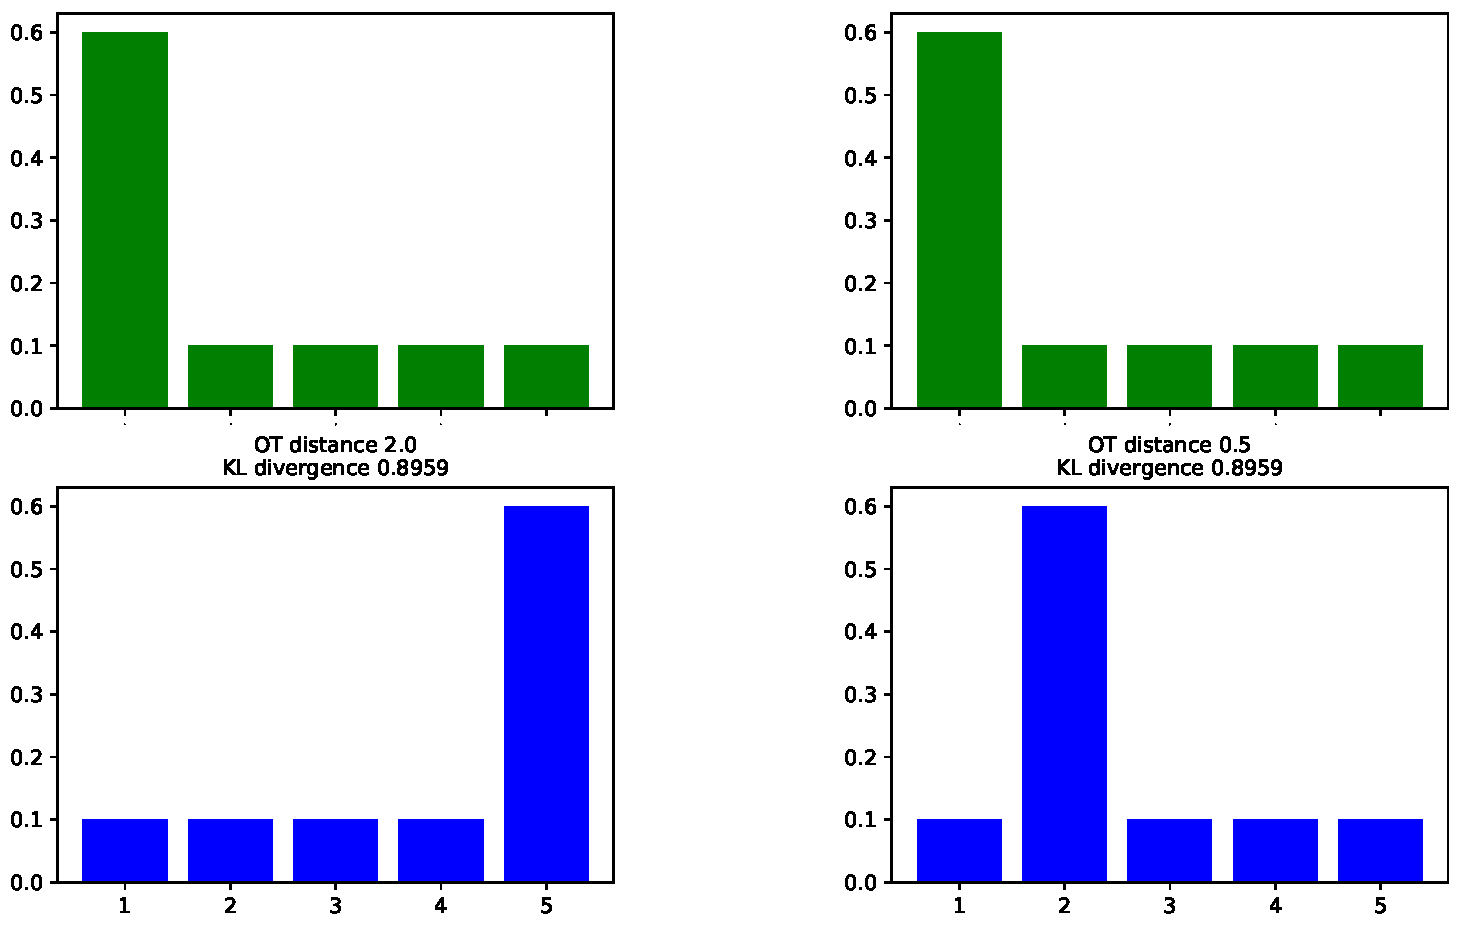
\includegraphics[width=1\linewidth]{images/ot_kl.pdf}};
      \end{tikzpicture}
    \end{textblock}
  }
\end{frame}


\begin{frame}[label=current]{EOTGM Explained}
  \begin{tikzpicture}
    \tikzstyle{enode}=[thick, draw, circle, inner sep = 8pt,  align=center]
    \tikzstyle{elnode}=[thick, draw, rectangle, rounded corners = 2pt, inner sep = 4pt, align=center]
    \tikzstyle{nnode} = [thick, rectangle, rounded corners = 2pt,minimum size = 4.8cm,draw,inner sep = 2pt]
    \node[elnode] (ot) at (-1,0) {OT $\min\;T(p^{\ast},p)$};
    % \node[nnode] at (0,1) {$T(P,Q) = \min_{\Gamma\in\Pp(P,Q) }\EE_{(X,Y)\sim \Gamma}\left[ c(X,Y) \right]$};
    \node[elnode] (wgan) at (6,0) {\begin{tabular}{c}WGAN, Arjovsky, et al\\ {\tiny Wasserstein Generative Adversarial Network} \\ {\tiny An adversarial game} \\ {\tiny \textit{1-Lipschitz function family}}\end{tabular}};
    \node[elnode] (eot) at (3,-2) {\begin{tabular}{c} EOTGM \\ {\tiny NN generator + Sinkhorn solver} \\ {\tiny Applicable to implicit \& explicit models} \end{tabular}};
    \draw[->] (ot) -- node[midway,above] {\tiny Kantorovich duality} (wgan);
    \draw[->] (ot) -- node[midway,right] {\tiny Entropy regularization} (eot);
    \node[text width=4cm] [right=-0.1cm of eot] {\begin{equation*} \min_{p} \underbrace{\min_{\pi\in\Pp(p^{\ast},p) } \dotp{\pi}{\bm{M}} - \la H(\pi)}_{W(p^{\ast}, p)}
      \end{equation*}};   
  \end{tikzpicture}
  Alternatively scale the rows \& columns of matrix $e^{-\bm{M}/\lambda}$ (Sinkhorn) gives 'soft' solution
  \begin{itemize}[label=\textbullet]
  \item joint distribution $\pi^{\ast}$
  \item subgradient $\beta^{\ast}$
  \end{itemize}
  which provides the gradient information for adjusting $\bm{g}$.
  \only<2>{
    \begin{textblock}{5}(2,4.3)
      \begin{tikzpicture}
        
        \begin{scope}[scale=1.6, local bounding box=algo]
          % Graphic for TeX using PGF
% Title: /home/dong/Documents/phd_research/my_papers/entropy-wgan/poster/figs/alo_flow.dia
% Creator: Dia v0.97.3
% CreationDate: Wed Apr 24 18:01:40 2019
% For: dong
% \usepackage{tikz}
% The following commands are not supported in PSTricks at present
% We define them conditionally, so when they are implemented,
% this pgf file will use them.
\ifx\du\undefined
  \newlength{\du}
\fi
\setlength{\du}{5\unitlength}
\pgftransformxscale{1.000000}
\pgftransformyscale{-1.000000}
\definecolor{dialinecolor}{rgb}{0.000000, 0.000000, 0.000000}
\pgfsetstrokecolor{dialinecolor}
\definecolor{dialinecolor}{rgb}{1.000000, 1.000000, 1.000000}
\pgfsetfillcolor{dialinecolor}
\pgfsetlinewidth{0.100000\du}
\pgfsetdash{}{0pt}
\pgfsetdash{}{0pt}
\pgfsetbuttcap
{
\definecolor{dialinecolor}{rgb}{0.000000, 0.000000, 0.000000}
\pgfsetfillcolor{dialinecolor}
% was here!!!
\definecolor{dialinecolor}{rgb}{0.000000, 0.000000, 0.000000}
\pgfsetstrokecolor{dialinecolor}
\draw (18.524007\du,0.865483\du)--(18.528518\du,3.644891\du);
}
\pgfsetlinewidth{0.100000\du}
\pgfsetdash{}{0pt}
\pgfsetdash{}{0pt}
\pgfsetbuttcap
{
\definecolor{dialinecolor}{rgb}{0.000000, 0.000000, 0.000000}
\pgfsetfillcolor{dialinecolor}
% was here!!!
\definecolor{dialinecolor}{rgb}{0.000000, 0.000000, 0.000000}
\pgfsetstrokecolor{dialinecolor}
\draw (18.500105\du,3.590367\du)--(27.515393\du,3.588352\du);
}
\pgfsetlinewidth{0.100000\du}
\pgfsetdash{}{0pt}
\pgfsetdash{}{0pt}
\pgfsetbuttcap
{
\definecolor{dialinecolor}{rgb}{0.000000, 0.000000, 0.000000}
\pgfsetfillcolor{dialinecolor}
% was here!!!
\definecolor{dialinecolor}{rgb}{0.000000, 0.000000, 0.000000}
\pgfsetstrokecolor{dialinecolor}
\draw (9.531143\du,3.591676\du)--(18.546431\du,3.589661\du);
}
\pgfsetlinewidth{0.100000\du}
\pgfsetdash{}{0pt}
\pgfsetdash{}{0pt}
\pgfsetbuttcap
{
\definecolor{dialinecolor}{rgb}{0.000000, 0.000000, 0.000000}
\pgfsetfillcolor{dialinecolor}
% was here!!!
\pgfsetarrowsend{latex}
\definecolor{dialinecolor}{rgb}{0.000000, 0.000000, 0.000000}
\pgfsetstrokecolor{dialinecolor}
\draw (9.554590\du,3.555355\du)--(9.545014\du,6.552207\du);
}
\pgfsetlinewidth{0.100000\du}
\pgfsetdash{}{0pt}
\pgfsetdash{}{0pt}formu
\pgfsetbuttcap
{
\definecolor{dialinecolor}{rgb}{0.000000, 0.000000, 0.000000}
\pgfsetfillcolor{dialinecolor}
% was here!!!
\pgfsetarrowsend{latex}
\definecolor{dialinecolor}{rgb}{0.000000, 0.000000, 0.000000}
\pgfsetstrokecolor{dialinecolor}
\draw (27.515539\du,3.579062\du)--(27.518490\du,6.615272\du);
}
% setfont left to latex
\definecolor{dialinecolor}{rgb}{0.000000, 0.000000, 0.000000}
\pgfsetstrokecolor{dialinecolor}
\node[anchor=west] at (18.801352\du,2.255187\du){\tiny Explicity model?};
% setfont left to latex
\definecolor{dialinecolor}{rgb}{0.000000, 0.000000, 0.000000}
\pgfsetstrokecolor{dialinecolor}
\node[anchor=west] at (12.404325\du,3.043961\du){Yes};
% setfont left to latex
\definecolor{dialinecolor}{rgb}{0.000000, 0.000000, 0.000000}
\pgfsetstrokecolor{dialinecolor}
\node[anchor=west] at (25.516919\du,3.045657\du){No};
\pgfsetlinewidth{0.100000\du}
\pgfsetdash{}{0pt}
\pgfsetdash{}{0pt}
\pgfsetmiterjoin
\definecolor{dialinecolor}{rgb}{0.000000, 0.000000, 0.000000}
\pgfsetstrokecolor{dialinecolor}
\draw (6.132662\du,6.958798\du)--(6.132662\du,13.481742\du)--(17.882368\du,13.481742\du)--(17.882368\du,6.958798\du)--cycle;
\pgfsetlinewidth{0.100000\du}
\pgfsetdash{}{0pt}
\pgfsetdash{}{0pt}
\pgfsetmiterjoin
\definecolor{dialinecolor}{rgb}{0.000000, 0.000000, 0.000000}
\pgfsetstrokecolor{dialinecolor}
\draw (18.629924\du,6.913963\du)--(18.629924\du,13.436908\du)--(30.379629\du,13.436908\du)--(30.379629\du,6.913963\du)--cycle;
% setfont left to latex
\definecolor{dialinecolor}{rgb}{0.000000, 0.000000, 0.000000}
\pgfsetstrokecolor{dialinecolor}
\node[anchor=west] at (5.856351\du,10.251070\du){\tiny {\vbox{
  \begin{itemize}[label=\textbullet]
  \item Gradient chain rule
  \item Direct optimization
    \item[] w.r.t. model parameters
  \end{itemize}}}};
% setfont left to atex
\definecolor{dialinecolor}{rgb}{0.000000, 0.000000, 0.000000}
\pgfsetstrokecolor{dialinecolor}
\node[anchor=west] at (18.52029\du,10.254778\du){\tiny {\vbox{
      \begin{itemize}[label=\textbullet]
        \item Richer choice of $\bm{g}$
  \item Formulate loss by $\pi^{\ast}_{\lambda}$
  \item Error back-propagation
    \item[] by auto gradient tools
  \end{itemize}}}};
\pgfsetlinewidth{0.100000\du}
\pgfsetdash{}{0pt}
\pgfsetdash{}{0pt}
\pgfsetbuttcap
\pgfsetmiterjoin
\pgfsetlinewidth{0.100000\du}
\pgfsetbuttcap
\pgfsetmiterjoin
\pgfsetdash{}{0pt}
\definecolor{dialinecolor}{rgb}{0.000000, 0.000000, 0.000000}
\pgfsetstrokecolor{dialinecolor}
\draw (15.723295\du,-3.076184\du)--(16.205111\du,-6.930706\du)--(20.541447\du,-8.857967\du)--(24.877784\du,-6.930706\du)--(25.359599\du,-3.076184\du)--(22.950523\du,0.296522\du)--(18.132371\du,0.296522\du)--cycle;
\pgfsetlinewidth{0.010000\du}
\pgfsetbuttcap
\pgfsetmiterjoin
\pgfsetdash{}{0pt}
\definecolor{dialinecolor}{rgb}{0.000000, 0.000000, 0.000000}
\pgfsetstrokecolor{dialinecolor}
\draw (15.723295\du,-3.076184\du)--(16.205111\du,-6.930706\du)--(20.541447\du,-8.857967\du)--(24.877784\du,-6.930706\du)--(25.359599\du,-3.076184\du)--(22.950523\du,0.296522\du)--(18.132371\du,0.296522\du)--cycle;
\pgfsetlinewidth{0.100000\du}
\pgfsetdash{}{0pt}
\pgfsetdash{}{0pt}
\pgfsetbuttcap
{
\definecolor{dialinecolor}{rgb}{0.000000, 0.000000, 0.000000}
\pgfsetfillcolor{dialinecolor}
% was here!!!
\pgfsetarrowsstart{latex}
\definecolor{dialinecolor}{rgb}{0.000000, 0.000000, 0.000000}
\pgfsetstrokecolor{dialinecolor}
\draw (14.704266\du,-9.125968\du)--(10.750000\du,-0.302492\du);
}
\pgfsetlinewidth{0.100000\du}
\pgfsetdash{}{0pt}
\pgfsetdash{}{0pt}
\pgfsetmiterjoin
\pgfsetbuttcap
{
\definecolor{dialinecolor}{rgb}{0.000000, 0.000000, 0.000000}
\pgfsetfillcolor{dialinecolor}
% was here!!!
\pgfsetarrowsstart{latex}
\definecolor{dialinecolor}{rgb}{0.000000, 0.000000, 0.000000}
\pgfsetstrokecolor{dialinecolor}
\pgfpathmoveto{\pgfpoint{18.132371\du}{0.296522\du}}
\pgfpathcurveto{\pgfpoint{18.682371\du}{-2.653478\du}}{\pgfpoint{20.600968\du}{-2.060704\du}}{\pgfpoint{21.200968\du}{-4.360704\du}}
\pgfusepath{stroke}
}
\pgfsetlinewidth{0.100000\du}
\pgfsetdash{{1.000000\du}{1.000000\du}}{0\du}
\pgfsetdash{{1.000000\du}{1.000000\du}}{0\du}
\pgfsetbuttcap
{
\definecolor{dialinecolor}{rgb}{0.000000, 0.000000, 0.000000}
\pgfsetfillcolor{dialinecolor}
% was here!!!
\definecolor{dialinecolor}{rgb}{0.000000, 0.000000, 0.000000}
\pgfsetstrokecolor{dialinecolor}
\draw (11.839663\du,-2.816111\du)--(18.080386\du,0.347759\du);
}
\pgfsetlinewidth{0.100000\du}
\pgfsetdash{}{0pt}
\pgfsetdash{}{0pt}
\pgfsetbuttcap
{
\definecolor{dialinecolor}{rgb}{0.000000, 0.000000, 0.000000}
\pgfsetfillcolor{dialinecolor}
% was here!!!
\definecolor{dialinecolor}{rgb}{0.000000, 0.000000, 0.000000}
\pgfsetstrokecolor{dialinecolor}
\draw (12.356671\du,-2.597719\du)--(12.670233\du,-3.241992\du);
}
\pgfsetlinewidth{0.100000\du}
\pgfsetdash{}{0pt}
\pgfsetdash{}{0pt}
\pgfsetbuttcap
{
\definecolor{dialinecolor}{rgb}{0.000000, 0.000000, 0.000000}
\pgfsetfillcolor{dialinecolor}
% was here!!!
\definecolor{dialinecolor}{rgb}{0.000000, 0.000000, 0.000000}
\pgfsetstrokecolor{dialinecolor}
\draw (12.676482\du,-3.210742\du)--(12.096348\du,-3.498168\du);
}
% setfont left to latex
\definecolor{dialinecolor}{rgb}{0.000000, 0.000000, 0.000000}
\pgfsetstrokecolor{dialinecolor}
\node[anchor=west] at (18.030166\du,-5.041491\du){$p^{\ast}\cdot p^{\intercal}$, $\lambda \rightarrow \infty$};
% setfont left to latex
\definecolor{dialinecolor}{rgb}{0.000000, 0.000000, 0.000000}
\pgfsetstrokecolor{dialinecolor}
\node[anchor=west] at (12.022945\du,-7.745138\du){$\pd{W}{\theta}$};
\pgfsetlinewidth{0.100000\du}
\pgfsetdash{}{0pt}
\pgfsetdash{}{0pt}
\pgfsetbuttcap
\pgfsetmiterjoin
\pgfsetlinewidth{0.100000\du}
\pgfsetbuttcap
\pgfsetmiterjoin
\pgfsetdash{}{0pt}
\definecolor{dialinecolor}{rgb}{0.000000, 0.000000, 0.000000}
\pgfsetfillcolor{dialinecolor}
\pgfpathellipse{\pgfpoint{18.464159\du}{-1.026639\du}}{\pgfpoint{0.159762\du}{0\du}}{\pgfpoint{0\du}{0.159762\du}}
\pgfusepath{fill}
\definecolor{dialinecolor}{rgb}{0.000000, 0.000000, 0.000000}
\pgfsetstrokecolor{dialinecolor}
\pgfpathellipse{\pgfpoint{18.464159\du}{-1.026639\du}}{\pgfpoint{0.159762\du}{0\du}}{\pgfpoint{0\du}{0.159762\du}}
\pgfusepath{stroke}
\pgfsetbuttcap
\pgfsetmiterjoin
\pgfsetdash{}{0pt}
\definecolor{dialinecolor}{rgb}{0.000000, 0.000000, 0.000000}
\pgfsetstrokecolor{dialinecolor}
\pgfpathellipse{\pgfpoint{18.464159\du}{-1.026639\du}}{\pgfpoint{0.159762\du}{0\du}}{\pgfpoint{0\du}{0.159762\du}}
\pgfusepath{stroke}
% setfont left to latex
\definecolor{dialinecolor}{rgb}{0.000000, 0.000000, 0.000000}
\pgfsetstrokecolor{dialinecolor}
\node[anchor=west] at (18.985501\du,-0.965533\du){$\pi^{\ast}_{\lambda}$};



        \end{scope}
        \begin{scope}[on background layer]
          \node[rounded corners = 4pt, rectangle, inner sep = 4pt, fill=gray!20, align=center, text width=10cm, label=below:{}, fit=(algo)] () {};
        \end{scope}
        
      \end{tikzpicture}
    \end{textblock}
  }

  \let\thefootnote\relax\footnotetext{\tiny
    Marco Cuturi. Sinkhorn distances: Lightspeed computation of optimal transport}
\end{frame}

\begin{frame}[label=current]{EOTGM and EOTGAN}
  EOTGM\\
  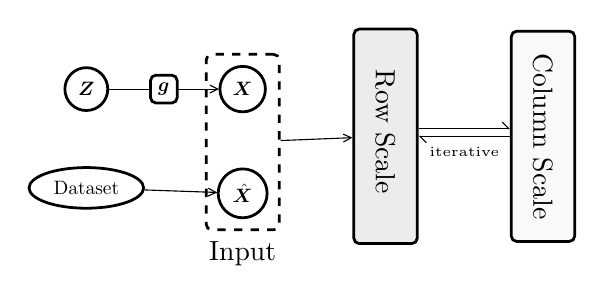
\begin{tikzpicture}
    \tikzstyle{enode} = [draw, circle, inner sep = 4pt,  align=center]
    \tikzstyle{nnode} = [rectangle, rounded corners = 2pt,draw,inner sep = 4pt]
    \tikzstyle{ecnode} = [draw, ellipse, inner sep = 4pt,  align=center]

    \begin{scope}[scale=0.7, every node/.append style={transform shape}]
      \node[enode] (z) at (-4,0) {$\bm{Z}$};
      \node[enode, right=2cm of z] (x) {$\bm{X}$};
      \node[enode, below= of x] (hx) {$\hat{\bm{X}}$};
      \node[ecnode, below= of z] (data) {Dataset};

      \draw[->] (z) -- node[nnode,fill=white] {$\bm{g}$} (x);
      \draw[->] (data) -- (hx);
    \end{scope}
    \node[nnode,fit=(x)(hx), label={below:{Input}}, dashed] (inPair) {};
    
    \node[nnode, rotate=-90, inner sep = 8pt, fill=gray!15] (rowScale) at (1,-0.6) {~~Row Scale~~~~};
    \node[nnode, rotate=-90, inner sep = 8pt, fill=gray!5] (colScale) at (3,-0.6) {Column Scale};

    \draw[->] (inPair) to (rowScale);
    \draw [-{Straight Barb[left]}] ($(rowScale.north) + (0, 0.1) $) to ($(colScale.south) +(0,0.1)$);
    \draw [-{Straight Barb[left]}] (colScale) -- node[black, midway, below] {\tiny iterative} (rowScale) ;
    
  \end{tikzpicture}

  
  EOTGAN\\
  
  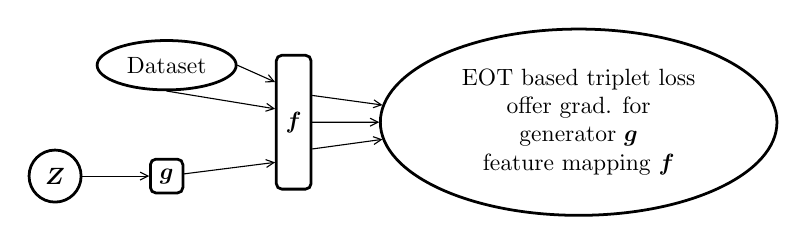
\begin{tikzpicture}
    \tikzstyle{ecnode} = [draw, ellipse, inner sep = 4pt,  align=center]
    \tikzstyle{enode} = [draw, circle, inner sep = 4pt,  align=center]
    \tikzstyle{nnode} = [rectangle, rounded corners = 2pt,draw,inner sep = 4pt]
    
    \begin{scope}[scale=0.85, every node/.append style={transform shape}]
      \node[enode] (z) at (-4,0) {$\bm{Z}$};
      % \node[enode, right=2cm of z] (x) {$\bm{X}$};
      % \node[nnode, right=2cm of x] (fx) {};
      \node[nnode, above right=-0.5cm and 3cm of z, minimum height=2cm] (f1) {$\bm{f}$};
      \node[nnode, right= of z] (g) {$\bm{g}$};
      \draw[->] (z) -- (g);
      \draw[->] (g) -- ($(f1.west) + (0,-0.6)$);


      \node[ecnode, above= of g] (dt) {Dataset};
      \draw[->] ($(dt.east) + (0, 0)$) -- ($(f1.west) + (0,0.6)$);
      \draw[->] ($(dt.south) + (0, 0)$) -- ($(f1.west) + (0,0.2)$);

      \node[ecnode, right= of f1] (gan) {\begin{tabular}{c} EOT based triplet loss \\ offer grad. for\\ generator $\bm{g}$ \\ feature mapping $\bm{f}$\end{tabular}};
      \draw[->] ($(f1.east) + (0,0.4)$) -- (gan.175) ;
      \draw[->] ($(f1.east) + (0,0)$) -- (gan.180) ;
      \draw[->] ($(f1.east) + (0,-0.4)$) -- (gan.185) ;


    \end{scope}
    % \begin{scope}[scale=1.0]
    %   \input{images/eot/triplet.tex}
    % \end{scope}
  \end{tikzpicture}
  
\end{frame}

\graphicspath{{../source/chapter8/}}

\begin{frame}[label=current]{Numerical}
  \begin{figure}[!ht]
    \captionsetup[subfigure]{justification=centering}
    \centering
    \begin{subfigure}[b]{0.44\textwidth}
      \centering
      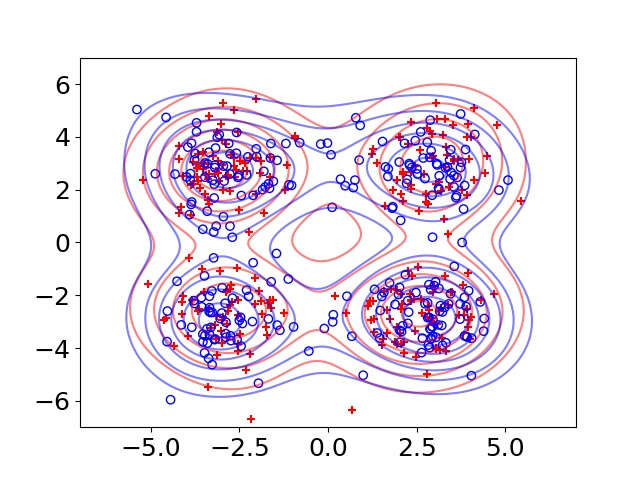
\includegraphics[width=1\linewidth]{images/toy/gauss4/frame8.jpg}\vspace{-3pt}
      \caption{}
      \label{fig-toy}
    \end{subfigure}
    % \centering
    % \begin{subfigure}[b]{0.44\textwidth}
    %   \centering
    %   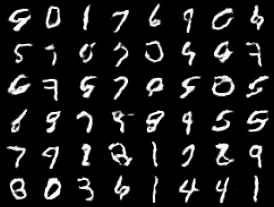
\includegraphics[width=0.8\linewidth]{images/mnist/fake/eot_18500_crop.png}\vspace{5pt}
    %   \caption{}
    %   \label{fig-fake-wgan}
    % \end{subfigure}
    \centering
    

    \begin{subfigure}[b]{0.44\textwidth}
      \centering
      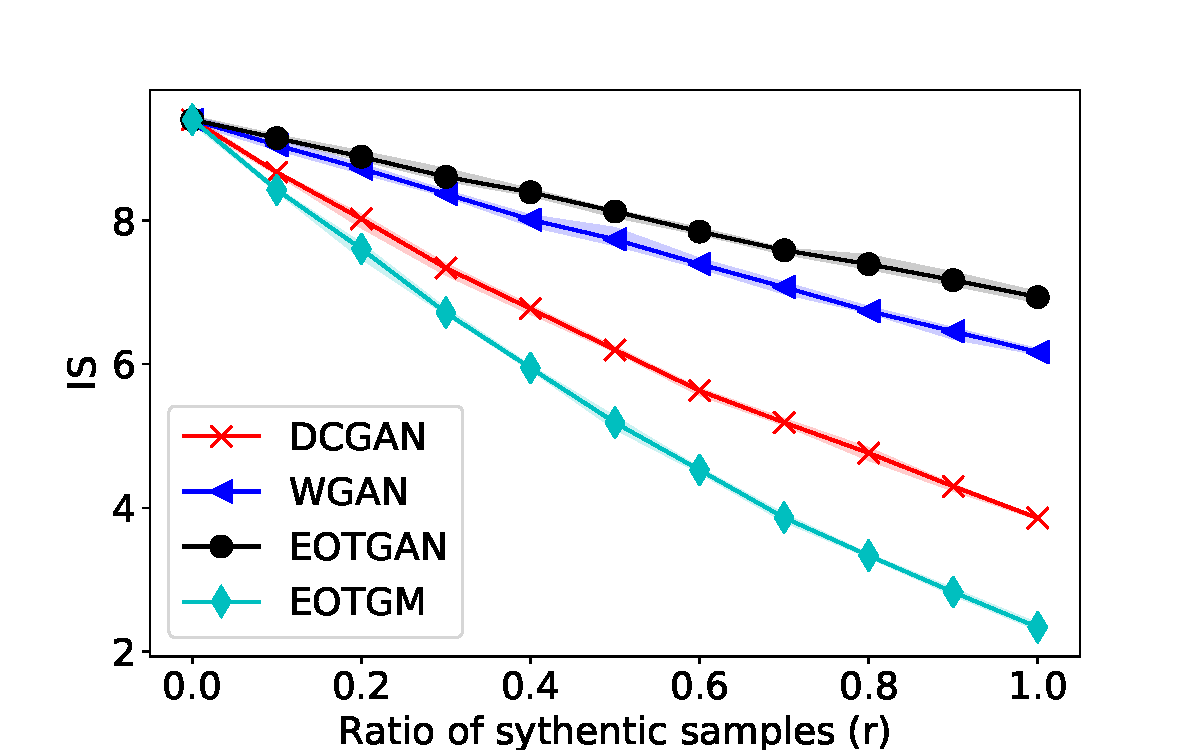
\includegraphics[width=1.1\linewidth]{images/mnist/tra_score/IS_29.pdf}\vspace{-3pt}
      % \caption{}
    \end{subfigure}
    \vspace{20pt}  
    \begin{subfigure}[b]{0.44\textwidth}
      \centering
      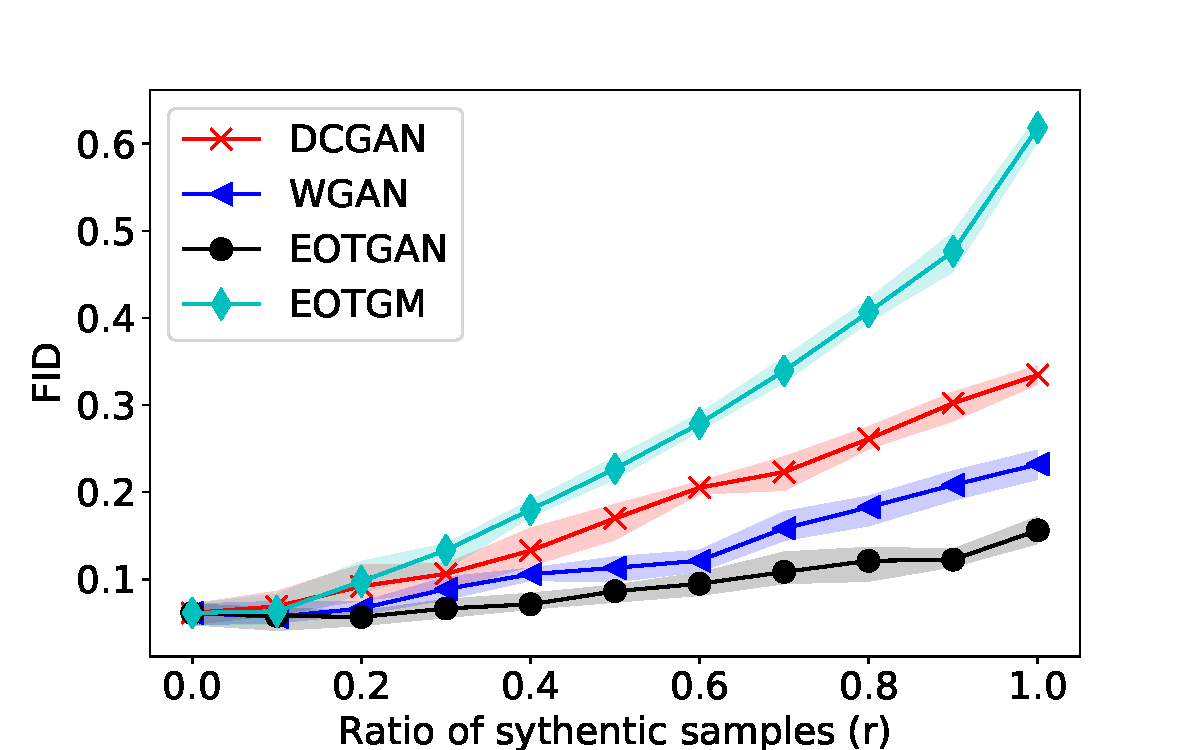
\includegraphics[width=1.1\linewidth]{images/mnist/tra_score/FID_29.pdf}\vspace{-3pt}
      % \caption{}
      
    \end{subfigure}
    % \vspace{-15pt}
    \captionsetup{labelformat=empty,justification=centering}
    \caption{Comparison of IS and FID (on MNIST) versus mixing ratio $r$. % (For
      % each model at a certain mixture ratio, $5$ experiments are
      % independently performed. Each solid curve with markers plots the mean of $5$
      % experiments with shaded areas denoting the range of corresponding
      % results.
    }\vspace{-1cm}
    
  \end{figure}

\end{frame}

%%% Local Variables:
%%% mode: latex
%%% TeX-master: "../ppgm_slide"
%%% End:



%%% Local Variables:
%%% mode: latex
%%% TeX-master: "../ppgm_slide"
%%% End:



%%%%%%%%%%%%%%%%%%%%%%%%%%%%%%%%%%%%%%%%%%%%%%%%%%%%%% 
% ------------------------------------------------
% Summary
%%%%%%%%%%%%%%%%%%%%%%%%%%%%%%%%%%%%%%%%%%%%%%%%%%%%%% 

\section{Summary and Q$\&$A}
\subsection{Summary}
\begin{frame}{Summary}
  \begin{itemize}[label=$\bullet$]
  \item Brief on probabilistic graphic models
  \item Overview of inference methods
  \item A focus on the message-passing
  \item Transition to inference methods with NN
  \end{itemize}
\end{frame}
\subsection{Q$\&$A}

{ \setbeamercolor{background canvas}{bg=hl_bg}
  \setbeamercolor{normal text}{fg=hl_fg}
  \setbeamercolor{frametitle}{fg=hl_fg}
  \begin{frame}
    \usebeamercolor[fg]{normal text}
    \begin{center}
      {\large Thank you for your attention.}\\
      {\large Q$\&$A.}
    \end{center}
    
  \end{frame}
}


%%% Local Variables:
%%% mode: latex
%%% TeX-master: "../ppgm_slide"
%%% End:





\end{document}

%%% Local Variables:
%%% mode: latex
%%% TeX-master: t
%%% End:
